\providecommand{\classoptions}{keys}
%% The next two lines are suggested at
%% to work around the following error:
%%
%%  ----------------------------
%%  /usr/local/texlive/2018/texmf-dist/tex/latex/chngcntr/chngcntr.sty:42: LaTeX Error: Command \counterwithout already defined.
%%                 Or name \end... illegal, see p.192 of the manual.
%%
%%  See the LaTeX manual or LaTeX Companion for explanation.
%%  Type  H <return>  for immediate help.
%%   ...
%%
%%   l.42 ...thout}{\@ifstar{\c@t@soutstar}{\c@t@sout}}
%%   ----------------------------
%%
%% The two lines:
\let\counterwithout\relax
\let\counterwithin\relax
%% Suggested fix above taken from
%% https://tex.stackexchange.com/questions/425600/latex-error-command-counterwithout-already-defined
%%

\documentclass[
  deliverables,
  longtasklabels,
  numericcites,
  noworkareas,
  svgnames,
  \classoptions
]{euproposal}       % for writing
%\documentclass[submit,noworkareas,deliverables]{euproposal}        % for submission
%\documentclass[submit,public,noworkareas,deliverables]{euproposal} % for public version

\usepackage[utf8]{inputenc}
\usepackage{hyperref}
% \usepackage{minitoc}
%\usepackage{varioref}

\usepackage{float}  % used to suppress floating of tables in Resources section.
\usetikzlibrary{calc,fit,positioning,shapes,arrows,snakes}
\graphicspath{{tasks/}}

\addbibresource{bibliography.bib}
% temporary fix due to http://tex.stackexchange.com/questions/311426/bibliography-error-use-of-blxbblverbaddi-doesnt-match-its-definition-ve
\makeatletter\def\blx@maxline{77}\makeatother

% %%% institutions
\WAinstitution[id=SRL,
        countryshort=NO,
        acronym=Simula]
        {Simula Research Laboratory}

\WAinstitution[id=MP,
        countryshort=DE,
        acronym=MaxPlanck]
        {Max Planck Institute}

\WAinstitution[id=QS,
        countryshort=FR,
        acronym=QuantStack]
        {QuantStack}

\WAinstitution[id=UIO,
        countryshort=NO,
        acronym=UiO]
        {University of Oslo}

\WAinstitution[
  id=XXX,
  countryshort=XX,
  acronym=XXX,
]{FIXME: Placeholder}



% \WAinstitution[id=PD,
%         countryshort=CH,
%         acronym=PersonalData]
%         {PersonalData.io}

\WAperson[id=minrk,
           personaltitle=Dr. ,
           birthdate=9 Oct. 1984,
           academictitle=Senior Research Engineer,
           affiliation=SRL,
           department=Numerical Analysis and Scientific Computing,
           privaddress=None of your business,
           privtel=that neither,
           email=benjaminrk@simula.no,
           workaddress={TODO: Simula, Oslo},
           %worktel=+33 6 77 90 32 79,
           % worktelfax=+33 6 77 90 32 79,
           %workfax=N/A
           ]
           {Benjamin Ragan-Kelley}

%%% Local Variables:
%%% mode: latex
%%% TeX-master: "proposal"
%%% End:

% LocalWords:  WAperson miko personaltitle academictitle privaddress privtel Sud
% LocalWords:  workaddress worktel workfax gc worktelfax pcg pcsa WAinstitution
% LocalWords:  shortname partof streetaddress townzip countryshort efo 3kd89
% LocalWords:  jacobs-logo.png Seefahrtstrasse Kruislann Montparnasse Universit
% LocalWords:  baz Westerfield
 % Some sections of the included files depend on this.
\usepackage{lscape} % for landscape
\usepackage{comments}
% %\usepackage[final]{comments}
\usepackage{verbatim}
\usepackage{listings}
\usepackage{supertabular,array}
\makeatletter
\newcommand\arraybslash{\let\\\@arraycr}
\makeatother
% \setlength\tabcolsep{1mm}
% \renewcommand\arraystretch{1.3}
%% Related Projects
\newcommand{\scienceproject}{\mbox{\textsc{SCIEnce}}\xspace}
\newcommand{\OOMMF}{OOMMF\xspace}
\newcommand{\OOMMFNB}{OOMMF-NB\xspace}
\newcommand{\ODK}{OpenDreamKit\xspace}
\newcommand{\VRE}{VRE\xspace}
\newcommand{\VREs}{VRE\xspace}
\newcommand{\software}[1]{{#1}\xspace}
\newcommand{\GAP}{\software{GAP}}
\newcommand{\HPCGAP}{\software{HPC-GAP}}
\newcommand{\libGAP}{\software{libGAP}}
\newcommand{\Singular}{\software{Singular}}
\newcommand{\Sage}{\software{SageMath}}
\newcommand{\SageCombinat}{\software{Sage-Combinat}}
\newcommand{\MuPADCombinat}{\software{MuPAD-Combinat}}
\newcommand{\Docutils}{\software{Docutils}}
\newcommand{\Pygments}{\software{Pygments}}
\newcommand{\Sphinx}{\software{Sphinx}}
\newcommand{\SCSCP}{\software{SCSCP}}
\newcommand{\JavaScript}{\software{JavaScript}}
\newcommand{\Python}{\software{Python}}
\newcommand{\IPython}{\software{IPython}}
\newcommand{\Jupyter}{\software{Jupyter}}
\newcommand{\JupyterHub}{\software{JupyterHub}}
\newcommand{\Cython}{\software{Cython}}
\newcommand{\Pythran}{\software{Pythran}}
\newcommand{\Numpy}{\software{Numpy}}
\newcommand{\Pari}{\software{PARI}}
\newcommand{\PariGP}{\software{PARI/GP}}
\newcommand{\libpari}{\software{libpari}}
\newcommand{\GP}{\software{GP}}
\newcommand{\GPtoC}{\software{GP2C}}
\newcommand{\Linbox}{\software{LinBox}}
\newcommand{\LMFDB}{\software{LMFDB}}
\newcommand{\OpenEdX}{\software{OpenEdX}}
\newcommand{\Linux}{\software{Linux}}
\newcommand{\LATEX}{\software{\LaTeX}}
\newcommand{\SMC}{\software{SageMathCloud}}
\newcommand{\cocalc}{\software{CoCalc}}
\newcommand{\Simulagora}{\software{Simulagora}}
\newcommand{\KANT}{\software{KANT}}
\newcommand{\Magma}{\software{Magma}}
\newcommand{\Mathematica}{\software{Mathematica}}
\newcommand{\Maple}{\software{Maple}}
\newcommand{\Matlab}{\software{Matlab}}
\newcommand{\MuPAD}{\software{MuPAD}}
\newcommand{\MPIR}{\software{MPIR}}
\newcommand{\Arxiv}{\software{arXiv}}
\newcommand{\Givaro}{\software{Givaro}}
\newcommand{\fflas}{\software{fflas}}
\newcommand{\MathHub}{\software{MathHub}}
\newcommand{\FindStat}{\software{FindStat}}
\newcommand{\GitHub}{\software{GitHub}}
\newcommand{\GitLab}{\software{GitLab}}
\newcommand{\Trac}{\software{Trac}}
\newcommand{\git}{\software{git}}
\newcommand\DKS{\ensuremath{\mathcal{DKS}}\xspace}
\newcommand{\FLINT}{\software{FLINT}}
\newcommand{\nbval}{\software{nbval}}
\newcommand{\nbdime}{\software{nbdime}}
\newcommand{\nbdiff}{\software{nbdiff}}
\newcommand{\nbmerge}{\software{nbmerge}}
\newcommand{\conda}{\software{conda}}
\newcommand{\clang}{\software{clang}}
\newcommand{\gcc}{\software{gcc}}
\newcommand{\cling}{\software{cling}}
\newcommand{\Julia}{\software{Julia}}
\newcommand{\Fortran}{\software{Fortran}}

%%% Local Variables:
%%% mode: latex
%%% TeX-master: "proposal"
%%% End:

\usepackage{framed}

\newcommand{\allparticipants}{{SRL,MP,QS,UIO,IFR}}

\newcommand{\softwarename}[1]{\texttt{#1}}
\newcommand{\repotodocker}{\softwarename{repo2docker}}
\newcommand{\binderhub}{\softwarename{BinderHub}}
% \newcommand{\mybinder}{\softwarename{mybinder.org}} % mybinder.org in monospaced font
\newcommand{\mybinder}{mybinder.org}   % mybinder.org in normal proportional font

%\newcommand*{\fullref}[1]{\ref{#1} \nameref*{#1}} % One

\newcommand*{\fullref}[1]{\hyperref[{#1}]{\ref{#1} \nameref*{#1}}}
% single clickable link of the style: 1.1 Concept
% source: https://tex.stackexchange.com/questions/121865/nameref-how-to-display-section-name-and-its-number



% longtaskref: T1.2: Title of task
\newcommand\longtaskref[2]{\csname task@#1@#2@label\endcsname: ``\csname task@#1@#2@title\endcsname''}



\begin{document}
\begin{draft}


\section*{Guidelines for proposal co-authors}

\begin{verbatim}
- Consistency. 
  - [ ] Section or section or Sect or Sec? Use 'Section'
  - [ ] Figure or figure or Fig or Fig.? Use 'Figure'
  - [ ] Binder or binder - Binder? Use 'Binder'
  - [ ] MyBinder or Mybinder or mybinder? Use `mybinder.org` for the public
        instance of the service -> \mybinder

- we have a command \repotodocker to insert 'repo2docker' in \softwarename{}
  font.
- we have a command \binderhub to insert 'BinderHub'.
- we have a command \mybinder to insert 'mybinder.org'.
- Best use {} after the commands to enforce a space, i.e. ``\repotodocker{} is the focus''

\end{verbatim}

\section*{Todo items}
- [ ] describe our relation to the Binder team

\end{draft}
\clearpage

\begin{proposal}[
  % participants
  PI=mrk,
  mrkname=Benjamin Ragan-Kelley,
  mrkaffiliation=Simula Research Laboratory,
  mrkdept=Numerical Analysis and Scientific Computing,
  mrktitle=Dr.,
  % site descriptions
  site=SRL, % Simula
  SRLacronym=Simula,
  SRLshortname=Simula Research Laboratory,
  site=MP, % Max Planck
  MPacronym=MPG,
  MPshortname=Max Planck Gesellschaft,
  site=UIO, % U Oslo
  UIOacronym=UiO,
  UIOshortname=University of Oslo,
  site=IFR, % Ifremer
  IFRacronym=Ifremer,
  IFRshortname=Ifremer,
  site=QS, % QuantStack
  QSacronym=QuantStack,
  QSshortname=QuantStack,
  % site=XXX, % template example
  % alternative: (can be combined)
  coordinator=Dr. Benjamin Ragan-Kelley,
  Cemail=benjaminrk@simula.no,
  Ctelfax=(47) XXX-XX-XXX,
  %coordinatorsite=SRL,
  acronym={SOURCE},
  acrolong={SOURCE},
  proposalnumber={SEP-210850361},
  title={Supporting Open, Useful and Reproducible Computational Environments},
  callname=Increasing the reproducibility of scientific results,
  callid=WIDERA-2022-ERA-01-41,
  % TODO: consistency with provided template
  % CALL: H2020-EINFRA-2015-1
  % TOPIC: e-Infrastructures for Virtual Research Environments (VRE)
  % Instrument: e-Infrastructures
  keywords={
  Open Science,
  reproducibility,
  reusability,
  education,
  accessibility,
  Jupyter,
  Binder,
  notebooks,
  cloud,
  EOSC,
  FAIR data,
  geosciences,
  health sciences,
  photon science
  },
  % computational mathematics,
  % GAP, Linbox, PARI, Sage, Singular, IPython, Jupyter, SageMathCloud, LMFDB, MathHub
  % Virtual research environments, MPIR, /GP
  % open source, free software, number theory, abstract algebra, notebooks
  instrument= Call: HORIZON-WIDERA-2022-ERA-01-41, %Call: H2020-EINFRA-2015-1, 3 Topic 9-2015
  challengeid = TODO,
  %challenge = {N/A},
  %objectiveid={N/A},
  %objective = TODO,
  %outcomeid = N/A,
  %outcomet = N/A,
  months=36,
  compactht]
\newcommand{\TheProject}{\pn}% \pn is defined automatically
% \input{grantagreement-history}
\ifgrantagreement
\else
\clearpage

\TODO{In this abstract we want to summarize the vision of the project;
  - Context: Open Science; what is Jupyter; Jupyter is big
  - Who are we
  - What is our goal
  - What is our strategy / concept
Points to hit:
- Open Science should be practical, not just available
- Jupyter is part of the solution
- *brief* highlight of how/why Jupyter and Binder make sense:
  - Jupyter is widely adopted
  - notebook encapsulate computation
  - Binder builds on Jupyter to enable shareable reproducible environments
  - Jupyter is web-based, enabling building services
- What we plan to do
  - improve Jupyter/Binder toward open science
  - operate Jupyter-based services on EOSC
  - Open Science training (skip?)
- Who we are
  - Core Jupyter experts
  - Domain experts motivating/validating Jupyter improvements
}


% \begin{verbatim}
% Call: Increasing the service offer of the EOSC Portal

% Title: Open Science Publication of Research Environments (OSPRE)

% Points to hit:

% - Open Science should be practical, not just available
% - Jupyter is part of the solution
% - *brief* highlight of how/why Jupyter and Binder make sense:
%   - Jupyter is widely adopted
%   - notebook encapsulate computation
%   - Binder builds on Jupyter to enable shareable reproducible environments
%   - Jupyter is web-based, enabling building services
% - What we plan to do
%   - improve Binder toward open science
%   - operate Jupyter-based services on EOSC
%   - Open Science training (skip?)
% - Who we are
%   - Core Jupyter experts
%   - Domain experts motivating/validating Jupyter improvements
% \end{verbatim}



% % (a3) prompt: Services supporting scholarly communication and open access (4M): based on existing initiatives across Europe (institutional and thematic repositories, aggregators, etc.), the services should empower researchers and research communities and initiatives with the necessary tools and functionalities for systematic publishing, analysing and re-using of scientific results beyond publications (data, software and other artefacts), as well as supporting long-term preservation and curation. The services should also enable scientific workflows with adequate metrics and monitoring mechanisms supporting career development and the monitoring of funding and research impact. Support to a catch-all repository for open research should be provided.
% 
% %  To truly achieve the societal goals of Open Science,
% %  we must make progress beyond the `mere availability' of scientific results,
% %  to the practical usability and exploitation of such data once it is made available,
% %  an area where there is much room for improvement.
% %  The Jupyter project and its ecosystem show great promise
% %  as tools for bridging this gap; for making Open Science
% %  useful and accessible to all,
% %  from researchers to educators to public citizens.
% %  The Jupyter Notebook and Jupyter ecosystem are of increasing
% %  importance in computational science, data science, academia,
% %  industry, governments, and service providers,
% %  used by millions worldwide.
% %  Jupyter notebooks have great potential to push Open Science
% %  forward because they provide a complete description of a
% %  computational study that can be turned into a publication
% %  or produce part of a publication, such as a figure,
% %  making complex tasks reproducible.
% %  The Jupyter-based Binder project adds a means to execute notebooks
% %  in specified computational environments, an aspect of reproducibility
% %  not yet widely supported.
% %  In \TheProject, we will extend the capabilities of the Jupyter
% %  tools and ecosystem to add functionality that we view as having great
% %  importance for EOSC and Open Science more
% %  widely and operate services on EOSC as a demonstration.
% %
% %  Many \TheProject partners have longstanding experience and
% %  leadership roles in the Jupyter ecosystem,
% %  and in deploying services built on Jupyter to many users across the globe.
% %  Complementary to this core expertise,
% %  we integrate partners focussing on the application of these tools from a wide range of disciplines,
% %  both to demonstrate and ensure that our developments serve
% %  real-world Open Science use cases.
% %
% 
%   To truly achieve the societal goals of Open Science, we must make progress
%   beyond the `mere availability' of scientific results as Open Access, to the
%   practical usability and exploitation of such artefacts once they are made
%   available, an area where there is much room for improvement. The Jupyter
%   ecosystem shows great promise as a collection of tools for bridging this gap;
%   for making Open Science useful and accessible to all, empowering researchers,
%   educators, and public citizens. Jupyter is of increasing importance in
%   computational science, data science, academia, industry, governments, and
%   service providers, and used by millions worldwide. Jupyter notebooks have
%   great potential to push Open Science beyond publications because they
%   encapsulate a computational study that may be part of a publication, such as
%   the creation of a figure, a major part of making complex tasks reproducible.
%   The Jupyter-based Binder project adds a means to execute notebooks in
%   specified computational environments, an aspect of reproducibility not yet
%   widely supported, and of great falue to re-using scientific results.
% 
%   Tools such as Jupyter and Binder increase the value of all existing Open
%   Access initiatives by adding the axis of interactive computability, empowering
%   researchers to produce derivative and validating (or refuting) work. Services
%   such as Binder also xpose public metrics and monitoring, supporting the
%   monitoring of research impact and career development for any users of the
%   system.
% 
%   We will (i) extend the capabilities of the Jupyter tools and ecosystem to add
%   functionality that we view as essential to and providing great value for EOSC
%   and Open Science, focused on accessibility, interactive publications, and
%   reproducibility. Based on this framework of improved Jupyter tools, it will be
%   possible to build Open Science Publication of Research Environments
%   (\TheProject), and (ii) build a range of diverse innovative open services on
%   EOSC as part of this project, both to demonstrate and ensure that our
%   developments serve real-world Open Science use cases.
% 
%   Many \TheProject partners have longstanding experience and leadership roles in
%   the Jupyter ecosystem, and in deploying services built on Jupyter to many
%   users across the globe. Complementary to this core expertise, we integrate
%   partners focusing on the application of these tools to a wide range of
%   scientific disciplines and communities, for which EOSC-hosted demonstrator
%   services are developed.

\begin{abstract}
  \TODO{Comment on Binder being a generic tool -- not limited to Jupyter}

  \TODO{Comment on Best practice guidelines and Training we deliver}
  
To increase the reproducibility of scientific results, we need find technical
solutions that enable reproducibility, and which at the same time are practical
and acceptable to the researchers who (could) use them.

The Jupyter notebook and ecosystem offers high potential for reproducibility:
(i) it is used widely, (ii) the notebook is a document that includes the
computation, and (iii) the notebook is machine executable.

Reproducibility enabled through Jupyter notebooks can have high impact due to
the wide spread use of notebooks: the notebook provides an environment for
scientific data exploration and thinking that is embraced and adopted by many.

To be able to reproduce results from notebooks, the software environment in
which the notebook should be executed needs to be created. This project is
about automating and improving ways to do this by improving and extending the
Binder project.

The Binder project automates the creation of software environments in which
notebooks can be executed, based on software specification standards that
already exist.

In this project, we will (i) investigate which fraction of existing Jupyter
notebooks are reproducible. Such reproducibility either comes from the efforts
of pioneers in the field to make their repositories 'Binder-enabled' using the
already existing Binder software. Or the reproducibility of the software environment is
provided because the authors of the notebook deposited software specifications
in a standard way with the notebook, which the binder tool correctly interprets.

We will (ii) extend the robustness of the applicability of the
Binder tools. For example, authors may not specify which version of
software they have used. Using the commit dates in the repository, an
improved Binder can attempt to identify a working version. We will
(iii) extend Binder's capabilities to broaden the applicability and
increase the positive impact on reproducibility in science. 

We will evaluate our efforts with selected and new use cases, such as
data publishing and use of Binder in HPC contexts, and invite the
community of researchers to contribute to the project. 

Many \TheProject individuals have longstanding experience and leadership roles in the
development of the Jupyter ecosystem, and in deploying services built on
Jupyter to many users across the globe. Complementary to this core expertise, we
integrate partners focusing on the application of these tools to a range of
scientific disciplines and communities.

All outcomes from this project -- including improved and new software, best
practice guides, application examples and training materials -- will be made
available as open source. 
\end{abstract}

%%% Local Variables:
%%% mode: latex
%%% TeX-master: "proposal"
%%% End:

\fi
\ifsubmit\else\setcounter{tocdepth}{4}\fi

\tableofcontents

\begin{draft}
\section*{Outline of Project (for Proposers)}

\TODO{This is the place for various READMEs not included in the final submission}

\subsection*{Vision}

An internal attempt at specifying our vision through short
(unsubstantiated) answers.

\begin{verbatim}

> 1) Who are we?

We are researchers, educators, and developers in and around the Jupyter community
at top research institutions and SMEs throughout Europe.


> 2) What is our goal?

To improve the accessibility of EOSC resources to researchers and the general public,
and improve the accessibility, interactivity, and reproducibility of computational research.


> 2.5) What is our strategy?

Our strategy has four core components:

1. Develop the Jupyter and Binder infrastructure, to improve its utility, maturity, and bring it to broader communities.
2. Operate a European Binder service, with the goal of eventually running on EOSC
3. Demonstrate that these services have value to research communities by developing specific applications in domains ranging widely from physics to life sciences to personal data management
4. Develop materials and run training to educate researchers in the ability to do reproducible computational science using the tools we develop, among others

> 3) From where do we start?

Jupyter is widely adopted in numerous communities and used by millions of researchers worldwide.
JupyterHub is a system for building hosted Jupyter services which is rapidly maturing
and being deployed at numerous universities, businesses, and research institutions.
repo2docker is a tool for automatically building reproducible computational environments using best practices for environment specifications and community standard tools such as Docker, conda, and pip.
BinderHub is software for hosting a web service built on repo2docker and JupyterHub,
where individuals can share reproducible environments for immediate and free interaction by readers in their browser.
mybinder.org is an instance of the BinderHub software,
currently serving thousands of users each day.
There are many communities not yet reached by Jupyter,
and Binder must grow beyond a single deployment.


> 4) How do we connect or differ from other projects?

...

> 5) Why are we excellent?

Jupyter has received the prestigious ACM Software System Award in 2017.
Previous winners include UNIX, TCP/IP, and the World Wide Web.

\end{verbatim}

% \subsection*{Mission statement for the grant}

% Our mission is to promote the next generation of community-developed
% open source software, databases, and services adapted to the needs of
% collaborative research in pure mathematics and applications.

% Our research will cover a wide variety of aspects, ranging from
% software development models, user interfaces \TODO{virtual
%   environments?}, deployment frameworks and novel collaborative tools,
% component architecture, design, and standardization of software
% \TODO{system?} and databases, to links to publication, data archival
% and reproducibility of experiments, development models and tools, and
% social aspects.

% It will consolidate Europe's leading position in computational
% mathematics and build on the remarkable success of the ecosystem of
% projects GAP, Python/Sage, Pari, Singular, LMFDB.

\subsection*{Description of the call}

% \verbatiminput{call_description}

% \TODO{What do we mean by ``new generation''}.

\renewcommand{\thepage}{\arabic{page}}
\setcounter{page}{1}
\black
\cleardoublepage
\end{draft}

%%% Local Variables:
%%% mode: latex
%%% TeX-master: "proposal"
%%% End:

%  LocalWords:  verbatiminput renewcommand thepage setcounter cleardoublepage


% ---------------------------------------------------------------------------
%  Section 1: Excellence
% ---------------------------------------------------------------------------

\section{Excellence}
% \subsection{Context and motivation}


\begin{draft}

In many scientific disciplines, it is common for researchers to rely on
heterogeneous computational tools and technologies to collect data, explore the
input data sets, run simulations, visualise the outcome, and share their result
with peers or with a larger audience. Often, such data analysis cycles are
iteratively refined.

For simple data sets, processes may remain manageable. However, when dealing with
larger and more complex use cases, including big data from research facilities
or High Performance Computing resources, the complexity makes iteration cycles
slower for the researchers. A complex iteration cycle also makes research
results more difficult to reproduce. Results that cannot be reproduced make
research ineffective: they create barriers towards re-using the results in
future research work, a critical aspect of open science. This situation is
exacerbated by the current and accelerating increase of the amount of scientific
data being available, including the data becoming accessible through the
EOSC-Hub. But this growing availability of data also provides a massive
opportunity for open science.

Project Jupyter has developed as one piece of various solutions to the data
deluge, by enabling the construction of computational services accessible from
anywhere, any web-browser-enabled device, with access to any data. Jupyter-based
tools such as \href{https://mybinder.org}{Binder} and repo2docker show great
promise for enabling researchers to better perform \textbf{reproducible and open
  science}. Jupyter was recognised for its contribution to data analysis in
research with the prestigious 2017 \emph{ACM Software System Award}, of which
previous winners include TCP/IP, UNIX, and the World Wide Web. It is widely used
today in research, education, and industry. We will build on these tools, both
improving their capabilities and expanding their accessibility to new
communities, both academic and demographic, in order to \textbf{further the
  mission of open science}.

In this proposal, core team members of Jupyter projects -- including
recipients of the \emph{ACM Software System Award} -- and key contributors to
the open source scientific computing ecosystem, detail improvements to the
capabilities of Project Jupyter-related tools to \textbf{facilitate reproducible science}.
By collaborating with a wide variety
of stakeholders from diverse scientific and educational domains, we aim to
demonstrate and ensure that such innovative open source tools -- built on Project
Jupyter -- are feasible, valuable, and effective in furthering reproducible and open science. The
goal is to \textbf{improve the accessibility, interactivity,
  reproducibility, and re-usability of computational research and open science.}

\end{draft}

\draftpage

%%% Local Variables:
%%% mode: latex
%%% TeX-master: "proposal"
%%% End:


\subsection{Objectives and ambition}
\TOWRITE{ALL}{Proofread 1.4 Ambition pass 2}

\subsubsection{Ambition}

\TheProject's ambition is to \textbf{improve the global reproducibility and accessibility} of scientific
tools, results, ideas, data and data analysis, and to 
\textbf{enable collaboration} among researchers and between researchers and the public.

We have these broad aims:
\begin{itemize}
\item Make it easier to perform computational research in a reproducible way
\item Educate researchers about reproducible practices
\end{itemize}

The world's computational resources are
constantly growing and science can produce ever-more interesting and useful 
data.  But \textbf{how do we enable the European and global
communities to make best use of that data?}  And \textbf{how do we enable the
public}, too?

Open science is a principle of making research
results as broadly accessible and useful as possible.  The first,
minimal step for this is making publications free to access.  The
second step for computational research is to make code and data
publicly accessible, enabling transparency and facilitating
\textbf{reproducibility} and verifiability of results.  But \textbf{merely making these
resources technically available is not the best we can do}.  There can
be many challenges with software, such as environment specifications
and resource requirements, that can be an impediment to the transition
from `technically available' to `practically useful.'  With the tools
of the open source open science community, we can do better.

\TOWRITE{}{add binder}

The Jupyter ecosystem consists of a \textbf{large, global community} of
developers and researchers producing software focused on interactive
computation and communication, and is \textbf{widely used by millions} of
individuals in numerous scientific fields, ranging from molecular
biology \cite{Wang2016} to materials science \cite{Hughes2014},
astronomy \cite{Baron2017} and climate science
\cite{Laken2015,Laken2015b}.  Jupyter software is permissively
licensed under the Berkeley Software Distribution (BSD) license,
allowing anyone to use Jupyter software for free, and even build
derivative commercial products, as has been done in the cases of
Google Colaboratory, Microsoft Azure Notebooks, IBM Watson Studio, and
others.  By contributing to the Jupyter ecosystem,
\TheProject maximises its impact, immediately benefiting the existing
large Jupyter community, and increasing the likelihood that
\TheProject's results will be maintained by the community after the
end of formal funding.

When it comes to Jupyter and Open Science for \textbf{reproducibility} we aim to improve the
\textit{status quo} by bringing the two together:

\begin{itemize}
\item Improve software in the Jupyter ecosystem to \textbf{improve reproducibility of environments}.
\item Enable researchers and the public to \textbf{better perform and benefit
  from Open and Reproducible Science}, through software, services, and education.
\end{itemize}

\TOWRITE{}{'practical reproducibility'}

Open Science that truly benefits society must be more than merely
technically accessible.  Individuals must be able to find the
resources they want and interact with them.  Ideally, they should be
able to ask new questions of models and data published by those that
came before.  This is where \TheProject fits in.  Excellent research
is being performed in all scientific fields, but making those results
practically accessible and engaging to others is a challenge.
Jupyter notebooks enable publishing code and data in a form that is
interactive, where readers can see code, run it, and see results.
They can then modify the code and produce new data and charts that the
first authors may not have considered.  Jupyter does not solve the
software installation problem, however, which can be significant for
scientific software.  For a publication to be truly interactive or
reproducible, it must include a computational environment (or a
sufficiently precise description of one such that it can be recreated)
in order to reliably be able to run for another individual.  Services
and tools such as Binder and repo2docker have started to demonstrate
that this can be facilitated: by
publishing a description of the requirements to run the software,
repo2docker is able to recreate a computational environment with
everything needed to run the software, including a Jupyter
environment for interactively exploring the resource.  Binder wraps
this in a web service, enabling immediate, free \textbf{reproduction and sharing} of
computational results on the web, with no requirements of readers
other than a web browser.
By developing these tools further, \TheProject enables researchers to
(i)~\textbf{make their results reproducible},
(ii)~allow other researchers to \textbf{reproduce or extend that research within minutes} or hours,
and (iii)~\textbf{enable the public to interact with the
science they are funding}.

By cooperating with specific applications from diverse domains in science and education,
we ensure and demonstrate that the work is valuable to a broad community of researchers, students, educators, and the public.
All together, Jupyter and Binder enable the migration of the open
science community from static publication to \textbf{truly interactive,
reproducible publications}.

The Jupyter notebook application is already TRL 8,
while the Binder software and service prototype at mybinder.org is TRL 6.
We will bring Binder to at least TRL 8 during the course of the project.


%%% Local Variables:
%%% mode: latex
%%% TeX-master: "proposal"
%%% End:

%  LocalWords:  eucommentary textsuperscript textregistered textsuperscript specialised
%  LocalWords:  textregistered recomputation textbf textbf rigourous centred flagshsip
%  LocalWords:  subsubsection realisation textit

\draftpage


\subsubsection{Objectives}\label{sect:objectives}

% \noindent The aims of \TheProject are to:

% \TOWRITE{remove aims}
% \begin{compactenum}[\myemph{Aim} 1:]
% \item Enable a
%   \myemph{sustainable}, \myemph{community-developed}, general purpose, \myemph{interoperable} toolbox for
%   interactive computing, data processing, and visualization
%   \myemph{that facilitates the entire life-cycle of open science},
%   from initial exploration to \myemph{reproducible publication}, research and development in
%   industry, teaching, and outreach.
%   This is by supporting and steering the Jupyter software ecosystem,
%   which exists to develop open source software,
%   open standards, and services for interactive computing across dozens of programming languages.
%
% \item Leverage this technology for all scientists, across borders,
%   domains, disciplines, and demographics, through
%   \myemph{free public distributed collaborative services} tightly integrated
%   into the European Open Science Cloud (EOSC),
%   in collaboration with a federation of related services
%   operated by the wider community.
%
% \item Demonstrate the value and versatility of such services through
%   \myemph{innovative co-designed tailored applications} in a variety of disciplines and
%   contexts.
%
% \item \myemph{Support open science} and maximize impact through development and
%   dissemination of best practices,
%   \myemph{training}, and \myemph{community building}
%   around the usage and development of the above toolbox,
%   with a focus on \myemph{interoperability}, \myemph{reproducibility}
%   and \myemph{reusability}.
% \end{compactenum}
% develop and support the Jupyter ecosystem in a direction that benefits and facilitates open science
%     make these tools accessible to as many people as possible via operation of free, public services
%     demonstrate and ensure that these developments are useful to real scientists and the public
%     foster open science through training of students and researchers in best practices using these tools


% \item \label{aim:facilitation}
%   Facilitate open science through the development
%   of tools enabling reproducibility, sharing, and collaboration.

% \item \label{aim:accessibility}
%   Maximise accessibility and interoperability of open science services and tools,
%   across domains, disciplines, and demographics.

% \item \label{aim:sustainability}
%   Maximise sustainability of software tools for open science
%   by developing the community and contributing
%   to and supporting community-led software efforts.



%   Support open source software for open science, and notably the
%   Jupyter ecosystem,



% \end{compactenum}

\medskip
\noindent We will achieve our ambition through the following objectives:

\TOWRITE{mention TRL goals}

\begin{compactenum}[\myemph{Objective} 1:]

\item \label{obj:reproducibility} \myemph{Facilitate reproducibility and FAIR data} ---
  improving the \myemph{reproducibility of computational environments}
  used for science, and facilitating \myemph{FAIR data practices}.
  We will contribute to the recording and reproducibility
  of environments with repo2docker and Binder,
  and extend capabilities to better support FAIR
  data requirements. In particular, the archival of execution
  environments to support \myemph{reusability} of notebooks in the future
  needs attention. Such notebooks may, for example, be published alongside
  traditional publications to detail the computation of published data
  and figures, and address the Reusability requirement of FAIR data.

\item \label{obj:broaden} broaden the impact of existing tools for reproducibility by expanding the applicable domains and use cases
\item \label{obj:demonstrators}
  \myemph{Demonstrators in science and education} ---
  We will demonstrate and ensure the versatility and value of the components and
  the services built from them,
  through applications to a number of
  domains in academic research, education, research infrastructures, SMEs, and for
  the public sector, driven through our project partners. In
  particular, we will contribute demonstrators in the following areas:
  % astronomy (\taskref{applications}{astro}), education
  % (\taskref{applications}{teaching}), fluid dynamics
  % (\taskref{applications}{application-gpu}), geosciences
  % (\taskref{applications}{geoscience}), health
  % (\taskref{applications}{opendose-analysis}), mathematics
  % (\taskref{applications}{math}),
  % and photon science (\taskref{applications}{reproducibility-xfel}),
  % involving universities, research infrastructure facilities, and SMEs.

\item \label{obj:education}
  \myemph{Outreach, engagement, and sustainability} ---
  Reach out to scientists and the wider research
  communities to encourage engagement
  and exploitation of existing tools for reproducible and open science
  for their research domains and interests.
  Educate the research communities about reproducible practices,
  and available tools for reproducible publications and policies.
  Engaging a larger community will help \myemph{ensure the sustainability} of
  the services and underlying infrastructure by distributing its
  development, hosting, and maintenance over stakeholders from a
  variety of institutions and backgrounds,
  from the private sector to public research, education
  and open government.



\end{compactenum}

\begin{table}
  \label{tab:objectives-tasks}
  \caption{
  Each objective and the tasks which further that goal.}
  \begin{tabular}{|m{.3\textwidth}|m{.7\textwidth}|}

    \hline

    \myemph{Objective} & \myemph{Tasks}
    \\\hline

    \ref{obj:reproducibility} &

    % \longtaskref{core}{maintenance}
    % \longtaskref{core}{jh-bh-conv},

    \\\hline

    \ref{obj:broaden} &

    % \longtaskref{core}{accessibility},
    % \longtaskref{core}{collaboration},
    % \longtaskref{ecosystem}{xeus-cpp},
    % \longtaskref{ecosystem}{jupyter-widgets},
    % \longtaskref{ecosystem}{teaching-tools}

    \\\hline

    \ref{obj:demonstrators} &
    % \longtaskref{applications}{astro},
    % \longtaskref{applications}{teaching},
    % \longtaskref{applications}{application-gpu},
    % \longtaskref{applications}{geoscience},
    % \longtaskref{applications}{opendose-analysis},
    % \longtaskref{applications}{math},
    % \longtaskref{applications}{reproducibility-xfel}

    \\\hline

    \ref{obj:education} &

    % \longtaskref{education}{workshops},
    % \longtaskref{education}{online-resources},
    % \longtaskref{education}{helpdesk}

    \\\hline

  \end{tabular}
  \TODO{HF: Is this table compulsory?} 
\end{table}

\draftpage
% Requirements to address here:
%
% Develop an agile, fit-for-purpose and sustainable service offering
% accessible through the EOSC hub that can satisfy the evolving needs of
% the scientific community by stimulating the design and prototyping of
% novel innovative digital services. Innovative models of collaboration
% that genuinely include incentive mechanisms for a user oriented open
% science approach should be considered.

\subsection{Relation to the Work Programme}

The \TheProject project addresses the challenges of the ``Prototyping
new innovative services'' call (ID: INFRAEOSC-02-2019).

Our strategy is based on taking the increasingly popular Jupyter
Notebook and Jupyter Ecosystem: we want to evolve and improve them
so that new innovative services based of the Jupyter tools can be developed for
the EOSC.
\medskip

There is evidence that the Jupyter Notebook is an e-infrastructure
that is useful across many domains: it is already widely adopted in
numerous communities and used by millions of researchers and educators worldwide
\cite{jupyter-grant}.

\begin{itemize}
\item \emph{Journalists} and practitioners of \emph{data-driven
    journalism} at the LA Times, BuzzFeed News, Columbia Journalism School \cite{latimes-datadesk} \cite{columbia-nytimes} \cite{data-journalism},
\item \emph{Research institutions} such as CERN, JRC, and many more,
  operating institution-wide Jupyter deployment,
\item \emph{Universities} using Jupyter as a teaching platform,
\item \emph{Large cloud providers} building commercial products on the
  top of Jupyter (Google DataLab and Colaboratory, Amazon Sagemaker, Microsoft Azure
  Notebooks),
\item \emph{Other EOSC projects}. Jupyter is already planned to become
  an important service on the European Open Science Cloud (for example
  the EOSC-04-funded PaNOSC project \cite{panosc}).
\item \emph{Data scientists}: some argue that the Jupyter Notebook is
  \emph{the} tool of choice for data scientists across domains
  \cite{Perkel2018}.
\item Over 3 million notebooks are deposited on GitHub \cite{notebookcount}.
\end{itemize}
%
\begin{figure}[tb]
  \centering\includegraphics[height=0.2\textheight]{images/jeodpp.png}
  \centering\includegraphics[height=0.2\textheight]{images/jeodpp-demo.jpg}
  \caption{\emph{Left}: The Joint Research Centre (JRC) Earth Observation
    Data and Processing Platform (JEODPP) is a heavy user of the
    Jupyter Notebook (source:
    \url{https://cidportal.jrc.ec.europa.eu/home/}), where it features
    at the top of the pyramid to help users with interactive data
    visualisation and analysis. \emph{Right}: An example
    service in which an interactive visualisation is provided through
    the Jupyter Notebook rendering of the density map of the ships
    detected from Sentinel-1 images over the Mediterranean sea during
    the period October 2014 to September 2016. \cite[Figure
    6]{Soille2018}. \label{fig:jeodpp}}
\end{figure}
%
A particular example is the Joint Research Centre Earth Observation
Data and Processing Platform (JEODPP) shown in Fig.~\ref{fig:jeodpp},
illustrating the interactive data exploration within an environment
that allows to save and communicate the data exploration
conveniently. These projects are building upon Jupyter as it is
available at the moment.
\bigskip

Within this context of a common software platform, we address the call
for prototyping innovative services:
\begin{itemize}
\item Our \TheProject proposal is focussed on developing the next generation
of the Jupyter tools to enable all domains to develop such services on
the EOSC.

\item Through the \TheProject-improved Jupyter, we will provide an
  agile and fit-for-purpose \emph{EOSC-enabled
framework} within which innovative services can be built by the
scientific communities.

\item We believe this is realistic as a multitude of (non-EOSC) services and
  use cases based on Jupyter have been developed, as sketched above.

\item We co-design the framework and the service demonstrators with
  core Jupyter developers, EGI and domain specialists from the
  scientific communities.

\item We will provide some particular services as part of the project
  (in the domains of geosciences, health,  education, and photon
  science) to stimulate the design of other novel innovative services
  to address the evolving needs of the scientific community.
\end{itemize}
\bigskip


%
% % [1] EINFRAOESC-02 call (\url{https://ec.europa.eu/info/funding-tenders/opportunities/portal/screen/opportunities/topic-details/infraeosc-02-2019;freeTextSearchKeyword=innovative;typeCodes=0,1;statusCodes=31094501,31094502;programCode=null;programDivisionCode=null;focusAreaCode=null;crossCuttingPriorityCode=null;callCode=Default;sortQuery=openingDate;orderBy=asc;onlyTenders=false)}
%
% Jupyter is an important piece of infrastructure for numerous projects funded
% by the EU and its member states, including OpenDreamKit, PaNOSC, EOSC-life,
% JEODPP \cite{Soille2018}, \TODO{citations? others?}... The \TheProject project
% will thus act like a catalyst, increasing the potential impact of all these
% projects, as well as hopefully many future projects, by strengthening a common
% software platform.
%
%
%
% % Lots of EOSC and EU-funded projects are built upon jupyter
% %
% % Opendreamkit
% % PaNOSC
% % JEODPP https://www.sciencedirect.com/science/article/pii/S0167739X1730078X?via%3Dihub
% % EOSC-Pilot
% % EGI https://ec.europa.eu/info/funding-tenders/opportunities/portal/screen/opportunities/topic-details/infraeosc-02-2019;freeTextSearchKeyword=innovative;typeCodes=0,1;statusCodes=31094501,31094502;programCode=null;programDivisionCode=null;focusAreaCode=null;crossCuttingPriorityCode=null;callCode=Default;sortQuery=openingDate;orderBy=asc;onlyTenders=false
% %
% % Jupyter is a critical piece of European e-infrastructure; this project is important for sustainability, we need not just to build upon Jupyter but to consolidate the foundations.
% %
% % We also want to enable novel use cases to enable advances in European computational and data science activities that build on the Jupyter ecosystem.
% %
% % Who is better placed than the team who built Jupyter in the first place to move Jupyter forward?
% %
% % JEODPP Image (jeodpp_new_small_4.png)
% %
% %
% % The main challenge we need to address is “Develop an agile, fit-for-purpose and sustainable service offering accessible through the EOSC hub that can satisfy the evolving needs of the scientific community by stimulating the design and prototyping of novel innovative digital services. Innovative models of collaboration that genuinely include incentive mechanisms for a user oriented open science approach should be considered.” (from Specific challenge in: https://ec.europa.eu/info/funding-tenders/opportunities/portal/screen/opportunities/topic-details/infraeosc-02-2019;freeTextSearchKeyword=innovative;typeCodes=0,1;statusCodes=31094501,31094502;programCode=null;programDivisionCode=null;focusAreaCode=null;crossCuttingPriorityCode=null;callCode=Default;sortQuery=openingDate;orderBy=asc;onlyTenders=false)
% %
% % We need to make sure to either put this phrase in and respond to how we address it, or drop the right keywords.
% %
% %
% % \TODO{We should also go through the requirements from the call [1] and
% %   show how we address those [to provide easily accessible evidence
% %   that we are addressing the call].}
% %


% ---------------------------------------------------------------------------
%  Section 1.2: Methodology
% ---------------------------------------------------------------------------
\clearpage
\TOWRITE{ALL}{Proofread 1.2 up to 1.2.10}

\TOWRITE{ALL}{Write missing sections 1.2.13 to 1.2.16}

\TOWRITE{Min/Hans}{Mention KPIs somewhere?}

\TODO{Provide contents for empty subsections at the end of section 1.}

\subsection{Methodology}\label{sec:concept_methodology}
\eucommentary{5-8 pages}





% \subsubsection{Concept}%\label{sec:concept}
%
% Open Science is the principle that science, in order to be most
% {impactful} and {socially responsible}, should be done
% {publicly}, with as much of the scientific process and products
% accessible, reviewable, reproducible and reusable by as many members of
% the global community as possible.
%
% There are exciting opportunities for Open Science for almost all academic fields
% in the modern age of computational science. As more and more research takes the
% form of code and/or data, the opportunity to share, reproduce, and reuse
% scientific work is greater than ever, even enabling new forms of
% {interdisciplinary collaboration}, and interoperable and re-usable results and
% tools.
%
%  Simultaneously, there are obstacles -- both technical and social -- to
% making open science and reproducible science a practical reality. The challenges
% include: If a researcher has code and/or data to publish, how is that best
% done? How do researchers learn {best practices for reproducible science} in
% their field? How do previously disconnected fields benefit from each other's
% work as the same computational challenges are faced again and again by different
% communities? How can scientists be encouraged to make their work reproducible?
%
% These are the questions that guide the \TheProject{} project.

\subsubsection{Supporting Open, Useful, and Reproducible Computational
  Environments}\label{sec:SOURCE}

Our project is titled ``\emph{Supporting Open, Useful, and Reproducible Computational Environments.}'':
\begin{itemize}
\item The work done is this project will be \emph{Supporting} scientists in their
  endavours to make their work more reproducible and re-usable.
\item We believe in the value of \emph{Open} science and \emph{Open} source. The
  best reproducibility and re-usability of scientific results is given through
  complete transparency of the steps taken in the derivation of a result. For
  the computational aspects this means to make all simulation and/or
  post-processing and analysis steps open source. While this may not always be
  possible, we advocate such openness as the best practice for reproducible science.

  All work done, including software, training and documentation materials, will
  be open source and available through an open access license.

  (We note that the collective development of the grant proposal you are reading
  is also done as open source, and can be inspected at
  \url{http://github.com/minrk/horizon-widera-2022} for those interested.)

\item Measures towards better reproducibility have to be \emph{Useful} and
  practical: if a proposed approach or tool burdens the scientist with
  additional work, or requires significant additional skills, it becomes less
  likely to be widely accepted.

  The philosophy we support here is that the proposed (Binder) tools for
  reproducibility are based on existing standards which are already
  adopted by many and can be considered best practice.

\item Within the wide field of reproducibility in science, we focus in this
  project on the improvement of the automatic generation of \emph{Reproducible
    Computational Environments}.
  % It is an essential step for reproducible
  % science to be able to setup the correct
  % software environment, before any attempt can be undertaken to reproduce (and
  % thus repeat) the calculation of a result obtained before.
\end{itemize}

\subsubsection{Outline of concept and methodology}

In the following we explain our concept and the technology on which this
proposed project builds in more detail.
\begin{itemize}
\item Sections \fullref{sec:reproducibility} and
  \fullref{sec:reproducibility-challenges} contextualise the proposed work
  within the wide field of reproducibility.
\item Section \fullref{sec:reproducibility-concept} summarises our concept and
  approach concisely.
\item We illustrate the reproducibility discussion with
  \fullref{sec:reproducibility-example} and provide details on some of our
  \fullref{sec:science-applications}.
\item To assist the more detailed description of the concept and the content of
  the Work Packages, we provide a \fullref{sec:terminology}
  and additional technical information in \fullref{sec:project-jupyter} and
  \fullref{seq:project-binder} in our technical appendix that forms
  Section~\ref{sec:appendix} (page~\pageref{sec:appendix}) of this document.
\end{itemize}

\noindent The methodology for this project is discussed starting in section
\fullref{sec:methodology}.


%\TODO{Do we need to keep anything from the commented out lines here?}

%
% With so much research being done that wants to be Open and Reproducible,
% how can we make Science
%
% \begin{enumerate}
%     \item as \textbf{easy} as possible to share and reproduce?
%     \item as \textbf{useful} as possible to other researchers and the public?
% \end{enumerate}
%
%
%
%
%
% \noindent Our plan for \textbf{increasing the reproducibility of scientific results} can be summarised as:
%
% \begin{enumerate}
% \item improve and maintain \textbf{common software infrastructure} used for
%   reproducing computational results,
% \item develop the Jupyter ecosystem to improve capabilities to \textbf{better
%   serve Reproducible Open Science},
% \item \textbf{guide, validate, and demonstrate} our developments through
%   collaboration with a wide variety of application domains,
% \item enable students and researchers to perform Reproducible Open Science through
%   \textbf{training and education}, and improving inclusiveness by focusing
%   these on under-served and under-represented communities
% \end{enumerate}

\medskip

\subsubsection{Reproducibility}\label{sec:concept}\label{sec:reproducibility}

Before describing the focus of the work that we propose here, we want to embed
this into the much wider context of reproducibility challenges.

We will exclude the challenges of reproducing \emph{experimental} data. Our
study starts at the point where such experimental data is available in digital
form.

We will focus on the challenge of computational reproducibility: can we carry out
the same data analysis, creation of figures and tables as they are presented in
a paper, at a later stage, and get to the same results?

Such tables and figures in a publication may be computed from the analysis of
some type of raw data which could originate an experiment, another publication,
a data base, post-processing of another data set or from executing computer
simulations.

% Where additional software, such as analysis scripts, input files
% and software for the simulation are needed,

\subsubsection{Challenges of Reproducibility}\label{sec:reproducibility-challenges}

The challenges of such ``computational reproducibility'' include:
\begin{itemize}
\item Do we know the protocol, \emph{i.e.} are the different
  processing steps for that data recorded? This could be the order in which
  analysis scripts need to be executed -- for example to compute intermediate
  results -- which will be turned into a figure in the last step?

We will call this sequence of steps the \emph{workflow}. This workflow could be
archived -- for example -- through a \softwarename{README.txt} file, or scanned
pages of a hand-written laboratory notebook as a pdf file, or as a
machine-executable script (or a Jupyter notebook).

This is particularly challenging where software is used which can only be
controlled via a Graphical User Interface, as it may require manual recording
and description of the different clicks and steps in laboratory logbook.

\item Are all the scripts and configuration files (and more generally all
software) that are needed in this process known and archived?

\item Where software is involved, have we recorded which version of that
software is needed (or was used)? If compilation is required, do we know which
compilers (and which version) and which additional dependencies are required?

\item Are there instructions how to obtain / compile the required dependencies,
and the software itself (in particular where this is about simulation-based
science or more complex analysis and interpretation software tools)?

\item Where raw data is required, is this archived, accessible, and sufficiently
documented that the format is understandable?
\end{itemize}


\subsubsection{Reproducibility concept}\label{sec:reproducibility-concept}

We can classify the reproducibility challenges listed above into different categories:

\begin{description}
\item[1. Workflow]: Are the processing commands (and their order)
correctly recorded? Do we know which part of the data set the analysis is meant
to be applied to? This is to a significant degree a question of the organisation
and documentation of the research process.

\item[2. Software environment]: Can we recreate the software environment that is
required to execute these commands?

\item[3. Importance]: Is the researcher convinced that investing effort into making
their work more reproducible is a worthwhile investment? This is a wide topic,
touching on expectations, existing cultures, lack of metrics that acknowledge
reproducibility efforts, and policies.

\item[4. Other]: There are other related topics, for example the challenge of
archival of (large) research data sets, of making the data FAIR, and the (for
some domains important) bit-wise reproducibility.
\end{description}

In this proposal, we start from practices that researchers increasingly adopt,
and which we argue are \emph{good reproducibility practices}. We propose to carry
out additional work to \emph{improve the toolset enabling this practice}.

To deal with the \emph{Workflow} challenges, we recommend to automate the
workflow steps as much as possible. In particular, the use of Jupyter Notebooks
to orchestrate the execution of commands seems effective~\cite{Beg2021}.
The use of the notebook is
perceived by many as an improvement of their research effectiveness because
it supports ``Thinking with Code and Data''~\cite{Granger2021}. A such, the
practice of using Notebooks (which helps improving research effectiveness) has
the very positive side effect of making the work more reproducible. (However, we
note that an important task of this project is to support reproducible science
that does not make use of Jupyter Notebooks.)

To deal with the \emph{Software environment} challenge, we recommend to follow
standard practices to describe software requirements. The \emph{focus of this
project is to extend the capabilities of the \repotodocker{} tool} to be able to
\emph{automatically create software environments} based on such software
requirement descriptions.

We can only partially address the \emph{Importance} challenge as this needs
concerted efforts from many stakeholders (such as employers of researchers,
research funders, publishers). However, we will offer training that advocates
the value of open science and that teaches existing best practice in
effective computational science. The step from following such best practice to
making the work reproducible is -- given the Binder tools we want to develop
further here -- relatively small, or even possible without additional effort.

The \emph{Other} challenges are mostly outside the focus of this work
(although our proposal will also assist in reproducible and FAIR data
publishing, see for example Task \taskref{applications}{data-publishing}).


% \subsubsection{Terminology and repository example}\label{sec:reproducibility-example}

\subsubsection{Reproducibility Example}
\label{sec:reproducibility-example}

\begin{figure}[htb]\centering
  \includegraphics[width=0.9\textwidth]{use-cases-binder-logbook-solution.png}
  \caption{A typical use case for Binder-based reproducibility using Jupyter notebooks in research.
            Image by Juliette Belin for the OpenDreamKit project, used under
            CC-BY-SA.}\label{fig:use-cases-binder}
\end{figure}

We start with a description of a use-case making use of existing Binder-based
tools for computational reproducibility. Start from this base-line, we can
explain what progress and additional impact we will enable through this project.

Figure~\ref{fig:use-cases-binder} depicts how a scientist can use a Jupyter
notebook and the Binder software to make her research results easily
reproducible and re-usable. In short:
\begin{itemize}
\item Scientist Jane has created a notebook that carries out computations or
  data processing and creates a figure based on those results. For the purpose
  of the introduction of this workflow, we assume that
  Figure~\ref{fig:reproducibility-example-covid} shows this figure.

\item She has made the notebook and raw data available in a public repository
  (for our example at\newline
  \mbox{\url{https://github.com/fangohr/reproducibility-repository-example}}).

\item As she has described what software is needed to execute her notebook (more
  details below), it is possible for all interested scientists (and anybody
  else, including the reviewers of this proposal) to \emph{reproduce} her
  figure:

  To reproduce the figure, one needs to visit the URL\newline
  \mbox{\url{https://mybinder.org/v2/gh/fangohr/reproducibility-repository-example/HEAD?labpath=figure1.ipynb}}
  in a browser, and then wait a minute or so for a dedicated computational
  environment to be created and started. Then select 'Run' -> 'Run all cells'
  from the menu of the interactive Jupyter notebook that will appear in the
  browser.

  At that point, the computational steps that Jane has carried out to create her
  result are repeated, and the results are \emph{reproduced}.

\item Because all the computational steps are captured in the Jupyter notebook,
  they can be inspected and interrogated if desired. In particular, the steps
  can be modified and re-executed: this allows very efficient \emph{re-use} of
  the results by other researchers.
\end{itemize}

We provide a more detailed description of the components and steps in this
process in the following sections \ref{sec:terminology} to \ref{sec:mybinder}.

The reproducibility workflow shown in Figure~\ref{fig:use-cases-binder} is
working today, and we provide estimates on the number of current users in
section \ref{sec:mybinder}. The work proposed for this project will build on
this existing technology and (i)~make it more robust and easier to use
(\WPref{reproducibility}), and (ii)~extend the functionality (\WPref{impact}) so
that the existing tools can be used in many more use cases
(\WPref{applications}).

We note in particular that the Binder-enabled workflow for reproducibility has
originally been developed to reproduce results that are created within Jupyter
Notebook (as shown in Figure~\ref{fig:use-cases-binder}). As part of this
project, we will extend the Binder tool functionality, so that reproducible
computational environments can be created and used in studies that do not make
use of Jupyter notebooks.

\begin{figure}
  \centering
  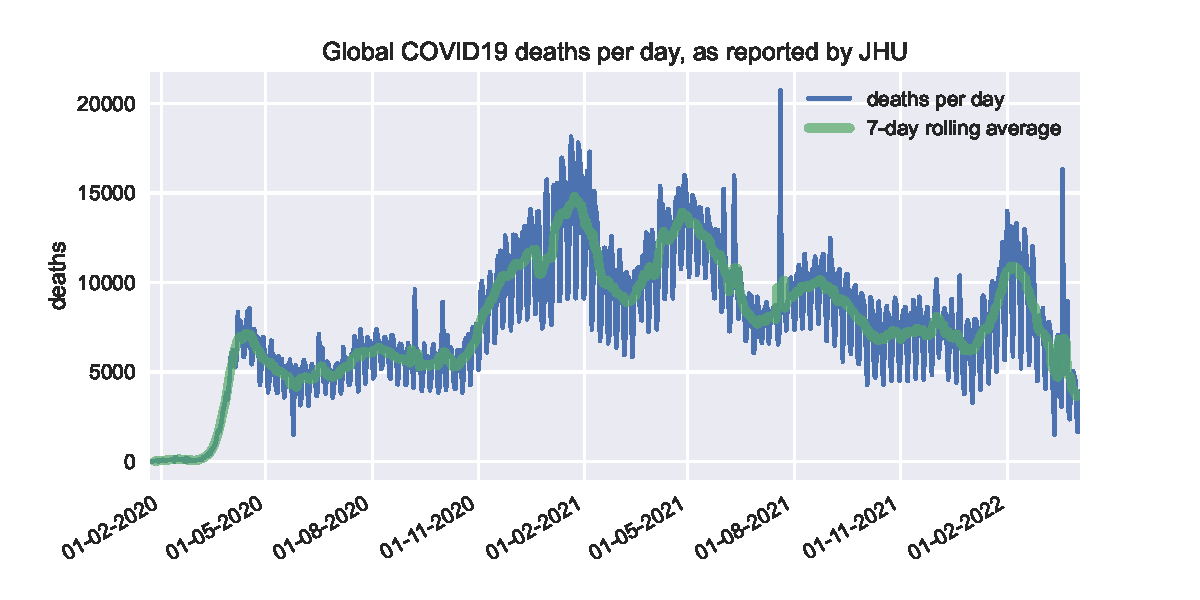
\includegraphics[width=0.8\textwidth]{images/figure1.pdf}
  \caption{Figure (\softwarename{figure1.pdf}) which can be reproduced in our explanatory repository example
    \cite{ReproducibilityRepositoryExample2022}. \label{fig:reproducibility-example-covid}}
\end{figure}

\subsubsection{Science Applications}\label{sec:science-applications}
Throughout this project, we will apply the reproducibility tools to ongoing
research projects that need reproducible processes. This is to inform the
project, evaluate the tools, and provide demonstrators. We expect the
demonstrators we develop to be exploited as production services already during
the grant, and subsequently.

Our science applications follow the workflow outlined in
\ref{fig:use-cases-binder}. \TODO{Mention that some of our science applications need
  additional features, and are not yet supported.}
\begin{itemize}
\item Introduceing reproducibility to a fish track analysis model~\cite{woillez2016} based on
  marine physics data uisng Pangeo ecosystem:
  Pangeo enables interactive analysis on HPC infrastructures~\cite{odaka2020}
  but also have examples on reproducible marine data analysis~\cite{maze2020}.
  A particular challenge here is
  the size and complexity of marine physics data to be ingested
  to obtain high spatial and temporal resolution of resulting sea bass track 
  required by fish habitat scientist.
  Access to parallel computing resources throught DASK on HPC or
  Cloud architecture together with access to bigdata stored next to the
  parallel computing architecture is required to make reproducibility realistic.
\item \TODO{Add examples from UiO}
\item Reproduciblity of result computed
  with the ab-initio software Octopus
  (\href{https://octopus-code.org}{https://octopus-code.org}) which provides a
  virtual experimentation capabilities. A particular challenge is that Octopus
  is a highly parallelised code and needs HPC computing resources for a
  reproduction of simulation results. A (Slurm) job submission may be required
  to start the reproduction.
\end{itemize}

\begin{figure}[htb]
  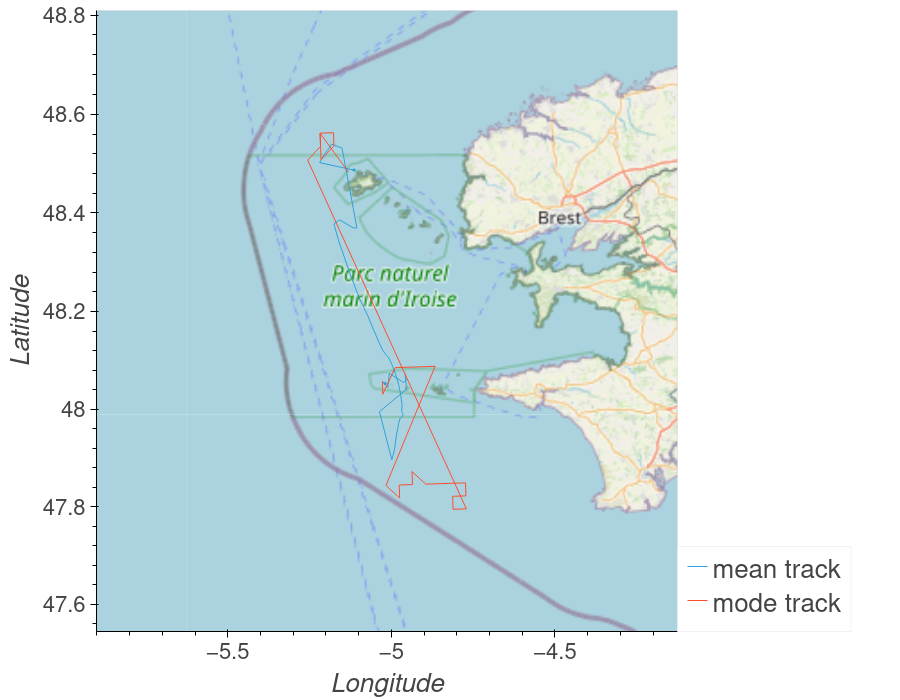
\includegraphics[width=0.33\textwidth]{images/fish.png}
  \caption{An example of an interactive analysis of  
  fish track reconstructions on a biologging tag
   data (sea bass) with low resolution marine physics data.
   % by HMM moodel ~\cite{woillez2016}} .
   (Background map: \copyright OpenStreetMap contributors ).} \label{fig:fish}
\end{figure}

\subsubsection{Methodology}\label{sec:methodology}

Our approach is centered around the following ideas:
\begin{compactenum}
  \item We put the researcher at the center of our work. In the end,
    researchers are responsible for making their work
    reproducible. It is therefore essential to find technical and social solutions
    that are \emph{useful and practical}. This idea is reflected in researchers
    being involved in \WPref{management} through the \emph{Community Engagegment
    Panel}, the requirements gathering and application of the work carried out
  in \WPref{applications} and the interaction with scientists through our
  outreach and engagement activities in \WPref{education}. All of these inputs
  drive the technical software work done in \WPref{reproducibility} and \WPref{impact}.
\item We also need to consider wishes and constraints from other reproducibility
  stakeholders. These include research councils and funders, publishers, research
  infrastructure providers, and educators. There are also opportunities to use the same
  software environment creation to support outreach and
  citizen-science projects (see~\ref{sec:mybinder}). A set of representatives of
  these domains will be gathered in the Community Engagement Panel, and connect
  us with the relevant communities. A list of confirmed panel members is
  available (see~\taskref{management}{community-engagement-panel}) and will be
  extended if the project is funded.
\item The design idea for \repotodocker{} is to build on existing standards and
  conventions. This means that researchers have already created reproducible
  repositories (if they use those conventions to specify software requirements),
  but we have not developed the tool yet to create the software for that
  repository automatically. Following this design choice means that we do not
  expect researchers to learn something just so that \repotodocker{} can
  understand it.
\item Providing useful training plays a key role in enabling and motivating
  researchers to work reproducible. We will explain the benefits for
  reproducible work, and teach good practice for reproducible science such as
  keeping raw data,  meta data and relevant software, using version control and
  automating analysis steps and workflows.
  We will also showcase tools to support the creation (and use) of reproducible
  research artifacts, including those developed through this project.
\item We will explain the possibility of using Jupyter notebooks to create
  reproducible records of computational science, but also support non-notebook
  driven use cases.
\item The measures we advocate to improve reproducibility in science are
  designed to be embedded into the ongoing research activity to minimise the
  additional burden associated with the publication of results.
\item We believe in an agile approach to effective software engineering to get
  the most useful and fast feedback from the use of those features in a real
  world context.
\item All our outputs will be open source and published with permissive
  licenses.
\end{compactenum}


\medskip
\noindent We implement our approach through 5 Work packages:

%\begin{itemize}
%\item
\WPref{management} deals with the admininstrative~(\taskref{management}{admin})
and technical~(\taskref{management}{project-management}) management of the
project, and the organisation of the Community Engagement
Panel~(\taskref{management}{community-engagement-panel}).
    % \item

    \WPref{reproducibility} will improve the robustness of reproducible
    environments through technical work on \repotodocker{} and BinderHub. In
    particular, we will first create a metric to be able to measure our progress
    (\taskref{reproducibility}{repo2docker-checker}), improve the ability create
    software environments for older repositories
    (\taskref{reproducibility}{repo2docker-timemachine}) and improve the
    performance (\taskref{reproducibility}{performance-optimisation}). We
    explicitly allocate some time in \taskref{reproducibility}{maintenance} for
    maintaining the tools we extend and want to build on. Maintenance is crucial
    to creating reliable, sustainable software, but its cost is often swept
    under the rug in funding applications because of the perceived pressure to
    focus on novelty.
    % \item

    \WPref{impact} will extend the feature set of \repotodocker{} to broaden
    the impact of the project. This
    includes to understand more data sources and software specification patters
    (\taskref{impact}{buildpacks}), to refactor the tool to not depend on a
    Kubernetis installation and support other container formats next to Docker
    (\taskref{impact}{constraints}), to export identified software dependencies,
    to support new use cases and to
    better support use outside the Jupyter ecosystem (\taskref{impact}{patterns}).
    % \item

    \WPref{applications} will test, evaluate and apply the improvements from
    work packages \WPref{reproducibility} and \WPref{impact} in real-world
    reproducibility use cases, such as best practice reproducibility show
    cases~(\taskref{applications}{demos}), use of \repotodocker{} on
    decentralised hardware~(\taskref{applications}{binder-at-home}), publishing
    of large, complex or restricted access data
    sets~(\taskref{applications}{data-publishing}), and reproducibility for HPC~
    (\taskref{applications}{binder-at-hpc}).
    % \item

    \WPref{education} disseminates outcomes, delivers training materials
    and activities, and supports community engagement. We will develop best practice guidelines for reproducible
    science (\taskref{education}{online-resources}), organise and deliver
    training events (\taskref{education}{workshops}), work closely with
    scientists wishing to contribute to the project (\taskref{education}{community-support}).
  %\end{itemize}

%
% \textbf{Improving the robustness of reproducible environments (\WPref{reproducibility})}\\
% Finally, we are explicitly allocating time in \WPref{reproducibility} for maintaining
% Jupyter software, as well as new development
%  % (\taskref{reproducibility}{maintenance}).
% Maintenance is crucial to creating reliable, sustainable software,
% but its cost is often swept under the rug in funding applications
% because of the perceived pressure to focus on novelty.
% Being up front and explicit about this cost is critical to the sustainability
% of open source open science.
%
% \medskip
% \noindent\textbf{Broadening  (\WPref{impact})}\\
% In addition to improving how successfully and how often tools like \repotodocker{} reproduce environments,
% we aim to broaden the impact of the tools by making them useful in more contexts.
% The existing software makes certain assumptions about where it will run,
% made for the purposes of limiting maintenance scope of the Binder project.
% As the project has matured, certain expansions of scope are appropriate,
% as seen in the existing demand for new features in the project.
%
% We further propose improvements to the wider Binder ecosystem
% to expand the impact of the tools in more contexts to be useful to more researchers
% and more institutions.
% In particular, we have identified planned improvements:
%
% \begin{itemize}
%   \item Binder and its crucial software component \emph{repo2docker}
%   \item relaxing Kubernetes assumption
%   \item running on HPC
%   \item more buildpacks
%     % (\taskref{ecosystem}{r2d-and-binder}).
%
% \end{itemize}
%

%   \medskip\noindent\textbf{Beyond the improvement to \TheProject tools
%   (\WPref{applications}, \WPref{education})}\\
% Beyond the improvement to the Binder tools for reproducility, we plan on
% \begin{itemize}
% \item Design, implementation, application, demonstration and
%   evaluation of multiple demonstrators, that cover research fields such as
%   \TOWRITE{}{photon and neutron science, geosciences},
%   and also interests of participating SMEs (\WPref{applications}).
% \item Producing \emph{training and education material} to disseminate
%   the ability to do reproducible computational science using the tools
%   we develop, among others (\WPref{education}).
% \end{itemize}
%
% \medskip
% \noindent
% \textbf{The science
%   demonstrators}\label{sec:science-demonstrators-in-concept}\\
%
% We describe the context and challenges for each demonstrator in this
% section. The particular planned activities are shown in the
% corresponding tasks in \WPref{applications}.


\subsubsection{Gender aspects}\label{sec:gender}

\eucommentary{Describe how the gender dimension (i.e. sex and/or gender
  analysis) is taken into account in the project's research and innovation
  content [e.g. 1 page]. If you do not consider such a gender dimension to be
  relevant in your project, please provide a justification.}

\eucommentary{
	Note: This section is mandatory except for topics which have been identified
  in the work programme as not requiring the integration of the gender dimension
  into R\&I content.
}

\eucommentary{
	Remember that that this question relates to the content of the planned
  research and innovation activities, and not to gender balance in the teams in
  charge of carrying out the project.
}

\eucommentary{
	Sex and gender analysis refers to biological characteristics and
  social/cultural factors respectively. For guidance on methods of sex/gender
  analysis and the issues to be taken into account, please refer to
  \url{https://ec.europa.eu/info/news/gendered-innovations-2-2020-nov-24\_en}
}

In order to address gender issues, \TheProject is committed to implement
communication and outreach activities for promoting the role of women and underrepresented groups in science
and STEM: i) present showcases to demonstrate the results of the project through
the eyes of female Research Software Engineers and researchers; ii)
systematically offer hybrid or online training opportunities to encompass the
lack of mobility of some potential attendees; iii) monitor gender participation
to our training, workshops, and hackathons and track progress. Members of the
consortium are involved in a number of programmes and activities who aim at
upskilling women and diversity and inclusion, for instance The Carpentries and
CodeRefinery training programmes and mentoring programs such as Outreachy or
Open Life Science.

\subsubsection{National and international research or innovation activities}

\eucommentary{Describe any national or international research and innovation
  activities whose results will feed into the project, and how that link will be
  established; [e.g. 1 pages]}
\TOWRITE{}{}

The SOURCE project, as part of the overall jupyter environment, will intrinsically build on the achievements of many national and European and international research and innovative developments, which have been produced or are being implemented in research projects in which research infrastructures and project partners are or have been involved.
Table~\ref{tab:national-research} shows a selection of highly relevant projects in different areas and coordinated and/or conducted by \TheProject partners.



\begin{table}[]
\label{tab:national-research}
\begin{tabular}{lll}
\rowcolor[HTML]{00D2CB}

Project Name  & Country & Description of the linked project and how that link will be established \\
Digital Twin  &         &                                                                         \\
Digital ocean &         &                                                                         \\
              &         &                                                                         \\
              &         &

\end{tabular}
\end{table}




\subsubsection{Interdisciplinarity}

\eucommentary{Explain how expertise and methods from different disciplines will be brought together and integrated in pursuit of your objectives. If you consider that an inter-disciplinary approach is unnecessary in the context of the proposed work, please provide a justification. [e.g. 1/2 page]
}
\TOWRITE{}{}

\subsubsection{Open science practices and implementation}

\TheProject will make use of open source licensed software, packages and libraries, following the \href{https://opensource.org/licenses}{OSI recommendations}.

All codes in this project will be Open Source and collaboratively developed using GitHub, following best software engineering practice
such as version control, tests and continuous integration.
Training materials will be collaboratively developed through the \href{https://carpentries-incubator.org/}{Carpentries Incubator}
using the \href{https://cdh.carpentries.org/}{Carpentries Curriculum Development Handbook}: all Carpentries lessons are licensed under
the \href{https://creativecommons.org/licenses/by/4.0/legalcode}{Creative Commons Attribution version 4.0 (CC-BY)} and any related software under
the \href{https://opensource.org/licenses/MIT}{MIT license}.

Use cases and showcases will only make use of data that are openly available.

All publications and/or any research data produced within \TheProject will be published Open Access.


\eucommentary{Describe how appropriate open science practices are implemented as
   an integral part of the proposed methodology. Show how the choice of practices
   and their implementation are adapted to the nature of your work, in a way that
   will increase the chances of the project delivering on its objectives [e.g. 1
   page].
%
   If you believe that none of these practices are appropriate for your
   project, please provide a justification here.
   }

\eucommentary{Open science is an approach based on open cooperative work and systematic
   sharing of knowledge and tools as early and widely as possible in the process.
   Open science practices include early and open sharing of research (for example
   through preregistration, registered reports, pre-prints, or crowd-sourcing);
   research output management; measures to ensure reproducibility of research
   outputs; providing open access to research outputs (such as publications,
   data, software, models, algorithms, and workflows); participation in open
   peer-review; and involving all relevant knowledge actors including citizens,
   civil society and end users in the co-creation of R\&I agendas and contents
   (such as citizen science).}

\eucommentary{Please note that this question does not refer to outreach actions that may be
   planned as part of communication, dissemination and exploitation activities.
These aspects should instead be described below under 'Impact'.}

\TOWRITE{}{}

\subsubsection{Research Data Management and management of other outputs}

The Data Management Plan (DMP) will be prepared and regularly updated within WP1.

Except for the usage data described below,
\TheProject activities will not generate or collect data.
While we have many demonstrators that interact with data, they do not generate or collect that
data themselves, but rather provide analytical mechanisms or access to data governed by
existing data management plans and data policies of project partners at each site,
as well as publicly accessible open data.

All data generated, collected, processed and stored will be made available following the
relevant standards and regulations. Processing of personal data in relation to training,
hackathons and/or workshop events will comply with GDPR regulations e.g. data
anonymization and minimization before sharing.
Procedures to monitor the real-time effectiveness of our dissemination and
communication strategies will also be GDPR compliant.
We have no plans to collect or produce PII during the project.

\noindent \textbf{Service usage data} \\
Any data collected through the operation of public services
(e.g. popularity data for public open science repositories)
will be fully anonymised to the satisfaction of relevant best privacy practices and regulations, such as GDPR,
and made publicly available in the standard JSON Lines format,
as is done already for mybinder.org \cite{mybinder-archive}.
This is very small data and easily archived on free hosting services such as GitHub,
and will be made available under the Creative-Commons Universal Public Domain Dedication (CC0).
There is no cost to the project associated with archiving this data long-term.


\eucommentary{
Research data management and management of other research outputs: Applicants
generating/collecting data and/or other research outputs (except for
publications) during the project must provide maximum 1 page on how the data/
research outputs will be managed in line with the FAIR principles (Findable,
Accessible, Interoperable, Reusable), addressing the following (the description
should be specific to your project): [1 page]
}

\eucommentary{
Types of data/research outputs (e.g. experimental, observational, images, text,
numerical) and their estimated size; if applicable, combination with, and
provenance of, existing data.
}

\eucommentary{
Findability of data/research outputs: Types of persistent and uniqueidentifiers
(e.g. digital object identifiers) and trusted repositories that will be used.
}

\eucommentary{
Accessibility of data/research outputs: IPR considerations and timeline for open
access (if open access not provided, explain why); provisions for access to
restricted data for verification purposes.
}

\eucommentary{
Interoperability of data/research outputs: Standards, formats and vocabularies
for data and metadata. Reusability of data/research outputs:  Licenses for data
sharing and re-use (e.g. Creative Commons, Open Data Commons); availability of
tools/software/models for data generation. }

\TOWRITE{}{}

\begin{draft}
\section*{Todo list for missing subsections}
\begin{verbatim}
- [ ] 1 page: National or international research or innovation activities
- [ ] 0.5 page: bringing together expertise and methods from different disciplines
- [ ] 0.5 page: social science and humanities - how do we integrate them, or why do we not need them
- [X] 1 page: gender dimension.
- [ ] 1 page: open science practices and implementation
- [ ] 1 page: research data management and management of other research outputs. (Also FAIR)
\end{verbatim}
\end{draft}

%%% Local Variables:
%%% mode: latex
%%% TeX-master: "proposal"
%%% End:


% ---------------------------------------------------------------------------
%  Section 2: Impact
%  ---------------------------------------------------------------------------
\clearpage
% ---------------------------------------------------------------------------
%  Section 2: Impact
% ---------------------------------------------------------------------------


\section{Impact}
\label{sec:impact}

\TODO{Review (or rewrite) section 2.2. This has not received any special attention for SOURCE
  yet.}

\subsection{Pathway toward Impact}

\eucommentary{
e.g. 4 pages
Impact: Logical steps towards the achievement of the expected impacts of the project over time, in particular beyond the duration of a project. A pathway begins with the projects' results, to their dissemination, exploitation and communication, contributing to the expected outcomes in the work programme topic, and ultimately to the wider scientific, economic and societal impacts of the work programme destination.
}

\begin{draft}
{
\textcolor{red}
%\eucommentary{
Provide a narrative explaining how the project’s results are expected to make a
difference in terms of impact, beyond the immediate scope and duration of the
project. The narrative should include the components below, tailored to your
project.

(a)	Describe the unique contribution your project results would make towards (1) the outcomes specified in this topic, and (2) the wider impacts, in the longer term, specified in the respective destinations in the work programme.
	Be specific, referring to the effects of your project, and not R\&I in general in this field.
	State the target groups that would benefit. Even if target groups are mentioned in general terms in the work programme, you should be specific here, breaking target groups into particular interest groups or segments of society relevant to this project.
	The outcomes and impacts of your project may:
  \begin{compactitem}


\item	Scientific, e.g. contributing to specific scientific advances, across and within disciplines, creating new knowledge, reinforcing scientific equipment and instruments,  computing systems (i.e. research infrastructures);
\item	Economic/technological, e.g. bringing new products, services, business processes to the market, increasing efficiency, decreasing costs, increasing profits, contributing to standards’ setting,  etc.
\item	Societal , e.g. decreasing CO2 emissions, decreasing avoidable mortality,
improving policies and decision making, raising consumer awareness.
\end{compactitem}
Only include such outcomes and impacts where your project would make a
significant and direct contribution. Avoid describing very tenuous links to
wider impacts. However, include any potential negative environmental outcome or
impact of the project including when expected results are brought at scale (such
as at commercial level). Where relevant, explain how the potential harm can be
managed.

(b)	Describe any requirements and potential barriers - arising from factors beyond the scope and duration of the project - that may determine whether the desired outcomes and impacts are achieved. These may include, for example, other R\&I work within and beyond Horizon Europe; regulatory environment; targeted markets; user behaviour. Indicate if these factors might evolve over time. Describe any mitigating measures you propose, within or beyond your project, that could be needed should your assumptions prove to be wrong, or to address identified barriers.
	Note that this does not include the critical risks inherent to the management
  of the project itself , which should be described below under
  ‘Implementation’.

(c)	 Give an indication of the scale and significance of the project’s contribution to the expected outcomes and impacts, should the project be successful.  Provide quantified estimates where possible and meaningful.
	‘Scale’ refers to how widespread the outcomes and impacts are likely to be. For example, in terms of the size of the target group, or the proportion of that group, that should benefit over time; ‘Significance’ refers to the importance, or value, of those benefits. For example, number of additional healthy life years; efficiency savings in energy supply.
	Explain your baselines, benchmarks and assumptions used for those estimates. Wherever possible, quantify your estimation of the effects that you expect from your project. Explain assumptions that you make, referring for example to any relevant studies or statistics. Where appropriate, try to use only one methodology for calculating your estimates: not different methodologies for each partner, region or country (the extrapolation should preferably be prepared by one partner).
	Your estimate must relate to this project only - the effect of other initiatives should not be taken into account.
}
\end{draft}


\TOWRITE{}{Start with brief narrative summary, hitting 'Scale and Significance' hard. We have close to nothing on Significance, yet. Scale could be clearer: All researchers!}

\subsubsection{Contributions towards outcomes and impact}
\label{sec:countributions-towards-outcome-and-impact}

The expected outputs and impact of \TheProject with respect to the
work program is detailed in Tables~\ref{table:output-comparison}
and~\ref{table:impact-comparison}, respectively.

% \begin{center}
% \begin{tabular}{|m{.3\textwidth}|m{.7\textwidth}|}\hline
%   Expected impact & \\\hline
%
%
%   Integrating co-design into research and
%   development of tools to better support scientific, industrial, and
%   societal applications benefiting from a strong user orientation &
%   The Jupyter and Binder tools have always been driven by a close connection to users; since
%   the project began as IPython in 2001, many of the developers have been
%   scientific researchers using the tools as they developed them. More recently,
%   when Jupyter has benefited from dedicated developer time, developers have
%   remained in academic institutions, in the role now referred to as
%   'research software engineers,' allowing day-to-day interactions with
%   researchers using these tools in a wide range of fields.
%
%   By supporting developers in various research institutions where the improvements
%   will be used as they are developed, \TheProject will continue this invaluable
%   collaboration.
%
%   The impact of this approach for enabling reproducible computational science is expected
%   to be very high because it is a direct response to the strong demand from
%   scientists for improving the productivity and reproducibility of their work.
%   The notebook approach central to the Jupyter community is being embraced in many scientific disciplines, so the
%   proposed services to be developed in \TheProject are strongly oriented to the user needs.
%   Further, the environment-reproducibility focus of the Binder project is useful well beyond
%   the notebook focus of the Jupyter community.
%
%   \\\hline
%
%   Supporting the objectives of Open and Reproducible Science by
%   improving access to content and resources, and facilitating interdisciplinary
%   collaborations &
%   Binder and repo2docker have seen rapid uptake in many kinds of research,
%   because they bring together the essential elements of the modern scientific
%   computational workflow (from data collection to publication and open sharing)
%   in the familiar format of a scientific notebook, with powerful functionality
%   for access to scientific content for analysis and visualisation.
%   Notebooks also embody the core concepts of open science by providing a
%   mechanism to reproduce results in publications, and collaborative
%   sharing of not just scientific results, but of the code that produced them.
%
%
%   We expect the use of notebooks in EOSC to improve access to scientific code:
%   digital documents and notebooks encourage publishing workflows, whereas code in
%   scripts or manual interactive workflows are often kept by the researchers who
%   performed them. The focus on clarity and reproducibility also helps to ensure
%   that data is meaningfully accessible, by preserving essential understanding to
%   make sense of the raw data.
%
%   We have already seen a good example of the Jupyter ecosystem facilitating an
%   interdisciplinary collaboration: the LIGO scientific collaboration shared
%   notebooks detailing the data processing steps which led to the discovery of
%   gravitational waves, using the Binder service to allow anyone to re-compute
%   the published plots. Scientists with no background in gravitational waves
%   studied these notebooks and improved the signal processing.
%   In this proposal, we want to provide this ability to a wider audience through
%   improved tools and documentation,
%   including for disciplines which rely on processing much larger volumes of
%   data \cite{ligo-open-science}.
%
%     By connecting new notebook capabilities to existing and highly used services,
%   we expect to have impacts for the users and also for the service provider.
%   The scientific users will have access to new capabilities,
%   and we anticipate adoption of new innovative ways of using the data.
%   We also expect an impact on the services themselves, in terms of usage,
%   but also in terms of capturing precious information and feedback on
%   how to evolve these services to best support open and collaborative use of
%   the data and services.
%
%   \\\hline
%
%   Facilitating Open and Reproducible Science by automating existing practices &
%   A key to our philosophy and success thus far has been automating
%   what scientists already are (or should be) doing.
%   The approaches and environment specifications used in Binder are
%   not specific to Binder, and are already widely adopted.
%   We only seek to automate this process,
%   and implement and document as many standards as we can find in use by the community.
%   By implementing what is already in use,
%   we minimise "lock-in" and meet users,
%   lowering the barrier to adoption relative to "bespoke" tools,
%   which require a large change in tooling, and significant disruption to researchers'
%   work.
%
%
%
%
%   % \\\hline
    %     \TOWRITE{ALL}{More impacts for other applications/demonstrators ...}
%
%   \\\hline
%
%
% \end{tabular}
% \end{center}

\begin{table}[h!]
  \begin{center}
    \begin{tabular}{>{\raggedright}m{.475\textwidth}m{.475\textwidth}}
      \textbf{Expected outputs from call}
      & \textbf{Expected outputs from the \TheProject project}\\\toprule
        %
        %
      Structured understanding of the underlying drivers, of concrete and effective
      interventions -- funding, community-based, technical and policy -- to increase
      reproducibility of the results of R\&I; and of their benefits;
      &
      %
        Developing a structured understanding of the technological challenges of practical
        reproducibility of software environments is a prerequisite for our work on the
        community-effort-based Binder tools (\WPref{reproducibility}, \WPref{impact},  \WPref{applications}).

        We know that the technologies such as the Jupyter Notebook and their reproducibility
        with Binder find some acceptance in the scientist community (see Section~\ref{sec:opensource})
        One of the outcomes of this project is an improved understanding of the underlying drivers
        for the wider research community to adopt or not adopt this technology as a concrete and effective action to improve the reproducibility of their results~(\WPref{education}). We expect an interplay of technical, social, community-specific and policy drivers affecting this.
        %

      \\\midrule
      Effective solutions, policy-, technical- and practice-based, to increase the
      reproducibility of R\&I results in funding programmes, in communities and in
      the dissemination of scientific results;
      &
        The Binder tools are effective and practice-based technical solutions to increase the
        reproducibility of R\&I results in funding programmes and in scientific research more widely~\cite{Beg2021}.
        The combination of Jupyter Notebooks and Binder are also effective for the delivery of
        workshops~\cite{binder-workshops} and education activities~\cite{Zeller2022} involving computation as participants can use complex
        software environments through their browser, and do not need to install any additional software locally.


      \\\midrule
      Greater collaboration, alignment of practices and joint action by stakeholders
      to increase reproducibility, including but not limited to training,
      specialised careers and guidelines for best practice.
      &
        \TheProject is developing tools that enable automatic computational reproducibility across many domains by aligning to the existing software specification practices. Having one tool that respects existing practices means it can be adopted across many domains, thus facilitating greater collaboration. We will develop best practice guidelines for reproducibility and open science, and disseminate them through training activities and materials. The staff hired for the project will be highly specialised research software engineers. We expect that voluntary contributors attracted by the project will also receive additional training for such specialised careers.
      \\\bottomrule
    \end{tabular}
  \end{center}
  \caption{Output comparison table \label{table:output-comparison}}
\end{table}


\begin{table}[h!]
  \begin{center}
    \begin{tabular}{>{\raggedright}m{.2\textwidth}m{.7\textwidth}}
      \textbf{Expected impacts from call}
      & \textbf{Expected impact from the \TheProject project}\\\toprule
        %
        %
      Increased proportion of reproducible results from publicly funded R\&I
      &
      %
        The \TheProject project will improve the ease of use tools for reproducibility,
        thereby increasing the number of reproducible research outputs.
        The project will also educate researchers to provide the motivation, required
        technical skills, and an understanding of best practice to achieve
        reproducible science outcomes.
      \\\midrule

        %
        %
      Increased re-use of scientific results by research and innovation
      &
        Reproducibility enables reusability, in particular where the reproduction
        of the results can be carried out automatically (for example using the
        tools developed and improved in the \TheProject project).

        From anecdotal evidence it is known that
        a new PhD student may need many months (sometimes exceeding 12 months) to reproduce
        a published study which is to form the basis of their new research task.
        An immediately reproducible research output made available together with the publication
        can reduce this time immensely: a binder-enabled reproducible repository may be able
        to recompute the results within an hour or a much shorter time because the process is automatic.
        % and because the PhD student (or more experience researcher embarking onto a
        % research
        % activity new to them) does not need to understand all the details of recreating the software environment and how to
        %
        % We know from PhD students we have supervised, that this initial learning phase can
        % be vastly reduced if the published result has a reproducible archive available.

        The availability of an immediately reproducible research output plays a very
        important role for modern research, where generally advances are built based on prior results.\\\midrule
        %
        %
        %
        %
      Greater quality of the scientific production.
      &
        %Reproducibility is an important concept underpinning the scientific method.
        %Re-usability of results -- often enabled through their reproducibility -- has the potential to accelerate the research significantly.

        The availability of practical reproducibility as advanced by \TheProject has the potential to
        improve the quality of scientific research through new opportunities for collaboration and interdisciplinary research:

        We have already seen a good example of the Jupyter ecosystem facilitating an
        interdisciplinary collaboration: the LIGO scientific collaboration shared
        notebooks detailing the data processing steps which led to the discovery of
        gravitational waves, using the Binder service to allow anyone to re-compute
        the published plots. Scientists with no background in gravitational waves
        studied these notebooks and improved the signal processing.
        In this proposal, we want to provide this ability to a wider audience through
        improved tools and documentation,
        including for disciplines which rely on processing much larger volumes of
        data~\cite{ligo-open-science}.\\
      \bottomrule
    \end{tabular}
  \end{center}
  \caption{Impact comparison table \label{table:impact-comparison}}
\end{table}


\subsubsection{Measuring impact}

As we are building tools for open and reproducible science, the best measure of our impact
is in the adoption and use of these tools and services based on them. This can be observed
qualitatively (anecdotal feedback and case studies) and quantitatively (counting workshop
attendees, for example).

% Much of our work will be in the form of contributions to existing
% public projects, such as Binder and Jupyter, which can be measured in our participation in
% those projects, such as code and documentation contributions, bug reports, and roadmap
% contributions.

We measure progress toward our objectives in \ref{sect:objectives}
via the following Key Performance Indicators (KPIs):
\begin{compactenum}[\textbf{KPI} 1:]
\item \label{kpi:reproducibility} Fraction of published repositories for
  which Binder tools can build the computational environment -- measuring both
  improvements in Binder tools and impact from our training efforts. We will
  implement the required methodology in
  \taskref{reproducibility}{repo2docker-checker}. (Objective 1)
    % Open publications for which the authors have made a reproducible repository available
    % through \TheProject services.
\item \label{kpi:broaden} Number of researchers who benefit from using
  \TheProject{} results in their work. Due to the open source nature of our
  outcomes, it is difficult to track this number accurately. To solicit this
  information, we can request feedback from users on forums, mailing lists and
  social media, and count the users we know directly working with
  them through \WPref{applications} and \WPref{education} for example. We expect
  to under count beneficiaries for this metric, but believe the KPI is still useful
  to measure our direct impact for better reproducibility in science. (Objective 2)
\item \label{kpi:demonstrators} Number of demonstrators enabled that make
  results from scientific research reproducible. (Objective 3)
\item \label{kpi:education} Metrics to capture the number of people that have
  made use of the training and education activities of \TheProject{}, such as
  workshop attendees, viewers of training videos, access to online documentation
  of best practice. (Objective 4)% can we track people accessing a documentation web site?
\end{compactenum}


\subsubsection{Target groups and scale of impact}

We have already discussed above that computational reproducibility affects the
majority of researchers, including those who carry out work that is not
predominantly computational.

The impact of this project will be realised through (i) the training we develop
and disseminate, and (ii) the improved Binder tools. The improved tools will
directly impact the community of researchers using Jupyter notebooks. However,
the \emph{improved functionality and applicability of the Binder tools outside Project
Jupyter} will benefit all researchers who need computational reproducibility, and
may be -- and in the long run -- more important.

\medskip

We can give some indication of the size and activity of the Jupyter notebook
community and use of the existing Binder tools: Jupyter Notebooks are used to
support research in numerous communities, including
%\begin{compactitem}
%\item
\noemph{Journalists} and practitioners of \noemph{data-driven
journalism} at the LA Times, BuzzFeed News, Columbia Journalism School
\cite{latimes-datadesk} \cite{columbia-nytimes} \cite{data-journalism};
\noemph{Data scientists} in academia, industry and services \cite{Perkel2018};
% \item
\noemph{Research institutions} such as CERN, EuXFEL, JRC, and many more,
operating institution-wide Jupyter deployment;
% \item
\noemph{Universities} using Jupyter as a teaching platform;
% \item
\noemph{Large cloud providers} building commercial products on the
top of Jupyter (Google DataLab and Colaboratory, AWS Sagemaker, OVH AI Notebook);
% \item
within the \noemph{European Open Science Cloud}, Jupyter is used in many EOSC
projects, and a JupyterHub service is provided by the EGI foundation.
% \item
This impact was recognised by the \emph{ACM Software System Award} that was
awarded to the Jupyter team to honour \emph{"developing a software system that
had a lasting influence"} in 2017. (Prior recipients include \emph{Unix},
\emph{TCP/IP}, and the \emph{World Wide Web} \cite{acm-award}.)

There are at least 8 million notebooks deposited on GitHub \cite{notebookcount}, and
the size of the Notebook user base was estimated to be of the order of
millions in 2015 \cite{jupyter-grant}. We know that the public Binder-based service mybinder.org
was used to create over 10,000,000 computational environments
from at least 50,000 unique repositories in 2021~(Section~\ref{sec:opensource}).

\TODO{Or integrate into table above?}
\TODO{This is mentioned on the evaluation form for this section, and then
  section is short. We should write something here.}


\subsubsection{Potential barriers}

While a number of the partners have worked closely together in previous
projects, the integration of new partners from different disciplines will
require some efforts for communication within the project.

A central barrier towards impact would be if the research community would not
accept or embrace the tools and practical best guidance developed here. To
minimise this risk, we'll stay in close touch with all our stakeholders
(\WPref{management}, \WPref{applications}, \WPref{education}), and use
the experience of the team members who are research active themselves.

A detailed assessment of risks and mitigations can be found in \ref{sec:risks}.

\subsection{Measures to maximise impact - Dissemination, exploitation and communication}

\eucommentary{
e.g. 5 pages, including 2.3
}

\begin{draft}
  \textcolor{red}
Describe the planned measures to maximise the impact of your project by providing a first version of your ‘plan for the dissemination and exploitation including communication activities’. Describe the dissemination, exploitation and communication measures that are planned, and the target group(s) addressed (e.g. scientific community, end users, financial actors, public at large).

Please remember that this plan is an admissibility condition, unless the work programme topic explicitly states otherwise. In case your proposal is selected for funding, a more detailed ‘plan for dissemination and exploitation including communication activities’ will need to be provided as a mandatory project deliverable within 6 months after signature date. This plan shall be periodically updated in alignment with the project’s progress.

Communication measures should promote the project throughout the full lifespan of the project. The aim is to inform and reach out to society and show the activities performed, and the use and the benefits the project will have for citizens. Activities must be strategically planned, with clear objectives, start at the outset and continue through the lifetime of the project. The description of the communication activities needs to state the main messages as well as the tools and channels that will be used to reach out to each of the chosen target groups.

All measures should be proportionate to the scale of the project, and should contain concrete actions to be implemented both during and after the end of the project, e.g. standardisation activities. Your plan should give due consideration to the possible follow-up of your project, once it is finished. In the justification, explain why each measure chosen is best suited to reach the target group addressed. Where relevant, and for innovation actions, in particular, describe the measures for a plausible path to commercialise the innovations.

If exploitation is expected primarily in non-associated third countries, justify by explaining how that exploitation is still in the Union’s interest.

Describe possible feedback to policy measures generated by the project that will
contribute to designing, monitoring, reviewing and rectifying (if necessary)
existing policy and programmatic measures or shaping and supporting the
implementation of new policy initiatives and decisions.
\begin{compactitem}
\item	Outline your strategy for the management of intellectual property, foreseen protection measures, such as patents, design rights, copyright, trade secrets, etc., and how these would be used to support exploitation.
	If your project is selected, you will need an appropriate consortium agreement
  to manage (amongst other things) the ownership and access to key knowledge
  (IPR, research data etc.). Where relevant, these will allow you, collectively
  and individually, to pursue market opportunities arising from the project.
\item If your project is selected, you must indicate the owner(s) of the results (results ownership list) in the final periodic report.
\end{compactitem}
\end{draft}


\TheProject is contributing to tools for Open and Reproducible Science.
Tools only have impact when they are used,
so it is important that we disseminate our work
in order to reach and support user communities so that they may best exploit our software and services. This section
outlines how the project will establish and organise the dissemination, communication, and exploitation
actions to promote the project and the adoption of its outcomes beyond the project's lifetime.


% The dissemination and communication plan is outlined in the following sub-sections.
% Therein we distinguish:
% \begin{itemize}
% \item Dissemination as the public disclosure of the results of the project through
% a process of promotion and awareness-raising right from the beginning of a project.
% It makes research results known to various stakeholder groups (like research peers, industry
% and other commercial actors, professional organisations, policymakers) in a targeted
% way, to enable them to use the results in their own work.
% \item Communication as the strategic and targeted measures for promoting the project
% and its results to a multitude of audiences, including the media and the public, and possibly
% engaging in a two-way exchange. The aim is to reach out to society as a whole and
% in particular to some specific audiences while demonstrating how EU funding contributes to tackling
% societal challenges.
% \end{itemize}

\subsubsection{Dissemination of results}

 \TheProject endeavours to make Open and Reproducible Science practices both more understandable and actionable
 to practitioners through the development and use of open and freely available tools.
Most of \TheProject software will be in the form of contributions to existing projects,
which will be governed by the licenses of those projects.
All Jupyter and Binder software is released under the permissive BSD license,
which specifically allows commercial exploitation,
as has proven successful in enabling collaborations with industrial partners
such as Google, Microsoft, IBM, and more.
Any other developments will  be made publicly and freely available under Open Source licenses, and
hosted on public code hosting sites such as GitHub.
This means that all \TheProject software will be available and accessible to all who find it,
at no cost to \TheProject,
enabling long-term access beyond the funding of \TheProject.
Similarly, non-code products such as dissemination works
(workshop materials, etc.) will be made freely available under open Creative Commons licenses.


All the partners will be involved in the dissemination of \TheProject results (see draft plan of the
dissemination, communication and exploitation plan in the text box below) and
\WPref{applications} and \WPref{education} will play a central role.

As a result, the primary dissemination effort is to:

\begin{enumerate}
  \item make sure that prospective users are \textbf{aware of the work} through \textbf{show cases, science demonstrators, demos}, and
  \item enable them to use the tools through \textbf{learning resources, training, and services}.
\end{enumerate}

Our focus for dissemination will be on
\taskref{education}{workshops}
operating workshops, training various communities in the availability,
purpose, development, and use of \TheProject software and services.
We will make a particular effort to use these workshops as an opportunity
to \textbf{support diversity and inclusion in the Open Science community},
by running (online, hybrid or in-person) workshops for under-served and under-represented groups in the academic and
open source communities. \textbf{Free and online training} will be streamed (Twitch),
 make available to the wider community for instance on YouTube and archived on Zenodo for long-term availability and
 findability to the wider community who may not be able to attend workshops.


These resources will be hosted on free, public hosting services,
such as GitHub Pages, YouTube channels and as much as possible co-developed and co-hosted with existing and
well-established organizations
(The Carpentries\footnote{https://carpentries.org/}, CodeRefinery\footnote{https://coderefinery.org/}, 
Galaxy Training Network\footnote{https://training.galaxyproject.org/}, Pangeo\footnote{http://gallery.pangeo.io/}, etc.).

We will also disseminate our results through publications and conferences.
All publications funded by \TheProject will be \textbf{Open Access},
and sites expecting publications have budgeted funds for paying Open Access fees.
We will identify and attend appropriate conferences for disseminating our work,
including running tutorials at conferences in historically interested communities such as PyData and SciPy.
Also, we will identify and attend conferences from complementary communities such as ROpenSci,
Mozilla Science, and Julia
as well as domain specific conferences to maximise the impact of \TheProject and to broaden its
audience outside the
traditionally included communities.

The operation of prototype services in \WPref{applications} is also a dissemination activity,
as services like Binder not only enable Open and Reproducible Science by facilitating interactive publications,
they also enable \textbf{interactive demonstration of tools and functionality}
developed in \TheProject.

\TheProject will also actively seek for collaboration (through the Community
Engagement Panel and
\TheProject partners) with existing EOSC projects (many already use/deploy
Jupyter Notebook services) to inform and support them in exploiting \TheProject
developments and adapting their service offerings.
\subsubsection{Exploitation}

Our primary outputs are in the form of software tools, prototype services, and information resources,
all of which will be freely available to all under appropriate permissive open licenses.
This means that exploitation generally has the form of:

\begin{compactenum}
  \item Use of Binder tools for producing reproducible environments in research, as enabled by \WPref{reproducibility}
  \item Use of Binder tools for evaluating reproducible environments in research or publication policy, as enabled by \WPref{reproducibility}
  \item Use of Binder tools in the construction and operation of services, as enabled by \WPref{impact}
  \item Deploying new services derived from our science demonstrators in \WPref{applications}
  \item Application of effective practices for reproducibility, developed and disseminated in \WPref{education}
  \item Commercial exploitation via product development and consulting \TOWRITE{Sylvain}{brief bullet here, more below}
\end{compactenum}

A key aspect of our exploitation strategy is to focus our work on existing,
active projects in Binder and the wider Jupyter ecosystem.
This means that our contributions are of immediate practical benefit to between
thousands and millions of users worldwide \TOWRITE{}{Pull in Jupyter usage info here, now that Jupyter section is gone?}.

\TheProject contributions to Binder tools will be immediately (\emph{i.e.
  already during the duration of the project}) exploited via the public mybinder.org service
and its thousands of daily users (Section~\ref{sec:mybinder}), as well as many BinderHub instances worldwide.

The science demonstrators in \WPref{applications} are themselves exploitations of the outputs
in \WPref{reproducibility} and \WPref{impact},
building services not possible before the project.
Continued operation and adoption of these services by project partners and the researchers they serve beyond 
the duration of the project is already ensured for a majority of the science applications and will indicate 
successful exploitation of the project.

%\TOWRITE{ALL}{Specific per-site exploitation?}  Not needed I think - we have
%the demonstrators clearly mentioned.

The QuantStack SME provides commercial support and development services around the
open-source scientific computing ecosystem. The team has specialized on the Jupyter ecosystem
and package management solutions, which are both at the core of this proposal. The consolidation
of Binder's technical foundations will help QuantStack provide robust solutions to its clients.

Industrial use cases met by QuantStack also show that the reproducibility issues addressed in this proposal go
beyond the scientific use case:

\begin{compactitem}
\item For example, financial institutions using numerical libraries to price and hedge derivatives must be able
   to reproduce results obtained with past versions of their software, especially in cases of mispricing or
   mishedging. Rolling back to a state of the software environment as of several years earlier may prove
   extremely difficult. Adopting the approach of Binder to favor reproducibility has shown to be a viable way
   to address this issue.
\item Similarly, in the field of industrial robotics, QuantStack has developed a conda-based distribution of the
   ROS open-source ecosystem called RoboStack, and a tool akin to repo2docker to produce container images providing
   all required packages for a ROS node, that will directly benefit from this work.
\end {compactitem}

This shows that techniques that arose from the scientific computing and research communities to address reproducibility
will help address the same issue for a much broader audience.

\subsubsection{Communication activities}

The main goal of the communication activities is making sure that potential users
are aware of the tools and services developed by \TheProject
on an ongoing basis,
showing the public clear benefits of the work they have funded.

In order to maximise this impact, it is vital to address the audience as one project
and ensure the immediate recognition of information stemming from it.
Together with all partners involved, \TheProject will therefore build \textbf{a strong project identity}
(see draft of the communication, dissemination, and exploitation plan above) to strengthen the project
identity and to deliver clear messages to our audience.

As indicated in our draft communication, dissemination, and exploitation plan, we will operate a \textbf{website}
(\taskref{management}{website}) for collecting and sharing information about \TheProject and its progress.
It will provide a centralised way to access the various publicly available deliverables, publications
and articles related to the project. The site will be regularly updated over the lifetime of the project
with the project publications and public materials, such as flyers, posters and
public deliverables, organised workshops, available services, news, etc.
Site analytics will be associated with the project website, in order
to provide useful insight on how to improve its impact. In addition, the project intends to
develop its presence on \textbf{the social and content
networks}, such as Twitter. The channels will be used for interaction
with the professional community as well as the general public
(differentiation on the content per channel based on the target group wishing to address).
As part of the project's communication plan, \TheProject will develop a social media strategy
in order to increase outreach and social impact, which can be summarised as follows: (a) identifying target
audience and key stakeholders, (b) updating social media content and sparking
discussion in social media/tweeting, (c) measuring social impact and reassessing
social media strategy as required.

\subsubsection{Communication, Dissemination, and Exploitation plan}

We will continually refine our Communication, Dissemination, and Exploitation plans, starting with the draft below:

\begin{framed}

  \centerline{\textbf{ \TheProject DRAFT COMMUNICATION, DISSEMINATION, and EXPLOITATION}}
  {
  \begin{itemize}

\item Logo creation, standard document templates for deliverables, reports, letters, presentations, roject posters/leaflets, etc. and creation and/or use of relevant social media accounts such as Linkedin, Twitter, YouTube channel (80k Twitter followers for @ProjectJupyter, 34k for @IPythonDev, and 132k for the PyData Youtube channel);
\item Annual plan for publication in scientific and technical peer-reviewed journals and conference proceedings;
\item Creation of \TheProject website:
\begin{itemize}
\item links to \TheProject repository of results (videos, training material, use cases, demonstrators, software and associated documentation such as repo2docker, JupyterJub and Binder);
\item links to social media accounts, e.g. on Facebook, Instagram, LinkedIn and Twitter and public communication channel (Zulip);
\item live “Infoboard” to highlight news and outcomes, event calendar, public resources, specific social media posts; This infoBoard will be relayed by the News (and Newsletter) of partnered projects (Jupyter, Pangeo, Ifremer, NeIC, Sigma2, etc.).
\item links to the EOSC catalogues of services and national/institutional services supporting \TheProject;
\end{itemize}
\item Use the Community Engagement Panel to review the target audience for dissemination (workshops, training, hackathon, etc.), create a live list of communication partners and associated channels and tools;
\item Coordinate (annually) with other initiatives (The Carpentries, codeRefinery, Jupyter, Pangeo) for the collaborative development of training material and the delivery of demos, training/workshops/hackathons;
\item Refine measurable goals (based on inputs/feedback from the Community
  Engagement Panel), quantitative KPIs for dissemination and monitoring procedures;
\item Develop and maintain a live collaboration plan for links and interactions with other projects (EC-funded, Nordic and/or national projects), research institutions and industries to find opportunities to show-case \TheProject results.
\item Develop a consolidated exploitation to ensure the long term and sustainable exploitation of the project results beyond its lifetime, in particular the deployment of EOSC services.
    \end{itemize}
}
\end{framed}

\clearpage
\subsection{Summary}

\eucommentary{
Provide a summary of this section by presenting in the canvas below the
key elements of your project impact pathway and of the measures to
maximise its impact.
KEY ELEMENT OF THE IMPACT SECTION
}

% measured original color as 0, 0.75, 0.95
% but it's a bit low-contrast

\definecolor{summaryblue}{rgb}{0, 0.7, 0.9}
\newtcolorbox{summarybox}[1]{
    colback=white,
    colframe=summaryblue,
    fonttitle=\bfseries,
    title={#1}
}

\begin{multicols}{2}

\begin{summarybox}{SPECIFIC NEEDS}
\eucommentary{What are the specific needs that triggered this project?}

Reproducibility is a widely recognized challenge in computational science.
There are many tools that solve \emph{part} of the problem,
or aim to solve the whole problem while requiring wholesale adoption of a specific tool,
which may not be practical or desirable across a variety of domains or communities.
Reliably reproducing software environments without requiring adoption of any single toolchain
allows for modular adoption, integrating into policies, practices, etc.
We want to lower the practical barrier to reproducibility, and thereby increase the adoption of reproducible practices.
\end{summarybox}

\begin{summarybox}{D \& E \& C MEASURES}
\eucommentary{What dissemination, exploitation and communication measures will you apply to the results?}

\textbf{Exploitation:} All services based on BinderHub will immediately benefit from the project, improving tools
already used by hundreds of thousands of users. They will also enable the application of public policies that advocate
or require reproducibility of scientific outputs. Beyond Binder, underlying software components such as repo2docker
are used in other parts of the ecosystem to enable the customization of software environments. This is the case in the
PlasmaBio project, a Jupyter-based platform at Université de Paris for education in genomics. Such projects will also
directly benefit from the improvements to repo2docker.

The QuantStack SME will exploit the improvements to Binder and it's technological foundations, in areas ranging from
industrial robotics to quantitative finance.

\textbf{Dissemination:} Results, insights, tools, and guidelines will
  be disseminated to potential users and stakeholders through conventional
  academic channels, in-person and remote workshops, websites, video tutorials
  and social media.

\textbf{Communication:} The media and general public will be informed
  about the project through news releases, videos, a website, social media,
  further media engagement, fliers and interviews, with a consistent visual
  identity.
\end{summarybox}

\begin{summarybox}{EXPECTED RESULTS}
\eucommentary{What do you expect to generate by the end of the project? }

\textbf{Improved software tools for reproducing computational environments}:
by improving the Binder tools for reproducible environments,
it will be easier for researchers to produce and share results openly and reproducibly.

\textbf{Improved understanding of good practices for reproducibility}: study results, documentation, and workshops will aid researchers and policy makers in understanding the most appropriate practices to adopt in their pursuit of reproducible research.

\end{summarybox}

\begin{summarybox}{TARGET GROUPS}
\eucommentary{Who will use or further up-take the results of the project? Who will benefit from the results of the project?}

\textbf{Computational science practitioners}: researchers with an interest in reproducibility of their on work.

\textbf{Research institutions}: institutions facilitating or enforcing the reproducibility of their researchers.

\textbf{Policy makers}: Funders and institutions requiring their subjects to follow reproducible practices

\textbf{Publishers}: Requiring/enabling reproducible publications
\end{summarybox}

\begin{summarybox}{OUTCOMES}
\eucommentary{What change do you expect to see after successful dissemination and exploitation of project results to the target group(s)?}

\textbf{Adoption of Binder tools for reproducibility}:
practitioners will have access to Binder tools for reproducibility.
Having improved their usability and robustness

\textbf{Facilitating practical policies for reproducible publications}
\end{summarybox}
\begin{summarybox}{IMPACTS}
\eucommentary{
What are the expected wider scientific, economic and societal effects of the project contributing to the expected impacts outlined in the respective destination in the work programme?
}

\textbf{Improved reproducibility of scientific results}: Improving the \emph{ease of use} tools for reproducibility
lowers the barrier for adoption, and thereby increases the number, quality, and
access of reproducible research outputs.

\textbf{Increased re-use of scientific results}: Practical reproducibility
enables rapid re-use of published results leading to more effective research activities.
\end{summarybox}
\end{multicols}
\clearpage

% \noindent
% \fbox{
% \begin{minipage}{
% % \dimexpr\linewidth-2\fboxrule-2\fboxsep
% 2in
% }
% \textbf{SPECIFIC NEEDS 2}
%
% xyz
% \begin{compactenum}
% \item x
% \item y
% \end{compactenum}
% \end{minipage}
% }
% {
% \hfill\makebox[0pt]{\fbox{
% \textbf{SPECIFIC NEEDS}}}
% \hfill
% }

% \textbf{SPECIFIC NEEDS}
%
% xyz
% \begin{compactenum}
% \item x
% \item y
% \end{compactenum}




%%% Local Variables:
%%% mode: latex
%%% TeX-master: "proposal"
%%% End:


\clearpage

% ---------------------------------------------------------------------------
%  Section 3: Implementation
% ---------------------------------------------------------------------------

\section{Quality and efficiency of the implementation}
\COMMENT{Typical granularity: 5-8 work packages with 3-5 tasks and one
  deliverable per task; 10 milestones}

\subsection{Work Plan and resources}

\label{sect:workplan}

\eucommentary{Please provide the following:\\
\begin{compactitem}
\item
brief presentation of the overall structure of the work plan;
\item
timing of the different work packages and their components (Gantt chart or similar);
\item
detailed work description, i.e.:
\begin{compactitem}
\item
a description of each work package (table 3.1a);
\item
a list of work packages (table 3.1b);
\item
a list of major deliverables (table 3.1c);
\end{compactitem}
\item
graphical presentation of the components showing how they inter-relate (Pert chart or similar).
\end{compactitem}
}

\subsubsection{Quality and efficiency of the implementation}\label{sec:workplan-structure}

\ifgrantagreement The \else As shown in Table~\ref{fig:wplist} and
Figure~\ref{fig:workpackages}, the \fi work plan is broken down into five work
packages: \WPref{reproducibility} focuses on robustness improvements of the
Binder tools, \WPref{impact} is advancing the Binder tools feature set to
increase the impact of the tools and project, \WPref{applications} applies and
evaluates the reproducibility tools in real-world research contexts.
\WPref{education} is focused on engaging with and educating researchers and the
wider public in best practices for reproducible science. This is complemented by
the usual management work package (\WPref{management}).

The Gantt chart in Figure~\ref{fig:gantt} on page~\pageref{fig:gantt} illustrates the timeline for the various tasks for
these work packages. 
%, including inter-task dependencies.

\ifgrantagreement\else
%\makeatletter\wp@total@RM{management}\makeatother
\wpfigstyle{\footnotesize\def\tabcolsep{3.5pt}}
%\wpfig[pages,type,start,end]
{\wpfig}
\fi

\begin{figure}[htb]
  \centering
  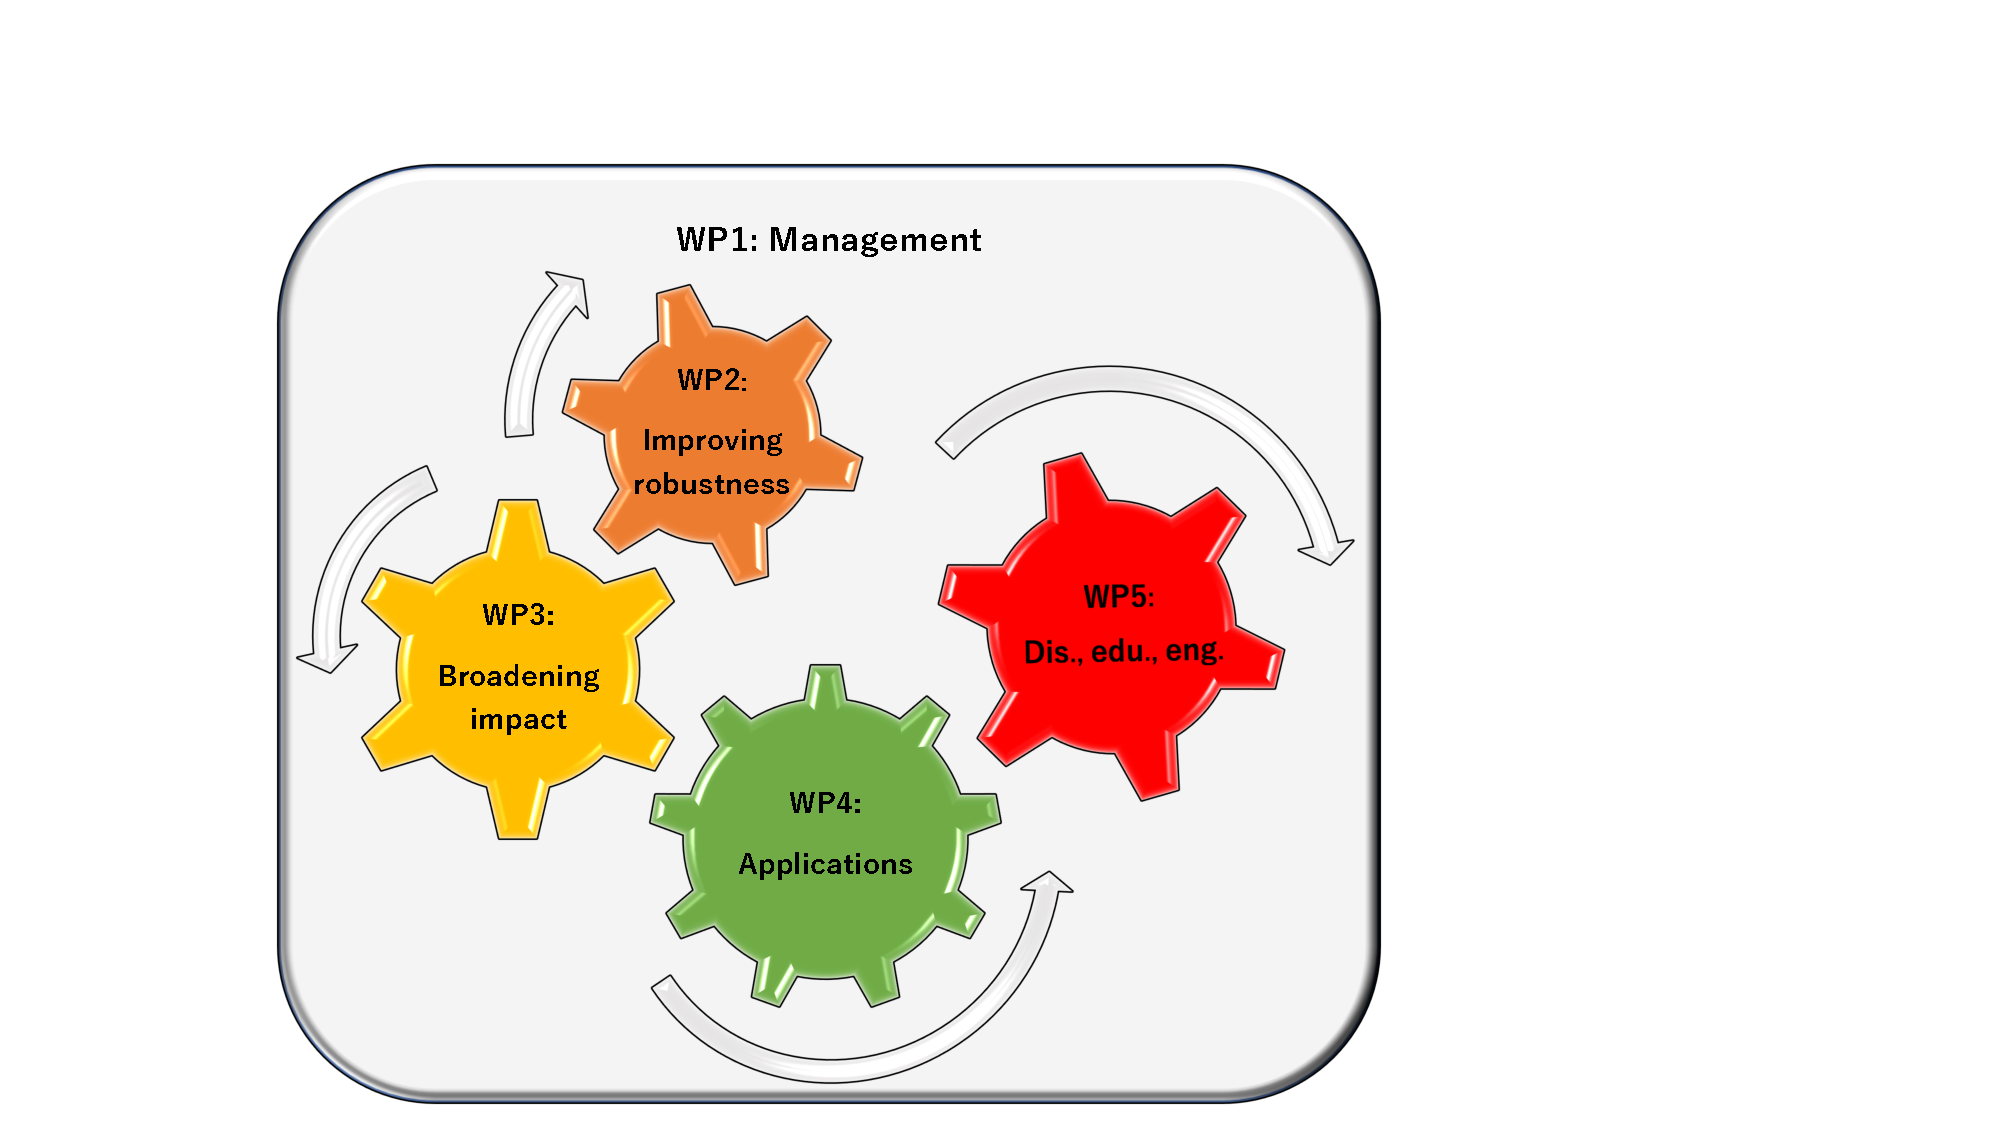
\includegraphics[width=0.7\textwidth]{images/WP.pdf}
  \caption{
    \label{fig:workpackages}
    The relationships and interactions of the work packages,
    broken up into four categories: Management (WP1),
    Development of new functionality surrounding Jupyter's Binder tools to improving robustness 
    and Broadening impact (WP2, WP3),
    Applications of tools developed in real world research context (WP4),
    and Dissemination, education, and engagement (WP5: Dis., edu., eng.).
  }
\end{figure}

% \subsubsection{How the Work Packages will Achieve the Project Objectives}
% \label{sssec:how_the_work_packages_will_achieve}

\ganttchart[draft,xscale=.4,milestones,yscale=0.9,step=3]

\TODO{HF: Don't know how to add extra text to (or override) caption to gantt chart
  (\ref{fig:gantt}) that explains the role of the bars.}

\ifgrantagreement\else
\newpage
\subsubsection{Deliverables}\label{sec:deliverables}
\inputdelivs{9.3cm}
\TODO{Strage vertical lines at the left of the bottom of table~\ref{sec:deliverables}?}
\fi

% Save space for exploitation
% \newpage
\subsubsection{Milestones}\label{sec:milestones}
\subsubsection{Milestones}\label{sec:milestones}

\eucommentary{Milestones means control points in the project that help to chart progress. Milestones may
correspond to the completion of a key deliverable, allowing the next phase of the work to begin.
They may also be needed at intermediary points so that, if problems have arisen, corrective
measures can be taken. A milestone may be a critical decision point in the project where, for
example, the consortium must decide which of several technologies to adopt for further
development.
}

\begin{draft}
\begin{verbatim}
TODO:
- [x] sort milestones
- [ ] check dates
- [ ] omit descriptions? Template doesn't have any
- [x] involved WP: both input and output, or just input?
\end{verbatim}
\end{draft}

\begin{milestones}
  \milestone[
    id=conda-time,
    month=6,
    wps={reproducibility},
    verif={Feature available in conda/mamba software},
    ]
  {Select conda packages by date}
  {
  The conda/mamba package manager shall be able to
  select packages for installation based on a given date.
  Necessary for repo2docker to best take time into account
  when creating a software environment.
  }

  \milestone[
    id=study,
    month=12,
    wps={reproducibility,education},
    verif={Report produced},
    ]
  {Reproducibility study and evaluation tool}
  {
  We will have preliminary study results and an associated tool,
  regarding the reproducibility of repositories with repo2docker.
  These results will inform future development of the tools in WP2,
  as well as best practices resources and education in WP5.
  }

  \milestone[
    id=rm-docker,
    month=15,
    wps={impact,applications},
    verif={Feature available in repo2docker software},
    ]
  {Support for alternative container technologies in repo2docker for suitability in HPC}
  {
  The Docker container runtime is not suitable in all cases.
  In order to proceed with some demonstrators in WP4,
  we must ensure compatibility with container runtimes supported by our HPC providers,
  such as Singularity.
  }

  \milestone[
    id=prototype,
    month=12,
    wps={applications,impact},
    verif={
      Deployed first functional prototypes of science demonstrators.
      Early users are able to access and test prototype services
    }
    ]
  {Prototype demonstrator services}
  {
  By this point, prototype demonstrator services will be useful and accessible
  to a broad range of users, and we will have begun to experiment with early-adopter
  users and local demonstrators to guide further development in WP3,
  ensuring that development serves the reproducibility needs of the global science community.
  }

  \milestone[
    id=docs-online,
    month=12,
    wps={education},
    verif={Resources available from project website},
    ]
  {Draft best practices documentation}
  {
  Draft version of documentation for best practices is online.
  Required starting point for education tasks in WP5.
  }

  \milestone[
    id=repo2docker-time,
    month=18,
    wps={reproducibility},
    verif={Feature available in repo2docker software},
    ]
  {repo2docker takes publication time into account}
  {
  By taking publication time into account,
  repo2docker will reproduce environments with higher fidelity,
  especially when environments are not fully or strictly specified.
  }

  \milestone[
    id=data-publishing,
    month=18,
    wps={impact,applications},
    verif={Demonstrated example deployment},
    ]
  {Practical support for authenticated data publishing}
  {
  It shall be practical to deploy BinderHub with performant, authenticated access to large datasets,
  required for some advanced science demonstrators in WP4.
  }

  \milestone[
    id=repo2docker-improved,
    month=24,
    wps={reproducibility},
    verif={Delivered in repo2docker software; Repeat study, comparing baseline results form start of project},
    ]
  {repo2docker produces robust computational environments}
  {
  Taking input from earlier study and tests,
  repo2docker has been improved to produce environments more reliably and robustly,
  as verified by a comparison study with the baseline at the beginning of the project.
  }

\end{milestones}

\milestonetable


% ---------------------------------------------------------------------------
% Include Work package descriptions
% ---------------------------------------------------------------------------

\draftpage
\subsubsection{Work package descriptions}\label{sec:workpackages}
%%% work package style may be broken -- fix this!!

\ifgrantagreement
\begingroup
% Note: in the grant agreement, The workpackage description must not appear.
% Yet we want to compile them to get all the metadata right
% Current hack: compile them anyway, reset the page number
% appropriately, and remove them a posteriori with pdftk. We set the
% color to red to make it more visible in case we forget to remove
% them.
% See grantagreement rule in the Makefile
\newcounter{savepage}
\setcounter{savepage}{\value{page}}
\color{red} % To make sure we indeed remove the pages
\fi

%\enlargethispage{1cm}

%% Local WP number counter - should possibly be global and hidden?
\TOWRITE{ALL}{Proofread WP 1 Management pass 1}
\begin{draft}
\TOWRITE{PS (Work Package Lead)}{For WP leaders, please check the following (remove items
once completed)}
\begin{verbatim}
- [ ] have all the tasks in this Work Package a lead institution?
- [ ] have all deliverables in the WP a lead institution?
- [ ] do all tasks list all sites involved in them?
- [ ] does the table of sites and their PM efforts match lists of sites for each task?
      (each site from the table is listed in all relevant tasks, and no site is listed
      only in the table or only at some task)
\end{verbatim}
\end{draft}

\begin{workpackage}[id=management,type=MGT,wphases=0-48!.2,
  title=Project Management,
  short=Management,
  lead=SRL,
  CDSRM=3,
  EGIRM=3,
  EPRM=3,
  INSERMRM=3,
  QSRM=3,
  SILRM=3,
  SRLRM=24,
  UIORM=3,
  UPSUDRM=3,
  WTTRM=3,
  XFELRM=3,
  swsites
]
\begin{wpobjectives}
The main objective of WP1 is to establish and maintain an effective contract, project, and operational management approach ensuring:

 \begin{compactitem}
    \item Timely and successful implementation of the project; including administrative and legal coordination
    \item Technical management and quality assurance
    \item Risk and innovation management of the project as a whole; including data and IPR management
    \item Smooth communication and interaction with the EC and other interested parties

 \end{compactitem}
\end{wpobjectives}

\begin{wpdescription}
The project will be managed by Simula, which has extensive experience in administering and leading EU funded and national projects. The coordinator together with the WP leaders, will be responsible for monitoring WP status, coordination of work plan updates and annual internal progress reports. The project management structure and roles of partners in the consortium are presented in \ref{sect:mgt}.

\end{wpdescription}

\begin{tasklist}

\begin{task}[
  title=Administrative Management,
  id=admin,
  lead=SRL,
  PM=24,
  wphases={0-48!.5},
  partners={CDS,EGI,EP,INSERM,QS,UIO,UPSUD,SIL,WTT,XFEL}
]
The task includes the following activities:
\begin{compactenum}
\item Preparation, distribution and maintenance of all contractual documents (Consortium Agreement, Grant Agreement and all other legal frameworks)
\item Establishment of appropriate communication and collaborative environment for the consortium, as well as the EC and other relevant academic and industry stakeholders (the project website, intranet and communication procedures) to organise transfer of knowledge, present and promote project results (\localdelivref{infrastructure});
\item Organisation of project review and progress meetings;
\item Performing qualitative and quantitative risk analysis, planning risk mitigation and control
\item Progress and Financial Reporting to the EC;
\item Data and IPR Management will be managed in accordance with agreed rules stated in the Consortium Agreement and in accordance with the Data Management Plans (\localdelivref{data-management-plan}, \localdelivref{innovation-management-plan}).
\end{compactenum}
\end{task}

\begin{task}[
  title=Technical Project Management,
  id=project-management,
  lead=SRL,
  PM=24,
  wphases={0-48!.5},
  partners={CDS,EGI,EP,INSERM,QS,UIO,UPSUD,SIL,WTT,XFEL}
]
The project scientific and technical management ensures coherent quality and soundness of the work and results. A quality assurance plan will be developed by \site{SRL}, involving all partners, and will be followed up regularly. It will address the reviews and approval of technical reports and deliverables. In addition, the Project Coordinator with the help of the coordination team will regularly review technological risks and recommend mitigation plans to minimise or remove them. This will be reported on at each Reporting Period in the project's Technical Report.
\end{task}

\begin{task}[
  title=Innovation Management,
  id=innovation-management,
  lead=SRL,
  PM=6,
  wphases={0-48!.2},
  partners={CDS,EGI,EP,INSERM,QS,UIO,UPSUD,SIL,WTT,XFEL}
]
One of the most important criteria for success for the \TheProject project is to bring the project results into use. Therefore, exploitation routes will be sought whenever possible. In order to create a common understanding within the Consortium of how we can best shepherd an idea all the way from conception to realisation and exploitation, the Coordinator will be responsible for the preparation and realisation of an Innovation Plan. This plan will assure that research activities meet the required milestones and produce outputs fully aligned with the project objectives. All research activities will go through an initial process where the exploitation opportunity is identified along with the main stakeholders for the exploitation opportunity and an IP owner
(\localdelivref{innovation-management-plan}).
\end{task}

\end{tasklist}


\begin{wpdelivs}

% Rationale:
% - Eugenia recommended to have two deliverables about Data Management Plan, one early, and one at the complete end.
% - Having the Data Management Plan draft and Innovation plan at M9
%   gives some material in case we have an informal review at M9. Also
%   those are easy ones with no dependencies on progress; just
%   something to take care of at some point over the course of a few
%   weeks. So this spreads the load.

\begin{wpdeliv}[due=1,miles=startup,id=infrastructure,dissem=PU,nature=DEC,lead=SRL]
  {Basic project infrastructure (websites, wikis, issue trackers, mailing lists, repositories)}
\end{wpdeliv}

\begin{wpdeliv}[due=9,miles=startup,id=data-management-plan-draft,dissem=PU,nature=R,lead=SRL]
  {Data Management Plan draft}
\end{wpdeliv}

\begin{wpdeliv}[due=9,miles=startup,id=innovation-management-plan,dissem=CO,nature=R,lead=SRL]
  {Innovation Management Plan}
\end{wpdeliv}

\begin{wpdeliv}[due=48,miles=final,id=data-management-plan,dissem=PU,nature=R,lead=SRL]
  {Data Management Plan}
\end{wpdeliv}

\end{wpdelivs}
\end{workpackage}
%%% Local Variables:
%%% mode: latex
%%% TeX-master: "../proposal"
%%% End:

%  LocalWords:  workpackage wphases wpobjectives wpdescription pageref wpdelivs wpdeliv
%  LocalWords:  dissem mailinglists swrepository final-mgt-rep compactitem swsites ipr
%  LocalWords:  TOWRITE tasklist delivref

%\clearpage
%\draftpage
\vspace{1cm}
\begin{draft}
\begin{verbatim}
- [ ] distribute tasks for repo2docker to other workpackages
\end{verbatim}
\end{draft}

\begin{workpackage}[
  id=reproducibility,
  wphases=0-36,
  title=Improving robustness of reproducibility tools,
  short=Core,
  lead=SRL,
  % % EGIRM=4,
  % % INSERMRM=4,
  % QSRM=15,
  % % SILRM=4,
  SRLRM=24,
  UIORM=0,
  MPRM=2,
  QSRM=12,
  % UPSUDRM=14,
  % WTTRM=8,
  % XFELRM=16,
  % EPRM=13,
  swsites,
]
\begin{wpobjectives}
  \begin{compactitem}
    \item to better understand and evaluate successful reproduction of computational environments
    \item to improve the practical reproducibility of environments constructed
      with \TheProject tools
    \item to support and maintain core Binder software infrastructure in order to keep it healthy
         and useful for open science and reproducibility
 \end{compactitem}
\end{wpobjectives}

\begin{wpdescription}
\TOWRITE{repurposed task from BOSSEE}

This Work package is focused on making \repotodocker{} do the things it does
already \emph{better}, \emph{more robustly} and \emph{more sustainably}.
(Orthogonal to those improvements, we plan to significantly extend the use cases
for \repotodocker{} in \WPref{impact}.)

To be able to asses the impact of our planned improvements, we need to have a
metric. Task \localtaskref{repo2docker-checker} will create this
for us. In addition to the evaluation of the improvements in this proposal, this
can be used more generally as an indicator for reproducibility of software
environments.

One major improvement to the existing capabilities of \repotodocker is the
\emph{time-machine} functionality, and this is implemented in \localtaskref{repo2docker-timemachine}.


Open source software needs ongoing maintenance to adapt to changing requirements
and dependencies. We schedule a certain amount of time for this in task \localtaskref{maintenance}.

% the existing functionality of repodocker.
% Community-led open source software is critical to a sustainable future for open science.
% Commonly used tools make up a shared infrastructure,
% where investment in core components benefits the widest user community.
% \TheProject is centred around the Jupyter project,
% which is a collection of projects for interactive computing and
% communicating computational ideas.
% 
% This work package is focused on developing and maintaining
% the core of Jupyter.
% In particular, we will help maintain these projects to meet the needs of the
% Jupyter community, with a focus on needs for open science.
% To serve the needs of \TheProject,
% Jupyter core infrastructure will need improvements
% to security, performance, and scalability,
% which will be provided in \localtaskref{maintenance}.
% In addition, we will develop new features in the core of Jupyter
% to bring it to a wider audience,
% and to improve its usefulness to those working toward open science practices,
% including via collaboration features (\localtaskref{collaboration})
% and accessibility (\localtaskref{accessibility}).

\end{wpdescription}

\begin{tasklist}

\input{tasks/study}
\input{tasks/repo2docker}
\input{tasks/builds}
\input{tasks/maintenance}

\end{tasklist}


\begin{wpdelivs}
  % \begin{wpdeliv}[due=1,miles=startup,id=infrastructure,dissem=PU,nature=DEC,lead=SRL]
  %   {Some Deliverable}
  % \end{wpdeliv}

  % (\localdelivref{deliv-id})

  \begin{wpdeliv}[due=24,miles=prototype,id=deliv-id-repo2docker-checker-software,dissem=PU,nature=OTHER,lead=SRL]
    {Release software tool for checking of reproducibility of software
      environments (\texttt{repo2docker-checker})}
  \end{wpdeliv}
  
  \begin{wpdeliv}[due=36,miles=final,id=software-tools-release,dissem=PU,nature=OTHER,lead=SRL]
    {Final open source release of \TheProject tools, completed with automatic
      testing and documentation.}
  \end{wpdeliv}


\end{wpdelivs}

\end{workpackage}
%%% Local Variables:
%%% mode: latex
%%% TeX-master: "../proposal"
%%% End:

%  LocalWords:  workpackage wphases wpobjectives wpdescription pageref wpdelivs wpdeliv
%  LocalWords:  dissem mailinglists swrepository final-mgt-rep compactitem swsites ipr
%  LocalWords:  TOWRITE tasklist delivref

%\clearpage
%\draftpage
\vspace{1cm}
\TOWRITE{ALL}{Proofread WP 1 Management pass 1}
\begin{draft}
\TOWRITE{PS (Work Package Lead)}{For WP leaders, please check the following (remove items
once completed)}
\begin{verbatim}
- [ ] have all the tasks in this Work Package a lead institution?
- [ ] have all deliverables in the WP a lead institution?
- [ ] do all tasks list all sites involved in them?
- [ ] does the table of sites and their PM efforts match lists of sites for each task?
      (each site from the table is listed in all relevant tasks, and no site is listed
      only in the table or only at some task)
\end{verbatim}
\end{draft}

\begin{workpackage}[
  id=impact,
  wphases=0-36,
  swsites,
  title=Broadening impact,
  short=Impact,
  lead=SRL,
  % EGIRM=4,
  % INSERMRM=4,
  % EPRM=21,
  % QSRM=20,
  % SILRM=4,
  SRLRM=30,
  % % UIORM=4,
  % UPSUDRM=2,
  % WTTRM=6,
  % XFELRM=54,
  % EPRM=20,
]
\begin{wpobjectives}
 \begin{compactitem}
   \item develop projects for creating open science services built out of Jupyter components and exploring new models for such services
   \item develop workflows for data science using Jupyter software
 \end{compactitem}
\end{wpobjectives}

\begin{wpdescription}

\begin{compactitem}
   \item BinderHub
   \item Relax kubernetes
   \item binder@home
   \item new buildpacks
   \item data access
 \end{compactitem}

% Open source software in general, and Jupyter in particular,
% is developed not as a monolithic application,
% but rather as a collection of related components,
% which can be assembled in numerous combinations to meet diverse needs.
% The Jupyter community is no different.
% Jupyter itself is composed of several projects,
% but there are even more projects that build on top of Jupyter to create
% things like cloud services or data pipelines.
% The goal of \TheProject is to facilitate open science through Jupyter,
% and this includes working with projects all around the Jupyter ecosystem.
% We will focus this work package on developing
% Jupyter ecosystem projects with an emphasis on open science.
% 
% repo2docker is a project for creating
% reproducible environments in which Jupyter notebooks (and other user interfaces) can be run.
% It reads a number of common formats to list required software packages,
% and prepares a Docker container with those packages installed.
% BinderHub is software for operating a web service using repo2docker,
% which enables sharing of interactive and reproducible Jupyter (and Rstudio) environments on the web with a single link.
% We will develop repo2docker and BinderHub further to meet the needs of the open science community.
% 
% In addition to the interactive aspects of Jupyter,
% notebooks can be used in a "workflows" style,
% where job systems run analyses and produce reports,
% either on a scheduled basis or triggered by events.
% There is a great deal of interest in using notebooks in this way,
% and much room for development of tools supporting workflows in data-driven open science.

\end{wpdescription}

\begin{tasklist}
% add tasks from task directory here
\input{tasks/template}
% \input{tasks/r2d-and-binder}
% \input{tasks/xeus}
% \input{tasks/widgets}
% \input{tasks/reproducibility}
% \input{tasks/teaching-tools}
\end{tasklist}


\begin{wpdelivs}
\begin{wpdeliv}[
    % id for linking with \delivref or \localdelivref
    id=deliv,
    % lead institution
    lead=XXX,
    % month when deliverable is due (max 36)
    due=12,
    % associated milestone id (see milestones.tex)
    miles=startup,
    % ~always PU, DEC
    dissem=PU,
    nature=DEC,
]
  {
  One-line name of deliverable
  }
\end{wpdeliv}

\end{wpdelivs}
\end{workpackage}
%%% Local Variables:
%%% mode: latex
%%% TeX-master: "../proposal"
%%% End:

%  LocalWords:  workpackage wphases wpobjectives wpdescription pageref wpdelivs wpdeliv
%  LocalWords:  dissem mailinglists swrepository final-mgt-rep compactitem swsites ipr
%  LocalWords:  TOWRITE tasklist delivref

%\clearpage
%\draftpage
\vspace{1cm}
\TOWRITE{ALL}{Proofread WP 1 Management pass 1}
\begin{draft}
\TOWRITE{PS (Work Package Lead)}{For WP leaders, please check the following (remove items
once completed)}
\begin{verbatim}
- [ ] have all the tasks in this Work Package a lead institution?
- [ ] have all deliverables in the WP a lead institution?
- [ ] do all tasks list all sites involved in them?
- [ ] does the table of sites and their PM efforts match lists of sites for each task?
      (each site from the table is listed in all relevant tasks, and no site is listed
      only in the table or only at some task)
\end{verbatim}
\end{draft}

\begin{workpackage}[
  id=applications,
  wphases={6-36!.48,12-24!0.62,24-30!0.95,30-36!1.14},
  swsites,
  title=Applications and use cases,
  short=Applications,
  lead=MP,
  MPRM=15,
  SRLRM=3,
  UIORM=8,
  IFRRM=14
]

\begin{wpobjectives}
  The objectives of this work package are
 \begin{compactitem}
 \item to guide the development of core tools in \WPref{reproducibility} and \WPref{impact}
   by simultaneously applying them to real-world use cases from various scientific fields
 \item to do this together with active scientists from these fields to ensure we develop tools
   which can cater for a broad European and global research community
 \item to demonstrate how the tools we develop can support more reproducible and
   reusable science
   \end{compactitem}
\end{wpobjectives}

\begin{wpdescription}

  Whilst the components issued from work packages  \WPref{reproducibility} and \WPref{impact} will be
  made available as generic tools for reproducible open science,
  this work package is focused on using (and if required tailoring) them
  to make them suitable for specific real-world cases.

  The use-cases we anticipate are
  \begin{compactitem}
  \item \localtaskref{demos} Applications and best practice examples that
    demonstrate use of Binder for more reproducible and reusable science.
  \item \localtaskref{binder-at-home} Ability to recreate software environments
    and re-produce results using local compute resources (such as the Desktop of
    a researcher)
  \item \localtaskref{data-publishing} Use of Binder to facilitate access to
    large data sets where the published resource does not only include the data
    itself, but also software to access and read the data.
  \item \localtaskref{binder-at-hpc} Use of Binder at High Performance Computing
    facilities to re-produce computationally more demanding results
  \end{compactitem}

%   \TOWRITE{}{Edit this paragraph:}
%   The context and vision for each of the demonstrators is described in
%   section \ref{sec:science-demonstrators-in-concept} on page
%   \pageref{sec:science-demonstrators-in-concept}.

  Working collaboratively with core Binder developers and research active
  scientists, we merge state-of-the-art knowledge on what is technically
  possible with the understanding of the scientists what reproducibility
  features would significantly improve their workflow. We expect that -- in
  addition to iteratively refining the features of Binder -- we will also
  inspire each other to find out-of-the box solutions that each group on
  their own may not come to think about.

  %\medskip

  % The particular workflows, data infrastructures, data policies, and data access
  % protocols for
  % FAIR\footnote{Findable, Accessible, Interoperable and Reusable} sharing of data vary from one community and use-case to
  % the other, and may not be fully defined yet. Therefore, this proposal
  % does not enforce a specific way of handling data. Instead we
  % will explore in the demonstrator tasks how existing data policies,
  % infrastructure and workflows can be respected and integrated with
  % authentication and authorisation, data management, and
  % Binder services. EGI is represented in our Community Engagement Panel (\taskref{management}{community-engagement-panel})
  % for all the tasks in this work package and will work with us to find the
  % best integration solutions in the evolving EOSC infrastructure.

  \medskip

  The tasks in this work package are progressed throughout the runtime of the
  project, serving both as requirements capture (and so to inform and guide the
  work in \WPref{reproducibility} and \WPref{impact}) and evaluation of the
  technological advances of the Binder tools.

  We will use the regular technical reports to update on progress. An
  interim \localdelivref{report-use-cases-interim} and final
  report will summarise the results (\localdelivref{report-use-cases}).
  Documentation of best practice guideliness will be developed as an open
  document throughout the project, used in \WPref{education}, and be submitted
  as deliverable at the end of the project~(\localdelivref{best-practice-guide}).
  \TODO{Fix link right before this note!}
\end{wpdescription}

\begin{tasklist}

\input{tasks/demos}
%\input{tasks/policy}
\input{tasks/binder-at-home}
\input{tasks/data-publishing}
\input{tasks/binder-at-hpc}
\end{tasklist}


\begin{wpdelivs}
  \begin{wpdeliv}[
    % id for linking with \delivref or \localdelivref
    id=report-use-cases-interim,
    % lead institution
    lead=MP,
    % month when deliverable is due (max 36)
    due=18,
    % ~always PU, DEC
    dissem=PU,
    nature=DEC,
    ]
    {
      Interim report on real world use cases of Binder for reproducible and reusable science
    }
  \end{wpdeliv}

  \begin{wpdeliv}[
    % id for linking with \delivref or \localdelivref
    id=report-use-cases,
    % lead institution
    lead=MP,
    % month when deliverable is due (max 36)
    due=34,
    % ~always PU, DEC
    dissem=PU,
    nature=DEC,
    ]
    {
      Final report on real world use cases of Binder for reproducible and reusable science
    }
  \end{wpdeliv}


% \begin{wpdeliv}[
%   % id for linking with \delivref or \localdelivref
%   id=best-practice-guide,
%   % lead institution
%   lead=UIO,
%   % month when deliverable is due (max 36)
%   due=34,
%   % ~always PU, DEC
%   dissem=PU,
%   nature=DEC,
%   ]
%   {
%     Best practice guide for reproducible science with Binder
%   }
% \end{wpdeliv}

\end{wpdelivs}
\end{workpackage}
%%% Local Variables:
%%% mode: latex
%%% TeX-master: "../proposal"
%%% End:

%  LocalWords:  workpackage wphases wpobjectives wpdescription pageref wpdelivs wpdeliv
%  LocalWords:  dissem mailinglists swrepository final-mgt-rep compactitem swsites ipr
%  LocalWords:  TOWRITE tasklist delivref

\vspace{1cm}
%\draftpage
\TOWRITE{ALL}{Proofread WP 5 Management pass 1}
\begin{draft}
\TOWRITE{PS (Work Package Lead)}{For WP leaders, please check the following (remove items
once completed)}
\begin{verbatim}
- [ ] have all the tasks in this Work Package a lead institution?
- [ ] have all deliverables in the WP a lead institution?
- [ ] do all tasks list all sites involved in them?
- [ ] does the table of sites and their PM efforts match lists of sites for each task?
      (each site from the table is listed in all relevant tasks, and no site is listed
      only in the table or only at some task)

- [ ] Binder / repo2docker documentation: tutorials and best practice guides -
      have we got this covered?
\end{verbatim}
\end{draft}
% (41)/36 = 1.138888 -> !1.14
% 35/30 = 1.16
\begin{workpackage}[id=education, wphases={0-12!0.48,12-24!0.48,24-36!0.71},
  title={Dissemination, education and engagement},
  short={Dissemination, education, and engagement},
  lead=IFR,
  IFRRM=10,
  MPRM=6,
  SRLRM=7,
  QSRM=3,
  UIORM=9,
  swsites
]


\begin{wpobjectives}
  A key focus of this work package is to disseminate the results of this
  project, including the technical advances and guidance for best practice for
  reproducible science. This includes educating researchers about the value of
  open science, reproducibility and re-usability as well as the possibilities of
  integrating Binder tools in their workflows.

  Beyond this activity, which is directed from the project members to the wider community of
  scientists, we use this work package to engage with researchers and
  stakeholders and seek input from them to the project. Desired input includes
  requirements for practical reproducibility in the different domain as well as
  technical contributions -- for example through merge requests for Binder
  tools, or open source documentation of best practice for reprocudible software
  environments. Strong collaboration with the Community Engagement Panel is expected to take place.

  Our dissemination, education and engagement objectives includes:
 \begin{compactitem}
   \item Ensure awareness of the results of the project in the user community,
     and in particular in those groups that act as educators and multipliers of
     knowldege (such as the Carpentries and research infrastructure organisations).
   \item Educate the community on the value of open science, and in particular
   \item train researchers in best practices for open and reproducible science.
   \item Produce and training and education material to disseminate the ability to
     publish reproducible computational science outputs using the tools we
     improve and develop.
   \item Address the shortage of researchers and research support staff trained
     in practical reproducibility.
   \item Provide documentation and tutorials which can serve as the technical
     components of reproducibility policies.
   \item Throughout these activities engage with users and stakeholders, to
     listen and understand their barriers or incentives towards more
     reproducible science, and the usability of the \TheProject outputs.
 \end{compactitem}
\end{wpobjectives}

% Potential sources of inspiration: ODK's WP2 work package about dissemination:
% PDF: p.36 of https://github.com/OpenDreamKit/OpenDreamKit/raw/master/Proposal/proposal-www.pdf
% Sources: https://github.com/OpenDreamKit/OpenDreamKit/blob/master/Proposal/WorkPackages/DisseminationCommunityBuilding.tex

\begin{wpdescription}

  Open science and reproducible science is entirely dependent on researchers
  adopting open practices. 

  We address this challenge in multiple ways:
  \begin{enumerate}
  \item The philosophy of the Binder tools is to respect existing standards and
    best practice (and not to invent additional syntax or requirements). It is
    thus possible to use the Binder tools (to recreate a software environment)
    even if the repository authors did not anticipate the use of Binder, or knew
    about their existence. In the best possible scenario, a scientific research
    output becomes automatically reproducible with Binder without the
    \emph{author having to know about Binder or having to invest additional
      effort} (beyond following best practice).

    \item In this work package, we produce education materials and carry out
      education activities to spread the knowledge about \emph{good practice for
        reproducibility and re-usability in science}, such as for example
      automation of all analysis steps, and complete documentation of the
      required software stack. Only one aspect of this training is to show how
      Binder can help with reproducibility.

    \item Throughout the activities of this project and the engagement with the
      wider science community through the Community Engagement Panel, we aim to understand 
      the underlying drivers for
      acceptance, rejection or lack-of-interest in adopting practices that lead
      to reproducible science results.
  \end{enumerate}

  % HF: I think training the wider (non-scientist) public about Binder is going
  % too far?
  %
  % Going further, it is also clear that open science is not just of value
  % to researchers: one of the largest benefits of open science is that it makes
  % science accessible to the broader public who may not be members of the
  % research community.
  %
  % To this end, in addition to training researchers, we will also train the
  % public in how to make use of the open science research and services
  % facilitated by \TheProject. This will be done through regular open
  % dissemination and training workshops, as well as by producing and maintaining
  % material for online courses and documentation.

  Science applications ()\WPref{applications}) will also support the creation
   of tutorials and \emph{best practice guides for
    reproducibility} (\localtaskref{online-resources}), and
  offer interactive (online, hybrid and/or in-person) workshops (\localtaskref{workshops}) 
  to help disseminate the content more effectively.

  We will also participate in the well established academic dissemination
  activities, and events of the European e-infrastructure projects and other
  relevant structures. EGI is a member of our the community engagement panel
  (\taskref{management}{community-engagement-panel}) and the interaction with
  them will be useful to prioritise our resources in this very active field.
  
\end{wpdescription}

\begin{tasklist}
\input{tasks/online-resources}
\input{tasks/training}
\input{tasks/community-support}
\end{tasklist}

\begin{wpdelivs}
  \begin{wpdeliv}[due=24,id=best-practice-guide,dissem=PU,miles=prototype,nature=R,lead=IFR]
  {Best practice guide for reproducible science with Binder.}
\end{wpdeliv}
\begin{wpdeliv}[due=36,id=education-materials2,dissem=PU,miles=final,nature=R,lead=IFR]
  {All training sessions material completed, reviewed, and published online.}
\end{wpdeliv}
% \begin{wpdeliv}[due=36,id=report2,dissem=PU,miles=final,nature=R,lead=UIO]
%   {Community building: Report on impact of development workshops, dissemination and training activities.}
% \end{wpdeliv}
\end{wpdelivs}

\end{workpackage}
%%% Local Variables:
%%% mode: latex
%%% TeX-master: "../proposal"
%%% End:

%  LocalWords:  workpackage wphases wpobjectives wpdescription pageref wpdelivs wpdeliv
%  LocalWords:  dissem mailinglists swrepository final-mgt-rep compactitem swsites ipr
%  LocalWords:  TOWRITE tasklist delivref

\clearpage
%\draftpage

\ifgrantagreement
\endgroup
\setcounter{page}{\value{savepage}}
\fi

%%% Local Variables:
%%% mode: latex
%%% TeX-master: "../proposal"
%%% End:

%  LocalWords:  newpage workpackages workplan



\subsubsection{Risks and risk management strategy}
\label{sec:risks}

\ifgrantagreement\else
An initial risk assessment appears as Table~\ref{risk-table}.

\begin{table}
\begin{center}
\begin{tabular}{|m{.2\textwidth}|m{.12\textwidth}|m{.58\textwidth}|}\hline
  Risk & Level without / with mitigation & Mitigation measures
  \\\hline

   \multicolumn{3}{|c|}{
    \textit{General technical / scientific risks}
   }
   \\\hline

  Implementing infrastructure that does not match the needs of end users & High/Low &
  Many of the members of the consortium are themselves end-users with
  a diverse range of needs and points of view; hence the design of
  the proposal and the governance of the project is naturally steered
  by demand; besides, because we are building tools, users have the
  flexibility to adapt the infrastructure to their needs. In addition, the open source nature
  of the project facilitates and promotes the involvement of the wider community in terms of
  providing feedback and requesting additional features via platforms such as GitHub and Bitbucket
  on a regular basis.
  \\\hline

  Lack of predictability for tasks that are pursued jointly with
  the community & Medium/Low &
  The PIs have a strong experience managing community-developed
  projects where the execution of tasks depends on the availability of
  partners. Some tasks may end up requiring more effort from
  \TheProject to be completed on time, while others may be entirely
  taken care of by the community. Reallocating tasks and redefining
  work plans is common practice needed to cater to a
  fast evolving context. Such random factors will be averaged out over
  the large number of independent tasks.\\\hline

  Reliance on external software components & Medium/Low & The non-trivial
  software components \TheProject relies on are open source. Most are
  very mature
  and supported by an active community, which offers strong long run
  guarantees. The other components could be replaced by alternatives, or
  even taken over by the participants if necessary.
  \\\hline

  \\\hline

%  \multicolumn{3}{|c|}{
%    \textit{Use-case risks}
%  }
%  \\\hline
%
%  & & \TOWRITE{WP4}{Risks related to use-cases in WP4}
%  \\\hline

  \multicolumn{3}{|c|}{
    \textit{Management risks}
  }
  \\\hline

  Recruitment of highly qualified staff & High/Medium &

  Great care was taken coordinating with currently running projects to
  rehire personnel with strong track record, and identifying pool of
  candidates to hire from, notably in the developers community of
  software related to the project. This was favoured by the partners'
  long history of training and outreach activities. In addition, we
  have a critical mass of qualified staff in the project enabling us
  to train and mentor new recruits.

 \\\hline

  Different groups not forming effective team & Medium/Low & The participants have a long
  track record of working collaboratively across multiple
  sites. Thorough planning of project meetings, workshops and
  one-to-one partner visits will facilitate effective teamwork,
  combining face-to-face time at one site with remote
  collaboration.\\\hline
  % this also justifies our generous travel budget.

  Partner leaves the consortium & High/Low & If the Grant Agreement requires a replacement
  in order to achieve the project's objectives, the consortium will invite a new
  relevant partner in. If a replacement is not necessary, the resources and tasks
  of the departing partner will be reallocated to the alternative ones within the
  consortium.
  \\\hline

  \multicolumn{3}{|c|}{
    \textit{Dissemination risks}
  }
  \\\hline

  Impact of dissemination activities is lower than planned. & Medium/Low &

  Partners in the consortium have a proven track record at community
  building, training, dissemination, social media communication, and
  outreach, which reduce the risk. The Project Coordinator
  will monitor impact of all dissemination activities. If a deficiency is identified, the consortium
  will propose relevant corrective actions.\\\hline

  \end{tabular}
\end{center}
\caption{\label{risk-table}Initial Risk Assessment}
\end{table}
\fi

%
% a table showing number of person months required (table 3.1f);
% 	a table showing description and justification of subcontracting costs for each participant (table 3.1g);
% -	a table showing justifications for purchase costs (table 3.1h) for participants where those costs exceed 15% of the personnel costs (according to the budget table in proposal part A);
% -	if applicable, a table showing justifications for other costs categories (table 3.1i);
% -	if applicable, a table showing in-kind contributions from third parties (table 3.1j)

\subsubsection{Resources to be Committed}\label{sec:resources}

\TheProject applies for a total budget of \textbf{\euro \TOWRITE{2M}} as the amount
required achieving the objectives.
The necessary physical resources, the quantities of each and when they would be
needed has been carefully determined on the base of the following criteria:

\begin{enumerate}

\item \textbf{Historical information} the partners involved are well experienced in the
Jupyter development, software for science, processing and scale-up; past experiences
from each partner has been taken into consideration to evaluate what, and in what
quantities, different resources will be needed in the project.
\item \textbf{Work plan structure} the deliverables and milestones identified in the project work plan.
\item \textbf{The inputs necessary to resource planning}; further, the timetable of activities has helped to identify when each resource will be needed in the project.
\item \textbf{Resource pool description} the resources available in the consortium have
been carefully analysed in order to avoid any duplicating of existing resources
and allocate efficiently and effectively the resources necessary.
\item \textbf{Cost estimating}  The approximated costs of the resources needed to
complete successfully the project activities has been estimated on the base
of: a) Resource planning results, b) Activity duration estimation (Gantt and effort form),
c) Commercially available data on durables and consumables needed,
d) Preliminary Risk Assessments.
The financial allocation among the 11 partners reflects the tasks committed by each partner
and the collaborative nature of the project itself. On the whole, the financial allocation is
well-balanced and homogeneous.
\end{enumerate}

\subsubsection{Management Level Description of Resources and Budget}
\label{sect:budget-details}

\paragraph{Staff efforts}

\eucommentary{Please indicate the number of person/months over the whole
duration of the planned work, for each work package, for each participant.
Identify the work-package leader for each WP by showing the relevant
person-month figure in bold.}

The \TheProject project is gathering sites with core developers from
the Jupyter project and history in open source software development,
and brings them together with domain specialists from a range of
domains. The major investment of the project is in software
development, which is realised through person time and displayed in table~3.4.1.

\ifgrantagreement.\else{} %

\wpfig[label=fig:staffeffort,caption=Summary of Staff Efforts]
\fi

\paragraph{Travel, dissemination, and outreach}

The nature of this proposal --
building tools for open and reproducible science services -- means that the project
has the potential to have high impact. At the same time, it
requires input from and engagement with a significant number of
stakeholders, including potential users of the services such as
scientists, developers of other services and other EU-funded
projects, other open science software projects, and the developing
EOSC itself. Consequently, requirements capture, networking, feedback,
training and education workshops and outreach activities are all
important, and the second highest cost for this project.

\subparagraph{Guidelines for travel and dissemination}
\label{sect:budget-details-travel}

We use the following guidelines for expected travel expenses:
\euro{3000} for attendance of a typical one week international
conference outside Europe (including travel, subsistence,
accommodation and registration), \euro{1000} for a corresponding
conference in Europe, \euro{100} for a one-week visit of a project
partner, for instance for coding sprints and one-to-one
research visits. We expect a similar cost per week while hosting
visitors. For the half-yearly project meetings, we expect on average a
cost of \euro{800} for travel, accommodation and subsistence.

Anticipated activities:

\TOWRITE{}{RECALCULATE TRAVEL TABLE}
\begin{enumerate}
\item \emph{Project meetings}: For the 9 project meetings that take place every 6 months, we expect
the PI from each site to attend all of them (cost of 9 * 500 = \euro{4500}). For
a researcher, we also expect that they attend all such project meetings
(\euro{4500}).
We include in this item local expenses for the
organization and catering of meetings, travel, accommodation and
subsistence of attendants.

\item \emph{Hosting visitors}: We expect that the site spends \euro{2000} per year to host
external visitors contributing to the project (total \euro{8000}).

\item \emph{Site visits}: We expect the researcher to carry out 3 one-week visits to other sites
(each at \euro{750}) every year, totalling 3 * 4 * 750 = \euro{9000}
over 4 years).

\item
\emph{Conference dissemination}: We expect the researcher to attend on average 1
international conference and 1 European meeting per year (cost of 4 *
2500 + 4 * 1250 = \euro{15000}) and the investigator to attend the
equivalent of one international or two
European gatherings (totals \euro{10000}).

% \item \emph{Advisory board}: For organisation, catering and attendance
%   of 5 advisory board members to 5 meetings (kickoff and then
%   annually), we budget \euro{750} per person and meeting, and allocate
%   the total of \euro{18750} to \site{SRL}'s travel budget only.

%\item
%\emph{Dissemination material}: We expect that each site spends an
%average of \euro{2000} to participate to the production of
%dissemination material for the project such as website, logos, flyers,
%posters, goodies, explainer comics or videos, hiring professionals
%when needed.

\end{enumerate}

Where there are multiple investigators per site, they will share the
travel and associated costs outlined above. Where there are multiple
researchers, or researchers not employed for the full duration, the
travel budget is adapted accordingly.


\subparagraph{Guidelines for outreach costs}

\label{sect:budget-outreach-publication-charges}
\emph{Publication charges}: We also request \euro{3000} per partner to pay for open
access publication charges.  (Some partners have other means do pay
these costs, and for them these are not needed.)

\label{sect:budget-outreach-workshops}
\emph{Workshops}: We request funds for dissemination and outreach
activities such as workshops that facilitate community building,
provide training and disseminate best practice and encourages
sustained contributions of the community to the project and beyond the
lifetime of the funding. For a one-week workshop that we organise,
we will typically use meeting rooms of the project partners to minimise
cost, and assume a cost of 400 EUR per participant to provide location
and subsidise accommodation and catering for attendees. A workshop for 10 people
will thus cost about \euro{4000}. Participants
donate their time and need to fund their travel from other sources. By
partially contributing to the attendance cost, we hope to enable PhD
students to engage with the project and expect positive effects on the
sustainability of the activities, by embedding the tools and knowledge
with the next generation of scientists.
To support dissemination of the project, we also expect modest
expenses for websites and logo design, flyers, posters, goodies, explainer
comics or hiring professional support when needed.

Details are given in the tables in section \ref{resources.summary} below
and in the work packages.

\bigskip



 \subsubsection{Resource summaries for consortium member sites}
 \label{resources.summary}

 %%%%%%%%%%%%%%%%%%%%%%%%%%%%%%%%%%%%%%%%%%%%%%%%%%%%%%%%%%%%%%%%
 %
 % Guidelines for completion of partner specific resource summary:
 %
 %
 % Please explain how many person months for each person are
 % requested. Say who is the local lead. Say anything that helps to
 % understand why people are recruited as you plan, in particular if
 % this deviates from having one research for 48 months.  We can also
 % use this bit of the proposal (and the table, see below) to address
 % any other unusual arrangements.
 %
 %
 % The table should contain all non-staff costs (the EU requests that
 % this table must be present if the non-staff costs exceed
 % 15% of the total cost, but it is good practice and will show
 % openness and transparency that we show the data for all partners).
 %
 % Link back from the table to the work packages and tasks for which
 % the expenses are required. Add information that makes it easier to
 % understand why the expenses are justified.
 %
 %     To refer to a task in a work package, use "\taskref{WP-ID}{TASK-ID}" where
 %     WP-ID is the ID of the work package:
 %        WP#: WP-ID - full title
 %        ----------------------
 %        WP1: 'management' - Management
 %        WP2: 'community' - Community Building and Engagement
 %        WP3: 'component-architecture' - Component Architecture
 %        WP4: 'UI' - User interfaces
 %        WP5: 'hpc' - High Performance Computing
 %        WP6: 'dksbases' - Data/Knowledge/Software-Bases
 %        WP7: 'social-aspects' - Social Aspects
 %        WP8: 'dissem' - Dissemination
 %
 %
 %     and "TASK-ID" is the ID of the task. You can set this using
 %
 %       \begin{task}[id=TASK-ID,title=Math Search Engine,lead=JU,PM=10,lead=JU]
 %
 %     To refer to deliverables, use "\delivref{WP-ID}{DELIV-ID}" where DELIV-ID is
 %     the ID of the deliverable that can be set like this:
 %
 %       \begin{wpdeliv}[due=36,id=DELIV-ID,dissem=PU,nature=DEM]
 %           {Exploratory support for semantic-aware interactive widgets providing views on objects
 %           represented and or in databases}
 %       \end{wpdeliv}
 %
 %
 % The table is pre-populated with entries most sites are likely
 % to need. If a line does not apply to you, just delete it. If you need
 % an extra line, then add it. Use common sense: the number of rows should not
 % be very big, but at the same time it is useful to give some breakdown/explanation
 % of costs.
 %
 %
 % Eventually, try to create you entry similar in style to the others.
 % (The Southampton entry is fully populated, so use this as guidance
 % if in doubt.)
 %
 %
 %%%%%%%%%%%%%%%%%%%%%%%%%%%%%%%%%%%%%%%%%%%%%%%%%%%%%%%%%%%%%%%%

 In this section we briefly describe the requested resources. See the
 participant descriptions in the description of the consortium for the
 specific role of each member.

 Some partners do not require all the costs outlined above in
 section~\ref{sect:budget-details} and have accordingly reduced their
 requirements below.  \bigskip

\TOWRITE{}{NUMBERS BELOW HAVE NOT BEEN UPDATED}

 %%%%%%%%%%%%%%%%%%%%%%%%%%%%%%%%%%%%%%%%%%%%%%%%%%%%%%%%%%%%%%%%%%%%%%%%%%%%%%
 \paragraph{Resources Simula Research Laboratory}

 % See line 122 in
 % https://docs.google.com/spreadsheets/d/1vXm5Z2pIWIf6UCWWkXDQ4Fti8PM6xBnpXNhehUAKmuk/edit#gid=322027044 for details
 %

 % Travel
 % Assume PI (50%) and 2 FTE researchers
 %
 % Project meetings:
 % 3 * 9000 = 27,000
 % Hosting visitors = 8000
 % Site visits 2 * 9000 = 18000
 % Conference dissemination = 2 * 15000 + 1 * 10000 = 40000
 %
 % Publication costs: 3000
 % Workshops: 4 x 10 people = 16,000
 %
 %
 %
 % Cloud computing
 % financial audit
 % laptops

 \site{SRL} requests 73 person months to provide the effort required.

 \bigskip
 \begin{table}[H]
 \begin{tabular}{|r|r|p{8.5cm}|}
   \hline
   \textbf{\site{SRL}} & \textbf{Cost (\euro)} & \textbf{Justification} \\\hline
   \textbf{Travel} &  98250 & Travel for PI and 2 researchers and the advisory board (see
                              \ref{sect:budget-details-travel})\\\hline
   \textbf{Workshops} & 16000 & Workshops (40 attendees in total) (see \ref{sect:budget-details-travel})\\\hline
   \textbf{Publication charges}
                       &  3000 & Open access publication charges (see \ref{sect:budget-outreach-publication-charges})\\\hline
 %%\textbf{Equipment}
 %%  &   0 &  \\\hline    %\taskref{WP-ID}{TASK-ID}
 \textbf{Other goods and services}
                        &  3500 & Financial audit \\\hline
   & 7500 & Consumables (3 High Performance laptops for workshops,
            sprints, dissemination )  \\\hline
 \textbf{Total}
  & 128250\\\cline{1-2}
 \end{tabular}
 \caption{Overview: Non-staff resources to be committed at Simula
   Research Laboratory
   (all in \texteuro)}\vspace*{-1em}
 \end{table}

%%  %%%%%%%%%%%%%%%%%%%%%%%%%%%%%%%%%%%%%%%%%%%%%%%%%%%%%%%%%%%%%%%%%%%%%%%%%%%%%%
%%  \paragraph{Resources Facility}
%%
%%  \site{...} requests
%%  X person months for
%%
%%  \taskref{wpid}{taskid}
%%
%%
%%  \bigskip
%%  \begin{table}[H]
%%  \begin{tabular}{|r|r|p{8.5cm}|}
%%  \hline
%%  \textbf{2: \site{SRL}} & \textbf{Cost (\euro)} & \textbf{Justification} \\\hline
%%  \textbf{Travel}
%%    &  XXX & Travel (see  \ref{sect:budget-details-travel})\\\hline
%%  \textbf{Publication charges}
%%    &   XXX & Open access publication charges (see \ref{sect:budget-outreach-publication-charges})\\\hline
%%  %%\textbf{Equipment}
%%  %%  &   0 &  \\\hline    %\taskref{WP-ID}{TASK-ID}
%%  \textbf{Other goods and services}
%%    & XXX &
%%   \\\hline   %\taskref{WP-ID}{TASK-ID} \delivref{WP-ID}{DELIV-ID}
%%  \textbf{Total}
%%   & XXX\\\cline{1-2}
%%  \end{tabular}
%%  \caption{Overview: Non-staff resources to be committed at CNRS (all in \texteuro)}\vspace*{-1em}
%%  \end{table}
%%



  %%%%%%%%%%%%%%%%%%%%%%%%%%%%%%%%%%%%%%%%%%%%%%%%%%%%%%%%%%%%%%%%%%%%%%%%%%%%%%


\paragraph{Resources QuantStack}

\site{QS} requests 18 person months to provide the effort required.

\bigskip
\begin{table}[H]
\begin{tabular}{|r|r|p{8.5cm}|}
  \hline
  \textbf{\site{QS}} & \textbf{Cost (\euro)} & \textbf{Justification} \\\hline
  \textbf{Travel} &  51000 & Travel for PI and 1 researcher (see
                             \ref{sect:budget-details-travel})\\\hline
  \textbf{Workshops} &  8000 & Workshops (40 attendees in total) (see  \ref{sect:budget-details-travel})\\\hline
  \textbf{Publication charges}
                      &  3000 & Open access publication charges (see \ref{sect:budget-outreach-publication-charges})\\\hline
%%\textbf{Equipment}
%%  &   0 &  \\\hline    %\taskref{WP-ID}{TASK-ID}
\textbf{Other goods and services}
                      &  4000 & Financial audit \\\hline
  & 2500 & Consumables (1 High Performance laptop for workshops,
           sprints, dissemination )  \\\hline
\textbf{Total}
 & 68500 \\\cline{1-2}
\end{tabular}
\caption{Overview: Non-staff resources to be committed at QuantStack (all in \texteuro)}\vspace*{-1em}
\end{table}


\paragraph{Resources University of Oslo}

\site{UIO} requests 18 person months to provide the effort required.

\bigskip
\begin{table}[H]
\begin{tabular}{|r|r|p{8.5cm}|}
  \hline
  \textbf{\site{UIO}} & \textbf{Cost (\euro)} & \textbf{Justification} \\\hline
  \textbf{Travel} &  28060 & Travel for PI and $\approx$0.5 researchers (see
                             \ref{sect:budget-details-travel})\\\hline

\textbf{Workshops} & 8000 & Workshop (20 attendees in total) (see  \ref{sect:budget-details-travel})\\\hline
  \textbf{Publication charges}
                      &  3000 & Open access publication charges (see \ref{sect:budget-outreach-publication-charges})\\\hline
%%\textbf{Equipment}
%%  &   0 &  \\\hline    %\taskref{WP-ID}{TASK-ID}
  \textbf{Other goods and services}
%                        &  3500 & Financial audit \\\hline
  & 2500 & Consumables (1 High Performance laptop for workshops,
           sprints, dissemination)  \\\hline
\textbf{Total}
 & 41560 \\\cline{1-2}
\end{tabular}
\caption{Overview: Non-staff resources to be committed at University
  of Oslo
  (all in \texteuro)}\vspace*{-1em}
\end{table}

\paragraph{Resources Ifremer}

\paragraph{Resources Max Planck}


%%% Local Variables:
%%% mode: latex
%%% TeX-master: "proposal"
%%% End:

\newpage

% management structure is removed, though some content may want to move
% # to workplan.tex
% \TOWRITE{ALL}{Proofread 3.3 pass 2}
\label{sect:mgt}
\subsubsection{Management}

\TOWRITE{ALL}{This is mostly leftover from BOSSEE, and perhaps should be removed or at least greatly condensed}

The management and decision-making approach of \TheProject has been
tailored to the real needs of the project and \emph{overcomplexity has been avoided
in favour of an efficient management organisation able to effectively guarantee
project success}. To this end, the number of committees has been kept to
the minimum and the rules will be flexible whilst still providing a good basis
for efficient implementation of the project.

Project management activities in \TheProject comprise a wide array
of activities, including scientific and administrative management,
guidance on decision making, contractual management, financial
management, supervision of and compliance with ethical standards,
management of knowledge and IPR issues, and coordination of
communication activities. Most partners have extensive experience
with EU funded projects, while one SME is a recent start-up.
\TheProject management will thus be tailored to varying needs and
requirements of individual partners.


The project will be coordinated by \site{SRL},
represented by Benjamin Ragan-Kelley (Project Coordinator),
who has been a developer and leader in the Jupyter project since its inception in 2014,
and IPython before that,
and a site and work package leader in prior H2020 project, OpenDreamKit,
and currently leads the JupyterHub and Binder open source projects
in the Jupyter community.

The Project Coordinator will be assisted by a part-time (20\%) EU Project
Manager.
Additional feedback and expertise will be brought by Financial, Legal
and European affairs officers from Simula.

In addition, Hans Fangohr will act as Project Deputy, being constantly
updated by the coordinator and manager on the project evolution in
order to be able to temporarily take over the coordination in case the
coordinator would be incapacitated.

\subsubsection{Organisational structure and decision-making}

\begin{figure}
  \centering
  \includegraphics[width=0.75\textwidth]{management_structure.pdf}
  \caption{Management structure}
  \label{figure.management}
\end{figure}

The organisational structure, shown in the Figure~\ref{figure.management}, has been designed
to enable efficient coordination of the project --- the
development and evaluation of an Open Science toolkit
integrating several previously separated tools and software and
involving both academic actors and industrial stakeholders. It is jointly agreed on
by \TheProject consortium and adapted to its size and composition,
the tasks and duties of all partners involved.

We have designed the management structure and procedures to deal in a
flexible manner with the following challenges:
\begin{compactitem}
\item to integrate all consortium members and to mobilise their
  expertise, knowledge and networks at every stage of the project;
\item to give the maximum attention to the end-users needs and
  requirements;
\item to continuously involve expertise and knowledge of relevant
  stakeholders and their networks, and
\item to efficiently coordinate the project implementation in a
  collaborative environment and ensure its sustainability.
\end{compactitem}

The design has been largely adapted from that of OpenDreamKit which
proved very effective for this type of project, with some
simplification as suggested by past experience:
\begin{itemize}
\item Suppression of the Quality Review Board: its role can
  effectively be subsumed by the steering committee; also the head of
  OpenDreamKit's Quality Review Board, Hans Fangohr, will carry over
  the accumulated experience and best practices, and the lessons
  learned from the OpenDreamKit quality review board will be shared
  within the \TheProject consortium.
\item Suppression of the End User Group: as in OpenDreamKit, all
  participants are either end users themselves, or in close contact
  with such end users. To guarantee the effectiveness of this
  simplified structure, we include end users in the advisory board.
\end{itemize}


The coordinator acts as an intermediary between the Partners and
the European Commission. The coordinator will oversee the project
planning, monitor that execution is carried out in time and that
the objectives are achieved and closely interact with the project
officer for project monitoring and delivery of the performance
indicators.  The Project Manager will ensure  efficient day-to-day
management of the project, reporting, feedback to partners on
administrative, financial and legal issues, tracking of  resource
allocation and consumption, and communication inside and outside the
consortium.

The resources of all partners will be mobilised by decentralisation of
responsibilities through the assignment of leadership for work
packages. Clear distribution of tasks, efficient decision making
mechanisms and a sound financial management will safeguard the
achievement of the project's objectives.

\ifgrantagreement\else
\subsubsection{Milestones}
For a description of the milestones and their motivations see
Section~\ref{sec:milestones}; a tabulation of the milestones, which work packages
are involved, and a means of verification can be seen in Table~\ref{tab:milestonetable}.

% \milestonetable
\fi

\subsubsection{Project roles}

%Project Coordinator and Project Manager can meet any time and at least
%twice a week.

The following bodies will form the organisational structure of the
\TheProject project : Coordination Team (CT), Steering Committee (SC),
Advisory Board (AB).%, End User Group (EUG) and Quality Review board (QRB).

\begin{description}
\item{\textbf{Coordination Team (CT)}} \nobreak\par
\textbf{Members:} The CT is composed of the Work Package leaders
and headed by the Project Coordinator, assisted by the Project
Manager.

\textbf{Responsibilities:} The CT is an executive body in charge of
the project implementation and monitoring.
It takes operational decisions necessary for the smooth execution of
the project.

\textbf{Tasks:}
\begin{compactenum}
\item Monitoring the timely execution of the tasks and achievement of
  the objectives;
\item Preparation of scientific and financial progress reports;
\item Controlling Work Package progress by assessing it through technical
  reports developed by the partners;
\item Making proposals to the Steering Committee of re-allocation of
  tasks, resources and financial needs for the fulfilment of the work
  plan;
\item Preparing the drafts and validating the project deliverables to
  be submitted to the Commission.
\end{compactenum}

\textbf{Meetings:} The coordination team will meet every 6 months.
Meetings can be through video-conference on occasions.
If necessary, extra meetings will be arranged.

\item{\textbf{Steering Committee (SC)}}\nobreak\par

\textbf{Members:} The SC is chaired by the Project Coordinator
and includes one representative from each partner organisation.

\textbf{Responsibilities:} The SC is the decision-making body in
charge of the strategic orientation of the project.  It takes decisions on scientific
directions, re-allocation of resources, consortium
changes and intellectual property rights.

\textbf{Meetings:} Annual meetings.
Meetings can be through video-conference on occasions.
If necessary, extra-meetings
will be arranged.  Written minutes of each meeting will be produced,
which shall be the formal record of all decisions taken. A procedure
for comment and acceptance is proposed.

\textbf{Voting procedure:} The SC shall not deliberate until a quorum
of three-fourth (3/4) of all Members are present (possibly through
video-conference) or represented. Each Member shall have one vote. The
SC will work on consensual decisions as much as possible and resort to
voting only if unavoidable. Voting decisions shall be taken by a
majority of two-thirds (2/3) of votes with quorum two-thids (2/3) of
the whole set of members. Exceptional decisions (large changes to the
budget ($\geq$ 100k euros), evolution to the consortium, firing the
coordinator, resolving ambiguity about whether something is a hard
question) shall be taken by a majority of three-fourth (3/4) of votes
with quorum three-fourth (3/4) of the whole set of members. Votes can
be electronic.

\item{\textbf{Advisory board (AB)}} \nobreak\par

  \textbf{Members:} top level experts and end-users from partner and
  external organisations, from a variety of disciplines and both from
  academic and industrial sector. Together, they have a deep
  understanding of both market and technical problems, and an
  awareness of opportunities

  \textbf{Responsibilities:} to give an independent opinion on
  steering, scientific and innovation matters, in order to guaranty
  quality implementation of the project, adequateness to the end-users
  needs, efficient innovation management, and project sustainability.

  % \textbf{Tasks:} to control the project execution from the point of
  % view of the end user needs and requirements, to test the tool and to
  % detect its potential shortcomings at the early stages, to propose
  % adaptation measures.

  \textbf{Meetings:} at the request of the Steering Committee, including attending annual project meetings.
\end{description}

\subsubsection{Project management tools and procedures}

Project partners and management bodies will communicate through
a dedicated project web platform, maintained by the Project
Manager. WP leaders will monitor progress of
participants of their WP at least monthly, and participants will inform their WP
leaders when problems are encountered. Major problems will be
discussed in (teleconference) meetings with the Project Coordinator
and Project Manager. Each WP leader will be free to organise
extra meetings with WP partners, if necessary. Scientific and
financial progress reports will be collected, assembled and
transmitted to the Project Coordinator by the WP leaders through the
web platform. On basis of the Progress Reports, the Coordination Team
will monitor progress of the project, identify bottlenecks and find
solutions for these problems. Where needed, adaptations to the project
plan will be made, with the aim of ensuring the delivery of the project
results as agreed with the EC. Major adaptations need to be approved
by the Steering Committee.

The Coordination Team, will ensure efficient innovation management.
They will carefully monitor new opportunities in order to suggest, if
necessary, to new directions to the Steering Committee. For legal
aspects, the latter will have a feedback from legal officers from the
Coordinator’s European affairs office,
specialised in Intellectual Property.

Our management structure and procedures will ensure that our network
of partners from both academic and industrial sectors is focused at
achieving the promised tasks and deliverables, efficiently managing
the innovation process and largely opening the developed tools,
insights and services to the EOSC and its final users.
The partners will sign a Consortium Agreement, in which operational
rules and decision making procedures will be laid down.

\emph{CONFLICT RESOLUTION} - For the cases where contentious decisions
need to be made, or conflicts are arising which cannot be solved bilaterally,
steps to prevent further escalation and procedures to resolve disputes
and decision-making procedures are laid down in the Consortium Agreement.
In case of conflicts or a needed decision in a task or work package,
the WP Leader shall resolve the conflict and agree on a solution or decision.
If a solution of the conflict cannot be found or if a Party does not accept
the proposed solution, the issue must be forwarded to the Steering committee (SC),
which in its turn will try to resolve the issue together with the conflicting parties
within 10 working days. If no agreement can be reached, the Project Coordinator (PC) can
base its decision on the 2/3 majority vote of the SC or take a different decision.
In any case, the Coordinator will take the final decision. All parties will make
efforts that decisions are resolved at a level as low as possible.

\subsubsection{Quality and Innovation management}

\TheProject Project Quality Management will ensure that
the project meets a high quality level as well as satisfying the EU commission
requirements. The basic approach to quality management is compatible with the
International Project Management standards and guidelines (PMI).

\begin{itemize}
\item Quality planning: internal standards from participants and national and international standards and
regulatory requirements will be considered to create the quality metric.
\item Quality control: the overall project performance will be evaluated on a regular basis to provide
confidence that the project satisfies the expectation and EU provisions.
\item Quality assurance: specific project results will be monitored to determine if they comply with
expectations and eliminate causes of unsatisfactory performance. To this aim, deliverables have been
planned to give the necessary information and evidence that quality standards have been achieved.
\end{itemize}

In the context of the Responsible Research Innovation paradigm promoted by the European Commission in
the H2020 framework, \TheProject is willing to respond to societal desirability and societal acceptability
question identifying new opportunities in the Open Science hub through innovation that is in the public
interest. \TheProject consortium recognises innovation as an essential element for driving business growth
and maintaining competitive advantage. The innovation management work will prevent that \TheProject
results suffer from missing expected functionalities, which would lead to user dissatisfaction, and will
ensure that the ethical and societal aspects are incorporated into the design process from the beginning.

\subsubsection{Risks and risk management strategy}\label{sec:risks}

The risk in the project execution as planned is carefully assessed and
managed. We base our plans on long standing experience, and we bring
together the world's experts in the relevant tools and techniques.

A key feature of this project is the involvement of a wide set of
partners from multiple domains. While this ensures complementary
coverage of a wide set of skills and provides robustness in different
ways, we will have to ensure that all the partners work together as
a closely knit team.

Our open source approach means that all our code and outputs
will be open and visible to anybody at sites like GitHub and Bitbucket
throughout the project. It is common for some users to run the latest
development versions of computational and infrastructure software, thus
beta-testing code between major releases.
This reduces the risk of developing software which people won't use:
where our design decision or technical approaches are
controversial, this will be detected early by those users, giving the
consortium useful feedback to consider.

As part of the Management Work Package, and with support from the
Coordination Team, the project coordinator will maintain and regularly
update a Risk Management Plan; at the end of each Reporting Period,
this updated plan will be included in the project's Technical Report.
It will identify and categorise all
potential strategic risks (legal, financial, human resources risks, etc.)
to the successful delivery of the project, their probability and impact.
For each risk area, mechanisms for risk mitigation will be identified
and contingency actions will be proposed.

Risks will be evaluated in terms of project goals and objectives,
according to the following four steps:
\begin{enumerate}
\item Identification of risks using a structured and rational approach to
ensure that all areas are addressed.
\item Quantitative assessment and ranking of the risks.
\item Definition of procedure to reduce (or minimize) risk.
\item Monitoring and management of risks throughout the project life
with milestone review and reassessment.
\end{enumerate}

Finally, as reported above, a conflict resolution mechanism will be put in place,
whereby decision making divergence and conflicts that cannot be solved
at the Steering Committee (SC) level will be submitted to the Coordinator. The
mediation and resolution process used is the following:
\begin{itemize}
\item Case presented by the involved parties.
\item Development of a fact-based and neutral report by the coordinator
to be provided to the conflicting parties and SC.
\item Final decision to resolve the conflict made by SC.
\end{itemize}

\ifgrantagreement\else
An initial risk assessment appears as Table~\ref{risk-table}.

\begin{table}
\begin{center}
\begin{tabular}{|m{.2\textwidth}|m{.12\textwidth}|m{.58\textwidth}|}\hline
  Risk & Level without / with mitigation & Mitigation measures
  \\\hline

   \multicolumn{3}{|c|}{
    \textit{General technical / scientific risks}
   }
   \\\hline

  Implementing infrastructure that does not match the needs of end users & High/Low &
  Many of the members of the consortium are themselves end-users with
  a diverse range of needs and points of views; hence the design of
  the proposal and the governance of the project is naturally steered
  by demand; besides, because we provide a toolkit, users have the
  flexibility to adapt the infrastructure to their needs. In addition, the open source nature
  of the project facilitates and promotes the involvement of the wider community in terms of
  providing feedback and requesting additional features via platforms such as GitHub and Bitbucket
  on a regular basis.
  \\\hline

  Lack of predictability for tasks that are pursued jointly with
  the community & Medium/Low &
  The PIs have a strong experience managing community-developed
  projects where the execution of tasks depends on the availability of
  partners. Some tasks may end up requiring more manpower from
  \TheProject to be completed on time, while others may be entirely
  taken care of by the community. Reallocating tasks and redefining
  work plans is common practice needed to cater for a
  fast evolving context. Such random factors will be averaged out over
  the large number of independent tasks.\\\hline

  Reliance on external software components & Medium/Low & The non trivial
  software components \TheProject relies on are open source. Most are
  very mature
  and supported by an active community, which offers strong long run
  guarantees. The other components could be replaced by alternatives, or
  even taken over by the participants if necessary.
  \\\hline

  \\\hline

%  \multicolumn{3}{|c|}{
%    \textit{Use-case risks}
%  }
%  \\\hline
%
%  & & \TOWRITE{WP4}{Risks related to use-cases in WP4}
%  \\\hline

  \multicolumn{3}{|c|}{
    \textit{Management risks}
  }
  \\\hline

  Recruitment of highly qualified staff & High/Medium &

  Great care was taken coordinating with currently running projects to
  rehire personnel with strong track record, and identifying pool of
  candidates to hire from, notably in the developers community of
  software related to the project. This was favoured by the partners'
  long history of training and outreach activities. In addition, we
  have a critical mass of qualified staff in the project enabling us
  to train and mentor new recruits.

 \\\hline

  Different groups not forming effective team & Medium/Low & The participants have a long
  track record of working collaboratively on code across multiple
  sites. Aggressive planning of project meetings, workshops and
  one-to-one partner visits will facilitate effective teamwork,
  combining face-to-face time at one site with remote
  collaboration.\\\hline
  % this also justifies our generous travel budget.

  Partner leaves the consortium & High/Low & If the GA requires a replacement
  in order to achieve the project's objectives, the consortium will invite a new
  relevant partner in. If a replacement is not necessary, the resources and tasks
  of the departing partner will be reallocated to the alternative ones within the
  consortium.
  \\\hline

  \multicolumn{3}{|c|}{
    \textit{Dissemination risks}
  }
  \\\hline

  Impact of dissemination activities is lower than planned. & Medium/Low &

  Partners in the consortium have a proven track record at community
  building, training, dissemination, social media communication, and
  outreach, which reduces the risk. The Project Coordinator
  will monitor impact of all dissemination activities. If a deficiency is identified, the consortium
  will propose relevant corrective actions.\\\hline

  \end{tabular}
\end{center}
\caption{\label{risk-table}Initial Risk Assessment}
\end{table}
\fi
%\TOWRITE{NT/Eugenia}{Impredictability}

%\includegraphics[width=.94\textwidth]{Pictures/Impact-img1.png}

%   But: since Open Source softwares are freely accessible, security
%   and privacy issues are a concern. Anytime a resource is shared,
%   there is greater risk of unauthorised access and contaminated data.
%   Providers must demonstrate security solutions, which should include
%   physical security controlling access to the facility and protection
%   of user data from corruption and cyber attacks.}


\TOWRITE{ALL}{
  Add a paragraph about data management plan. What data will we produce, which data is available from the
  start, how do we handle it...
}

%  LocalWords:  mgt Paris-Sud UPSud Thiery Sage-Combinat decentralisation textwidth hline
%  LocalWords:  textwidth Jupyter slmhnlnhfnhs hsfhs ghshsh includegraphics unauthorised

%%% Local Variables:
%%% mode: latex
%%% TeX-master: "proposal"
%%% End:
%  LocalWords:  TOWRITE subsubsection organisational compactenum ipr Impredictability
%  LocalWords:  textbf nobreak smallbreak


\draftpage
\subsection{Capacity of participants and consortium as a whole}
\eucommentary{
The individual members of the consortium are described in a
separate section under Part A. There is no need to repeat that
information here.
\begin{itemize}
\item
  Describe the consortium. How does it match the project's objectives,
  and bring together the necessary disciplinary and inter-disciplinary
  knowledge. Show how this includes expertise in social sciences and
  humanities, open science practices, and gender aspects of R\&I, as
  appropriate. Include in the description affiliated entities and
  associated partners, if any.
\item
  Show how the partners will have access to critical infrastructure
  needed to carry out the project activities.
\item
  Describe how the members complement one another (and cover the value
  chain, where appropriate)
\item
  In what way does each of them contribute to the project? Show that
  each has a valid role, and adequate resources in the project to fulfil
  that role.
\item
  If applicable, describe the industrial/commercial involvement in the
  project to ensure exploitation of the results and explain why this is
  consistent with and will help to achieve the specific measures which
  are proposed for exploitation of the results of the project (see
  section 2.2).
\item
  \textbf{Other countries and international organisations}: If one or
  more of the participants requesting EU funding is based in a country
  or is an international organisation that is not automatically eligible
  for such funding (entities from Member States of the EU, from
  Associated Countries and from one of the countries in the exhaustive
  list included in the Work Programme General Annexes B are
  automatically eligible for EU funding), explain why the participation
  of the entity in question is essential to successfully carry out the
  project.
\end{itemize}
}

\subsubsection{Consortium composition}

\TODO{Time permitting: add map of Europe with pointers to locations of each
  site. Just to break up the pages of text without pictures.}

The \TheProject consortium spans the broad spectrum of actors required for
successfully developing and disseminating tools and infrastructure for open and
reproducible computational science, catering to the needs of the European and
global scientific community. It is composed of one academic institution
(University of Oslo), three research organisations (Max Planck Gesellschaft, Ifremer,
Simula), and one SME (QuantStack) based in three different countries (Norway,
France, Germany).

The consortium has developed through collaborations and common interests. Some
partners have been working together on different aspects of Jupyter development
(\site{QS}, \site{SRL}), software for education (\site{QS}, \site{SRL},
\site{MP}) and use of Jupyter tools for reproducible science (\site{SRL}, \site{MP})
for many years. Others contribute significant expertise in
the practice of open science and training (\site{IFR}, \site{UIO}).

Many participants (\site{MP}, \site{UIO}, \site{IFR}) have scientists involved who work on
facilitating computational and open science for scientists in their
institutions. As such, each of them has experience and a good overview of the
requirements for effective science and reproducible science from the many
research projects they are connected to. In addition, several of them are
research active in scientific domains, reproducibility and education.

The existing Binder tools -- which are the baseline for this project --
originate from Project Jupyter. We have core Jupyter and Binder developers in
our team, and thus direct access to developer expertise and experience.

Finally, we note that all project partners are long time passionate advocates of
open and reproducible science; building on highly successful past experience
with OpenDreamKit, they \emph{have chosen to write this proposal fully in the
  open} on GitHub
(\href{https://github.com/minrk/horizon-widera-2022}{https://github.com/minrk/horizon-widera-2022})
for maximum transparency and engagement of the community. We have used the same
open source collaboration tools and practices as the open source open science
community.

\subsubsection{Complementarity and interdisciplinarity}
\label{sec:complementarity-and-interdisciplinarity}

For the successful delivery of this project and its mission to enable better
reproducibility and science through better software (and services built upon it),
we need complementary expertise from researchers and research software
engineers. As we build on, improve, and advance existing software tools from
Project Jupyter, it will be essential to know these well. As our approach will
provide automatic reproducible computational environments if best practice is
followed by the researchers, the education and training aspect for best practice
is also vital for this project.

The chosen consortium ensures a critical mass of interdisciplinary expertise and
excellence in key areas (such as natural sciences, education, software
engineering, Project Jupyter) with research organisations and SMEs of recognised
international reputation:
\begin{compactitem}
\item A set of use cases that cover several application domains and users, and that impose very diverse
requirements on open tools (\site{MP}, \site{IFR}, \site{UIO});
\item Lead developers in the Jupyter Ecosystem, including IPython, the Jupyter notebook, JupyterLab,
JupyterHub, Binder, mybinder.org, Jupyter Widgets (\site{SRL}, \site{QS})
\item Experts and major promoters of the Jupyter collaborative user interfaces
  for interactive, exploratory and reproducible computing in a variety of scientific domains (\site{MP}, \site{IFR}, \site{UIO});
\item A long experience and proven track record of success with large and complex collaborative projects,
including European E-Infrastructure projects (\site{MP}, \site{SRL}),
projects focused on large-scale infrastructures and large experimental services (\site{MP}, \site{IFR}),
as well as experience in running large scale open source projects (Jupyter
project, \site{SRL}, \site{QS});
\item Experience in educating students and experienced researchers on
  computational methods and open science (\site{SRL}, \site{MP}, \site{IFR}, \site{UIO});
\item A comprehensive range of skill sets and competencies in several relevant domains,
from applied research to standardisation to business analysis.
\end{compactitem}

We have budgeted travel funds to visit each other for short periods (of a few
weeks) where this is helpful to work more effectively and improve our ability to
work together within the interdisciplinary team of participants.

\subsubsection{Capacities and roles of participants}

\noindent \textbf{Simula Research Laboratory}
\site{SRL} is an internationally-leading Norwegian research institute in the key
ICT areas: communication systems, scientific computing, and software
engineering. Dedicated to tackling scientific challenges with long-term impact and of
genuine importance to real life, Simula offers an environment that emphasises
and promotes basic research. This translates into numerous projects funded by
the EU, Norwegian government, or regional institutions, that Simula was
involved in.

Benjamin Ragan-Kelley has contributed to the Jupyter Project since its
inception as a lead developer, and headed the Numerical Analysis and
Scientific Computing department at Simula from 2018-2021.
While continuing to contribute to and maintain the
open source software around which \TheProject centers,
he also researches the effectiveness and usefulness of such tools for education~\cite{JupyterHub-for-education-2016}
and reproducible science~\cite{binder,Forde2018ReproducibleRE,nbval-arxiv,repo2docker-checker2020,Beg2021}.

Simula's role -- in addition to managing the overall project -- is to provide
technical leadership and in-depth expertise of the Jupyter and Binder project, which will be
instrumental in the execution of this project.
As lead partner of the project,
Simula is the largest beneficiary, both as the largest technical contributor,
and for project-wide administrative support,
as well as the host of some project activities such as workshops,
and cloud computing resources.

\noindent \textbf{Max Planck Gesellschaft}
The Max Planck Society (MPG) is non-profit research
organisation with 86 research institutes and nearly 24,000 staff. For this
project, we have representatives from the Max Planck Computing and Data
Facility (MPCDF) -- the organisation's cross-institutional competence centre
for computational and data sciences -- and staff from the Max Planck Institute
for Structure and Dynamics of matter (MPSD), who are active in condensed matter research and
reproducibility research.
%
The MPCDF operates large state-of-the-art supercomputers, several mid-range
compute systems and data repositories for various Max Planck institutes and
provides an up-to-date infrastructure for data management including long-term
archival.
The MPCDF is a member of major European exascale projects, particularly the
BioExcel and Novel Materials Discovery (NOMAD) CoE, and of projects
such as Big data driven material science (BIGMax), FAIR data infrastructure for
Condensed-Matter Physics and the Chemical Physics of Solids (FAIRmat), and Data
Infrastructure Capacity for EOSC (DICE).

% A bit odd to mention an individual here, but lots of the prior work
% was not done at MPG, so it may help reviewers to know the name.
One team member (Hans Fangohr) has a long-standing collaboration with \site{SRL}
and the Jupyter project, and a research interest in the use of open source
tools, Jupyter, and Binder for research and reproducible
research~\cite{Fangohr:ICALEPCS2017-TUCPA01,Fangohr2020,nbval-arxiv,Beg2021}.
The MPCDF has multi-year expertise in deploying and using Cloud-based
JupyterHub and BinderHub installations for various use cases from different
scientific domains.

MPCDF and MPSD have long standing experience in delivering training and
workshops on computational methods, including best practice and reproducibility.
% not sure if we want to show case the following:
Hans Fangohr has won awards repeatedly for excellence in design and delivery of
teaching activities at different universities.
% https://fangohr.github.io/teaching/index.html#awards

In this project, the team will co-design Binder-based services for
reproducible science and data publishing. They will draw from the wide research
activities of scientists in the Max Planck Society -- including social sciences,
humanities and HPC-based activities -- to evaluate, improve and apply the Binder
tools for use cases such as data publishing and better reproducibility in HPC.

\noindent \textbf{QuantStack}
QuantStack is a France-based software corporation specializing in open-source
scientific computing.

QuantStack's team of open-source developers comprises maintainers and contributors
to open-source technologies considered industry standards and adopted by millions
in the world, such as Jupyter, conda-forge, mamba, and many more. It is home to
some of the most prolific contributors to the ecosystem.

QuantStack is responsible for some of the main innovations in the Jupyter ecosystem
of the past few years. Features developed by the team include the support for
\emph{collaborative editing} in JupyterLab, the development of the \emph{JupyterLab Visual Debugger},
\emph{JupyterLite} (an in-browser distribution of JupyterLab leveraging WebAssembly for language kernels),
the \emph{xeus Jupyter kernels} (xeus-robot, xeus-cling, xeus-sql, xeus-lua, xeus-python),
and many data visualization libraries such as ipygany, ipyleaflet, and ipycanvas,
as well as the Voilà dashboarding system. Beyond the new developments, QuantStack takes
a large part of the maintenance burden of the underlying Jupyter components.

QuantStack's open-source development is not limited to the Jupyter ecosystem, as the team
is also very active in the conda-forge project, a community-maintained distribution
of packages for scientific computing, with tens of thousands of packages available,
and hundreds of millions of package downloads monthly. We are also responsible for
the development of the mamba package manager, which has been adopted by the conda-forge
and Binder projects, among others.

Clients and partners of QuantStack range from financial software companies to robotics
startups and public research institutions.

QuantStack's team will provide expertise to the consortium as core Jupyter developers,
and will contribute to the project by improving the performance and reliability of the
Binder project for building software environments.

\noindent \textbf{Ifremer}
Ifremer, French National Institute for Ocean Science, is a French public
scientific and technological institution that works for exploring, understanding
and predicting the ocean. A pioneer in ocean science, Ifremer's cutting-edge
research is grounded in sustainable development and open science. Ifremer's
vision is to advance science, expertise and innovation by creating and sharing
ocean data, information \& knowledge. Ifremer hosts more than 1,500 personnel
spread along the French coastline in more than 20 sites.

Within this project, Ifremer will focus on testing, validating, improving and
applying the developed
tools for practical reproducibility in real-world research contexts.
\TODO{Tina, a bit more detail on the use cases, and the challenges?}

\noindent \textbf{University of Oslo}
The University of Oslo (UiO) is Norway's oldest institution for research and
higher education, with 28,000 students and 6,000 employees. UiO aspires to be an
international hub for the research-based integration of computing into science
education and has financed a university-wide hosting service for Jupyter
notebooks through JupyterHub to introduce a computational aspect to all
curriculum programs in all science disciplines from bachelor to postdoctoral
studies.

The University of Oslo is a Silver Partner to \href{https://carpentries.org}{The
  Carpentries}, an international successful community driven project with
Instructors, Trainers, Maintainers, helpers, and supporters who share a mission
to teach foundational computational and data science skills to researchers. It
is also actively involved in the \href{https://coderefinery.org/}{CodeRefinery}
initiative that acts as a hub for FAIR (Findable, Accessible, Interoperable, and
Reusable) software practices. Twice a year, CodeRefinery organizes big online
training events with more then 300 attendees each.

The focus of UiO is to use their vast and leading experience in training
and communication to educate researchers globally about open science and
practical reproducibility, to help translate the technical advances of this
project into wide-spread impact.

The University Center for Information Technology (USIT) that represents the University of Oslo in this 
project is part of the Norwegian Research Infrastructure Services (NRIS), 
a collaboration between highly qualified IT staff at the four Norwegian universities (NTNU), the 
Universities of Bergen, Oslo and Tromsø and employees at Sigma2 (the Norwegian National e-infrastructure provider),
 to pool competencies, resources and services.

\subsubsection{Connections beyond project partners}

As our ambition is to improve practical reproducibility for the \emph{global
  community of researchers}, we need to be well connected to understand
requirements and constraints from many domains. To improve our networking and
information gathering, we have started to compose our Community Engagement Panel
\taskref{management}{community-engagement-panel} with the aim to bring together
representatives from diverse research domains, research infrastructure
providers, research funders, publishers, educators, and policy makers. We expect
to also be able to use that network to support communication, dissemination and
exploitation of our results.

The project partners are research active in current topics of open science, and
are members in various of research activities and organisations, including
BIGMax, NOMAD, FAIRmat, DICE, and Software Sustainability Institute (SSI).

\TODO{All, Please list more. Feel free to add more relevant ones at the beginning.
  EOSC, FAIR, RDA, Carpentries, SSI, ?}

% \TOWRITE{ALL}{Add previous collaborations}

% joint software/database development
% Jupyter Project software

\jointsoft{QS,SRL}
% \jointsoft{WTT,SRL}
% \jointsoft{WTT,XFEL}
% 
% % Binder
% \jointsoft{SRL,WTT}
% 
% % k3d
% \jointsoft{SIL,SRL}
% \jointsoft{SIL,XFEL}
% \jointsoft{SRL,XFEL}
% 
% % nbval
\jointsoft{MP,SRL}
% 
% %%s
% 
% % OpenDreamKit: UPSUD, SIL, XFEL, SRL
% \jointproj{XFEL,UPSUD}
\jointproj{MP,SRL}
% \jointproj{XFEL,SIL}
% 
% \jointproj{UPSUD,SRL}
% \jointproj{UPSUD,SIL}
% 
% \jointproj{SRL,SIL}
% \jointproj{UIO,SIL}
% % Jupyter project publication ? XXX TIM
% 
% % Binder
% \jointsoft{SRL,WTT}
% 
% % research bazaar
\jointproj{SRL,UIO}
% 
% % \jointpub{A,B} % some publication
% 
% %joint supervision
% % \jointsup{A,B} %
% 
% %joint organization
% % \jointorga{A,B} % some org
% % \jointorga{SA,UJF} % PASCO'15
% 
% % joint publications
% % \jointpub{A,B} % some publication
% 
% % Jupyter publication
% \jointpub{SRL,XFEL}
% \jointpub{SRL,QS}
% \jointpub{XFEL,QS}

\coherencetable[swsites]

%%% Local Variables:
%%% mode: latex
%%% TeX-master: "proposal"
%%% End:

%%% Local Variables:
%%% mode: latex
%%% TeX-master: "proposal"
%%% End:

\draftpage


\end{proposal}
\TOWRITE{ALL}{Search through final.pdf ('make final') and look for questions
  marks ?? and XX and YY and XYZ as place holders where people intended to later
  add a link, or where a link is broken.}

\begin{draft}

  \TOWRITE{HF: The following tasks are all good. If we have time, check that we
    have covered them in the various WPs and tasks. }

  The task includes the following activities
  \begin{compactitem}
  \item extend repo2docker with support for execution on cloud resources
  \item extend repo2docker with support for execution on HPC resources with Docker support
  \item improved "first use" experience of running repo2docker locally
  \item define procedures and recommendations for long term reproducibility and sustainability of repo2docker compatible repositories
  \item create educational material describing repo2docker and its benefits to researchers
  \item Enable Openshift based deployments of BinderHub
  \item User surveys about pain points using BinderHub
  \item User authentication in BinderHub
  \end{compactitem}
  \end{draft}

\end{document}

%%% Local Variables:
%%% mode: latex
%%% TeX-master: t
%%% End:

%  LocalWords:  sud logilab urich Simula thiery acrolong igital esearch nvironments pn wp
%  LocalWords:  athematics pnlong callname callid challengeid objectiveid outcomeid emph
%  LocalWords:  compactht newcommand tableofcontents Linbox IPython textbf eucommentary
%  LocalWords:  vre TOWRITE citability Cython Laboratoire Recherche Informatique devs WPs
%  LocalWords:  clearpage draftpage programme workplan subsubsection pdatacount wplist sc
%  LocalWords:  WPref dissem pageref newpage sssec hline ganttchart xscale makeatletter
%  LocalWords:  makeatother wpfigstyle footnotesize tabcolsep wpfig inputdelivs mgt smc
%  LocalWords:  mathsoftware mathdb mathknowledge jupyter silesia pythran Pythran ldots
%  LocalWords:  Simulagora stigmatisation compactenum planetmath.org Univ botupPM Gnuplot
%  LocalWords:  boxedminipage textwidth compactitem fangohr providecommand classoptions
%  LocalWords:  ifsubmit setcounter tocdepth neighbouring incentivesed Gowers analyse hpc
%  LocalWords:  incentivised Ebay taskref structdocs taskref minimising parallelisation
%  LocalWords:  dksbases decisionmaking oommf-nb-evaluation gantttaskchart yscale Belabas
%  LocalWords:  Boussicault endeavours github isocial-decisionmaking enlargethispage
